\chapter{Serverless architecture for web applications}

The growth of cloud computing influenced the way how the applications are developed and managed nowadays by outsourcing the resource management to cloud providers and scaling the services within minutes by allocating new machines with proportional billing. The serverless paradigm can be perceived as a next step in the cloud computing progression, introducing significant mindshift from thinking about servers to building the services from loosely coupled services, configured to work together to perform the processing.

There is no clear definition of serverless as described in section \ref{section:serverless-definition}, however many sources describes the features of the serverless architecture, including among the others no need to manage infrastructure, which is handled by the cloud platform, responsible for provisioning resources, executing and scaling the components to meet the demand, with granular billing according to resource usage. Moreover, the architecture of the solution consists of multiple components configured to work together, running entirely in the cloud environment and introducing fine grained development and deployment model.
The idea of Function as a Service is used to execute code in an event-driven manner, inside ephemeral and staeless execution environment, within strictly limitted time. Alongside the serverless functions, the Backend as a Service components are heavily used to provide various functionalities or replace parts of existing application logic in a matter of integration with their API, as discussed in section \ref{section:serverless-components}. 

Although the serverless is considered as not fully matured technology, it is already adopted by various companies and organisations, tht noticed numerous advantage in using the technology, as noticed in section \ref{chapter:serverless-benefits-and-challenges}. 
The development and operational cost reduction along the scaling capabilities with billing proportional to resource usage as well as gaining agility and reducing time to market are mentioned as a desireable faetures of the serverless paradigm. 
Nevertheless, the serverless technology is not free from downsides. The stateless and anonymous nature of FaaS allows the platform to scale, but requires communication with external components to preserve the state and exchange messages as well as initiates discussions about performance. The outsourcing of the infrastructure, handed off to the cloud providers, reduces the amount of work, but on the other hand integrates tightly with the platform, relying on it entirely in terms of reliability and security. The new architecture requires to make mindshft accordingly when developing and modeling the solution along with testing and monitoring its behaviour in the cloud environment.

Many cloud providers noticed the interest in the serverless technology and introduced numerous services in their portfolio as described in section \ref{chapter:serverless-service-providers}, enabling developers to build the serverless applications using their platform.
It lead to developing numerous production grade implementations, covering vast range of use cases and serverless platform capabilities, as briefly presented in section \ref{chapter:serverless-example-use-cases}.

The second of the topics discussed, describes the evolution of web applications and their change over the years, introducing various architectural and development patterns to meet the requirements put on them.
The idea of web application is difficult to clearly present due to numerous purposes they may serve, as mentioned in \ref{chapter:web-apps-definition}. However, the overall view can be summarised and include any client-server application, using the HTTP protocol, with the client running in the browser environment, while the server can be any complex system by itself.

Despite the diversity in the perspective of the web applications, some of the the defined requirements can be shared by the majority of them with applicability extent based on use case, as noticed in section \ref{chapter:web-apps-requirements}. 
It is desired for the web application to scale according to the workload demands, without noticeable performance degradation, preserving availability and characterising with resileincy and fault-tolerance, because failures are inevitable in a more complex systems. Moreover, with the increase in the data volumes processed along with the growth of their importance and confidentiality, the system should remain safe and compliant with various regulations. Last but not least, the maintainability of the web application is important, covering the monitoring, observability and deployemnt processes from the operational point of view along with the ease of development by removing complexity, inconsistencies and preserving good modularity to ensure proper agility level for developing new features.

To fulfill the specified requirements, various approaches, patterns and architectures have been introduced, as covered briefly in section \ref{section:web-apps-modern-web-application-architecture}.
With the server application becoming more complex, they started to be split into several smaller and decoupled services, communicating with each other, leveraging microservice architecture and using event-driven approaches to model the problems and process them more effectively.
It introduced the need for various message intermediaries, such as message brokers and message buses along with the new paradigms of the database management systems to meet the requirements of the large volumes of data being stored and characterise with performance, availability and reliability, introducing tradeoffs in other areas.
Simultaneously, the client application architectures evolved, providing more complex and interactive clients, communicating with the server application using the benefits of various communication protocols to fulfill the requirements and exchange information effectively.

% ---

% The idea of the serverless computing has been briefly described in chapter \ref{chapter:serverless-computing}.
% With the development of the cloud technologies, the serverless technology can be considered as the next step in the cloud computing evolution. 
% Despite the fact that the idea of the serverless computing emerged about a decade ago, it has been already adopted by various cloud providers along with numerous companies, that noticed the benefits of the serverless paradigm and started adopting it to develop their services in a serverless manner.
% The idea of Function as a Service plays a significant role in processing the serverless workloads. 
% It is responsible for processing the application logic within a stricly constrained environment and communicate with external components, which can be categorised as Backend as a Service.
% The interest in technology, caused by the promise of reducing the operational costs and overhead of the infrastructure management along with the development opportunities, that increase the agility and reduce time to market, should be considered as a trade-off and contrasted with the challenges of the serverless computing.
% Currently, several cloud providers include various serverless components in their offerings, which additionally are undergoing constant improvements. On top of that numerous architects and practitioners developed various products covering wide range of areas and use-cases, that leverage the benefits of the serverless paradigm and apply numerous solutions to mitigate its downsides.

% Similarly, the idea of web applications has been introduced in chapter \ref{chapter:web-apps}.
% The notion of web application and its architecture has been changing over the years and currently it can take variety of forms depending on the use-case.
% However, regardless of the variety of use-cases some of the requirements of the web applications can be distinguished, considering among the others performance, scalability, reliability, security and compliance as well as maintainability.
% To fulfil the aforementioned requirements and web application specification, various architectures and patterns emerged to solve the encountered problems and make the application complexity manageable.

\section{Research}

The aim of the thesis is to analyse the applicability of the serverless processing and the FaaS model in the web application development. Chapter \ref{chapter:serverless-computing} provides the context of the serverless computing, while the chapter \ref{chapter:web-apps} describes briefly the topic of web applications and its architectures used nowadays. 

\subsection{Research questions}

To understand how the serverless architecture and Function as a Service model can be applied in the web application development the following research questions are defined and are a subject of further research.

\begin{enumerate}
    \item Is serverless paradigm suitable technology for building web applications?
    % Server tier --- 
    \item How the serverless computing and FaaS model can be applied to process the web application workloads?
    % Data tier --- 
    \item What are the characteristics of the storage components used in the web applications built in the serverless paradigm?
    % Client tier --- 
    \item How the web application clients operate with the services based on the serverless architecture?
\end{enumerate}

\subsection{Research approach}

To answer the defined questions, further analysis of the literature, reference architectures and articles provided by various practitioners is conducted.
Based on the gathered information, the example implementations are provided and analysed, to reason about different features of the serverless architecture and its applicability in the field of web application development.
Detailed description of the examples and the proposed solutions can be found in section \ref{chapter:example-implementations}.

The research focus mainly on the services provided by the Amazon Web Services to narrow the scope and provide more in depth analysis of the AWS cloud platform capabilities.
The solution has been selected due to high quality of services and development-friendly tooling provided by the cloud vendor along with numerous undergoing innovations in the field of the serverless computing, setting new standards in terms of the platform possibilites.
Moreover, the detailed documentation along with reference architectures and broad community of practitioners, provide sufficient area to investigate in more details.
Nevertheless, the portfolio of other cloud providers, mentioned in section \ref{chapter:serverless-service-providers}, present similar services with comparable capabilities, which should meet the characteristics of the offerings provided by AWS in the near future to maintain the market competitiveness.

\section{Serverless suitability for web applications} \label{chapter:serverless-suitability}

The serverless paradigm is becoming more popular and appealing to numerous companies due to benefits it can bring, such as reducing operational and development cost, shortening time to market as well as outsourcing some of the operational and management overhead.
Numerous startups decide to adopt serverless architecture to build their products faster, while larger and more traditional enterprises want to become more agile and reduce their operational costs.
Despite the fact that serverless is used extensively by some of the organisations, the applicability of the serverless paradigm is not fully comprehend and it is not entirely clear what problems are suitable to be implemented using this architecture.
Cloud vendors provide guides and describe use cases of serverless applicability, but neglect to present when the serverless architecture is not suitable and has not been used effectively \cite{EvaluationOfServerlessApplicationProgrammingModel}.

The serverless architecture is a fairly new approach with various benefits, but also disadvantages and limitations, which are described in more details in chapter \ref{chapter:serverless-benefits-and-challenges}.
In order to consider the suitability of serverless paradigm, some approach would be to create an intuition about the architecture characteristics, by leveraging the benefits it brings and understanding the limitations it has.
However, some of the restrictions can be overcome by providing workarounds or redesigning the software to fully utilise the capabilities of the architecture.

The section below covers the topic in more details, summarising the knowledge about benefits and challenges along with the deeper look into use cases and examples, to answer the research question considering the serverless suitability for web based services.

% \cite{EvaluationOfServerlessApplicationProgrammingModel}
% - serverless growing in popularity 
% - but still not entirely clear in whci to use it and in which not to use it
% - benefits - cost savings, increasing lead time, outsourcing operational overhead
% - startups adopting serveless to develop faster, larger and traditional orgs to become moer agile and reduce cost
% - applicability of serverless not fully comprehend, researched
% - cloud vendors tells when to sue it and shows usecases, but they neglect to tell when not to to use serverless, when it may be not applicable
% - define criteria when serverless is applicable - answer to the research question

% - rb: some appraoch would be to utilise as much benefits as possible, while at the same time try to overcome the downsides or find some workarounds for them
% - new architecture - various benefits and challenges - leveraging the benfits and overcoming the downsides - lead to utilising the serevrless paradigm effectively
% - rb: answering the research question based on the overview of benefits and challenges, considering the usecases and research done in comparison with the traditional architecture

\subsection{Serverless suitability}

\subsubsection{Workload types}

\paragraph{Utilisation patterns} \label{chapter:serverless-suitability-utilisation-patterns}

The significant benefit of the serverless paradigm is the autoscaling capability, which enables to track the load with greater fidelity, scaling up quickly in case of demand increase and scaling down shortly after in the absence of it.
Moreover, all of the processing is billed proportionally to the services actual usage in terms of execution time, number of processed requests or volume of transported data \cite{BerkeleyServerless}.

Mentioned characteristics make the serverless architecture applicable for dynamic and irregular workloads and when the services experience little traffic, which can benefit from the automatic and rapid scaling capabilities and granular pricing model \cite{EvaluationOfServerlessApplicationProgrammingModel}.
It greatly mitigates the problem of underprovisioning and overprovisioning by the automatic, granular scaling handled entirely by the cloud platform \cite{MartinFowlerServerless}.
Nevertheless, moderate and consistent load, which does not utilise the advantage of the serverless architecture, may be more suitable to be executed on the dedicated virtual machines or containerised environment due to lower overall cost of the solution, without the need to scale based on the execution behaviour \cite{LeveragingServerlessCloudComputingArchitectures}.

When considering the architecture selection it is essential to consider the cost of resources and operational work required to handle the expected load of the service.
The serverless architecture can be more cost efficient when handling unpredictable or occasional load due to its autoscaling capabilities. It can be considered as a good and generic rule when selecting architecture, but it is advised to perform more thorough cost estimation considering the architecture utilisation under the expected load.
However, the effective cost estimation for the serverless solution may be not trivial, considering different pricing models for various components and amount of data being transported, especially when handling peaking traffic or managing more complex systems \cite{EvaluationOfServerlessApplicationProgrammingModel}.
On the other hand, the reduction of overhead related to the operational management due to the infrastructure outsourcing can be also appealing and become a trade off being made, from the business point of view.

% ---

% \cite{EvaluationOfServerlessApplicationProgrammingModel}
% - good for dynamic and irregular workloads - due to automatic and rapid scaling capabilities - with cost proportional to usage
% - preferable when application is lightly used, sometimes usage peaks - paying for the time resources were executing code
% - considering the billing model - when the traffic is stable - the dedicated VM handling the load may be more cost efficient

% - beware that 3rd party services needs also to be stalable similar to the lambda when handling highly variable traffic - otherwise these can become a bottleneck
% - predictability of the cost - peaking traffic characteristics can lead to hard to predictable costs, especially for more complex systems - different pricing of various components, amount of data being transferred

% - pricing is tricky - it's tedious to predict the cost of amanged services with different billing policies billed per execution time, request
% - serverless seems to be cheaper when working with unpredictable loads than VMs

% \cite{LeveragingServerlessCloudComputingArchitectures}
% - from the cost point of view - workload suitability is related with the execution behaviour and volumes of the data transferred - both of these can be proportionally converted to cost
% - low utilisation or dynamic workloads are good fit for serverless - because of the scaling to zero in case of lack of traffic and rapidly scaling to meet the demand when the traffic peaks - reducing the under and over-provisioning
% - moderate, consistent load - software deployed and running on VMs without need to scale based on the workload change
% - when load is consistent and predictable - not using the benefits of FaaS evvectively

% \subsubsection{Autoscaling with proportional cost}
% \cite{BerkeleyServerless}
% - tracking the load with greate fidelity, scaling up quickly in case of increase in demand and scaling down shortly after in the absence of it
% - granular only for affected components
% \cite{MartinFowlerServerless}
% - instant horizontal scaling - can be used to parallelisation of workloads - handled entirely by the cloud provider
% - most beneficial with the occassional and inconsistent traffic - mitigate the under and overprovisioning - it's crucial advantage of the serverless

% - granular autoscaling of components with proportional billing proportional to the time resources are used, the number of request being made
% - instant horizontal scaling - automatic process handled by the cloud platform, quickly scaling up and provisionng new containers to execute the function code, deprovisioning the resources shortly after
% - cost effective scaling - no over and under-provisioning

\paragraph{Processing times} \label{chapter:serverless-suitability-processing-time}
 
One of the biggest flaws pointed out in the serverless architecture is the ''cold start'' latency caused by the resource provisioning, leading to significant latency and unpredictable response time \cite{BerkeleyServerless}.
The phenomenon, caused by resource allocation and environment bootstrapping, is a subject of various studies, dedicated to understanding it better and mitigating its causes. Moreover, cloud vendors continuously work on the various solutions and virtualisation techniques to reduce the latency. Some of the vendors provide dedicated services such as AWS Provisioned Concurrency, there are also other programmatic solutions for pre-warming the serverless function which mitigate the problem, but comes with additional cost \cite{MartinFowlerServerless}.

The most significant impact of the ''cold start'' on the response time is visible, when multiple functions are sequentially combined to perform some workflow. Along with the latency caused by the communication overhead, the compounded processing time may become significantly longer \cite{EvaluationOfServerlessApplicationProgrammingModel}.
To prevent these undesirable situations, it is advised to keep the user-faced function chains as short as possible to make the response time short as well.

Both factors mentioned above, may indicate that serverless paradigm is not suitable for the highly-performant and mission critical workloads that need to guarantee certain response time requirements.
It is more difficult to ensure the performance of the serverless solution, due to unpredictable performance of the underlying serverless platform, but depending on the characteristics of the developed application, the additional latency added to the response time may be acceptable \cite{LeveragingServerlessCloudComputingArchitectures}.

The serverless solution can be effectively utilised to perform some background tasks, which does not require to directly respond to the users. Moreover, due to scaling capabilities the workloads can be effortlessly parallelised, reducing the overall processing time.

% ---

% \cite{EvaluationOfServerlessApplicationProgrammingModel}
% - suffering from cold starts
% - additioanlly, when multiple functions are combined the latency caused by cold starts and communication overhead sums up - increasing the overall processing time
% - relying on the cloud providers - some SLA, but no 100\% availability - it may be not suitable for mission critical workloads when the system needs to be 24/7 functioning all the time
% - workload can be almost effortlessly paralelised using serverless technology - reducing the overall processing time

% \cite{LeveragingServerlessCloudComputingArchitectures}
% - highly performant soft taht has to fulfil certain response time requirements - serverless might not be the best choice
% - on the other hand - serveless is good enough most of the time - difficult to guarantee the performance due to unpredictable nature of serverless
% - depends on app characteristics if the cold start or compounded overhead is acceptable

% - good fit for background tasks, that does not require to directyl answer to the client - running in the background without user waiting for the response

% \subsubsection{Startup latency and platform improvements}
% \cite{BerkeleyServerless}
% - cold start - the time required to allocate the resources and bootstrap the environment - research from both practitioners and cloud providers side
% \cite{MartinFowlerServerless}.
% - other approaches to mittigate the problem in more critical workflows such as pre-warming in a programatic way or specific services such as AWS Provisioned Concurrency

% - more transparency from the provider side would be beneficial for developers to understand the workflow behaviour on the serverless platform - on the other hand it is understandable that they won't share implementation details

\subsubsection{Serverless processing limitations}

\paragraph{Runtime and data restrictions} \label{chapter:serverless-processing-limitations-runtime-and-data-restrictions}

Another factors significantly impacting the serverless suitability are the runtime and data restrictions of the Function as a Service processing model. These were covered in more details in chapter \ref{chapter:serverless-challenges-related-to-the-nature-of-serverless-architecture}, when considering the challenges related to the nature of the serverless architecture.
Regardless of the provider, serverless functions are designed to be effectively stateless, running code within ephemeral and isolated containers, constrained by the limited processing time. Configured amount of the memory, CPU units and network bandwidth is allocated from the shared resource pool, assigned to the container and deprovisioned shortly after processing finishes.
Such architecture enables functions to scale horizontally, but on the other hand requires to preserve state in external components, which can introduce significant overhead when large volumes of data are transported.
Moreover, developers do not have control over the container execution and their addressability, which requires external components serving as intermediate messaging brokers \cite{MartinFowlerServerless}. Lastly, various BaaS components can also have limitations, for example constraining the operation throughput or volume of the data that can be processed.

Mentioned limitations can make the serverless paradigm not suitable for some problems, requiring fine-grained data sharing or significant amount of coordination and communication, due to overall messaging overhead or the cost of external intermediary services.
Nevertheless, various practitioners and architects analyse numerous problems and provide ideas for limitation workarounds or redesign some of the solution architectures to fit the serverless paradigm or utilise it within hybrid solution \cite{BerkeleyServerless}.

When it comes to various cloud providers, the runtime restrictions can differ and it is crucial to consider if the problem characteristics fit within the constraints of the vendor services \cite{LeveragingServerlessCloudComputingArchitectures}.

AWS Lambda \cite{AWSLambdaQuotas} as one of the most developed FaaS offerings, allows to configure the memory allocation in range of 128 MB to 10GB, with proportionally allocated CPU up to 6 vCPU cores for multithread processing \cite{AWSLambdaRAMandCPU}.
The serverless function execution time is limited to 900 seconds, with invocation payload up to 6 MB for synchronous invocation and 256 KB for asynchronous.
The temporal, local disc storage available for the container is limited to 512 MB.
The deployment package of the function in the form of zip archive is restricted up to 50 MB when compressed. When uncompressed the limit is set to 250 MB, including up to 5 layers, which are a solution to share some common code across multiple functions \cite{EvaluationOfServerlessApplicationProgrammingModel}.

Lastly, major cloud providers introduced various solutions for running custom execution runtimes using container images, which may be a solution to overcome some of the mentioned limitations, but feasibility of such solution was not entirely researched yet \cite{AWSLambdaContainerImageSupport}.

% \cite{EvaluationOfServerlessApplicationProgrammingModel}
% - share nothing - isolated, ephemeral containers, stateless, has its own memory for execution time, storage, running within limitted time, can't distinguish which container runs the code, how to connect them
% - AWS Lambda deployment package size limit is 50MB compressed and 250MB after extraction - usually the bigger the package, the longer the cold start
% - Request payload - up to 6MB when sync and 128KB when async
% - limited execution time - 900 seconds per request
% - access to 500MB temporary disc space
% - memory and proportional CPU + network traffic allocation
% - direct access to the container, adjusting the OS is limitted, code neds to be hardware agnostic
% - runtiem environemtn is short lived, no durable changes
% - rb: check AWS constraints if it comes to lambda

% \cite{LeveragingServerlessCloudComputingArchitectures}
% - package size limitations - larger packages, including more dependencies and runtime related libraries increase the bootstrap time until the function is ready to process the event
% - it's hard to generalize, but other providers may introduce other limitations, which are inherent to the serverless paradigm
% - it is crucial to consider if the characteristic fits within the limits
% - hardware agnostic, can't depend on clocal changes due to automatic containers deprovisioning due to lack of events to process

% \ref{chapter:serverless-challenges-related-to-the-nature-of-serverless-architecture}
% \subsubsection{Function state management}
% \cite{MartinFowlerServerless}
% - FaaS effectively stateless, should be assumed taht state from 1 invocation won't be avaiable in next, but some optimisations rely on container reuse
% - lack of control over container
% - state need to be preserved in external components - introduces significant overhead
% \cite{BerkeleyServerless}
% - some computation relying on fine grained communication pattern are not suitable

% \subsubsection{Function communication and data transfer}
% \cite{ServerlessComputingSurveyOfOpportunitiesChallengesApplications}
% - serverless processing relies on transporting the data between services building the workflow, which can be spread across the whole provider data center - overhead, latency
% - functions / containers are anonymous and not addressable, requires 3rd party components as intermediate storage or messaging system - increases communication overhead
% \cite{BerkeleyServerless}
% - some more sophisticated communication pattern (broadcast / aggregation) may be not suitable - in traditioal architecture can utilise some data sharing or aggregation which benefits the processing - require rethinking the processing or some hybrid processing with long running processes
% - no direct communication, utilising 3rd aprty services, workflow coordinators such as AWS Step Function to preserve state between subsequent function invocation
% - limitted configuration possibilities - referring to FaaS but BaaS components as well

\paragraph{Operation types} \label{chapter:serverless-suitability-operation-types}

Considering the serverless billing model with granular cost proportional to the execution time, it is crucial to utilise the available computing power as efficiently as possible. The CPU bound operations including the intensive calculations, such as image manipulation or some sophisticated mathematical computation, are more suitable for the serverless processing model and can fully utilise the underlying allocated resources.

On the other hand the I/O bound operations, like loading large volumes of the data, inserting large sets of data to the database or heavy network communication, may be less suitable from the cost perspective, because the operations can be relatively slow, extending the function processing time. Moreover, when considering the communication with some external I/O components, each container invocation may require establishing new connections, introducing additional latency \cite{LeveragingServerlessCloudComputingArchitectures}.

Due to that fact some of the dedicated services capable of I/O operations are redesigned for serverless architecture --- the workflow can be transformed into a more event-driven approach. The processing using the third party service is initiated by one of the functions and when the action is performed, the incoming event can trigger another serverless function to process the response, which prevents the lambda from idle waiting. Serverless functions can be configured to poll some of the BaaS storage components and be notified when a particular action is performed, such as data modification or file insertion \cite{EvaluationOfServerlessApplicationProgrammingModel}.

Another operation constraint is related to the implicit failover, provided out of the box by the serverless platform. When the function processing fails due to some error, it is retried up to several times, based on the underlying configuration. Due to that fact of the at least once delivery semantics, the operation performed by the function should be idempotent or additional mechanism needs to be implemented to prevent from subsequent processing of the event \cite{EvaluationOfServerlessApplicationProgrammingModel}.

% \cite{EvaluationOfServerlessApplicationProgrammingModel}
% - considering the billing model - when operations are heavily I/O bound, loading the data is inefficient from cost point of view
% - downloading large set of data is innecifient - takes time - cost depends on execution time and network I/O
% - latency and bandwith - workarounds 
%     - transforming processing to more event driven approach - initiating the communication with 3rd aprty services - perform action when getting response - no idle lambda, but usually some more latency required the platform to react to the event
%     - operaing on data streams, not using the lambda to store the data, but stream the data direcly to some 3rd party service existing in the cloud

% - implicit failover - provisioning new container picking up the request - opeartions need to be idemponent or have some special mechanism included to prevent from processing more than once

% \cite{LeveragingServerlessCloudComputingArchitectures}
% - considering 2 types of operations

% I/O bound 
% - read/write operations - writing files, inserting the data to the database, heavy network communication like uploading the file
% - can be relatively slow, function waits for the to finish - considering billing model it is wasting money
% - considering statelessness - I/O operation for each invocation - creating new connection with I/O service, no possiblity to cache the data, download it once and reuse for subeequent computation calls

% CPU bound 
% - intensive calculations, editing images, mathematic calculations - fully utilising the machines' CPU
% - better for serverless - utilising fully the underlying allocated resources

% - idempotent - identical output and side effects for two invocations with identical input

\subsubsection{Vendor dependence} \label{chapter:serverless-suitability-vendor-dependence}

As with any outsourcing technology, the serverless paradigm relies heavily on the dependence on the service provider, which was discussed in more detail in section \ref{chapter:serverless-cloud-platform-and-vendor-challenges}.
Giving up the control of a significant part of the application, on one hand enables to hand off the infrastructure management overhead, but on the other hand leads to vendor lock-in \cite{MartinFowlerServerless}.

API level lock-in, in which application code relies on the interface of the third party components, can be partially mitigated.
Solutions such as extracting the business logic from the function handler, incorporating ports and adapters pattern to rely on abstract interfaces, rather than concrete service implementations or using some of the serverless frameworks, enables to abstract over the cloud providers interfaces to a certain degree.

The service level lock-in, in which the developed solution relies on particular feature or behaviour of the external service, can be harder to mitigate, due to the fact that there may be no alternative components with similar capabilities, blocking the migration and requiring to redesign some of the functionalities \cite{EvaluationOfServerlessApplicationProgrammingModel}.

Moreover, the tooling related to the deployment, monitoring, logging and configuration may require to be replaced when changing the cloud vendor platform \cite{MartinFowlerServerless}.

The cloud provider is responsible for maintaining, updating and protecting the underlying architecture and generally can ensure sufficient level of services, because of the knowledge, experience and qualified staff it has. However, incidents happen due to some unpredictable events or human errors, causing unexpected outages and connection disruption, even in the largest data centers \cite{EvaluationOfServerlessApplicationProgrammingModel}.

When deciding on the service architecture, it is essential to consider if such vendor dependence is bearable \cite{LeveragingServerlessCloudComputingArchitectures}.
The vendor lock-in in the serverless architecture can be seen as a trade-off rather than limitation, when considering whether the benefits one can obtain are sufficient to sacrifice the elasticity compared to other architectures.

% ---

% - vendor lock in as trade-off - it is essential to consider if it is bearable, if the benefits one can be obtained are enough to sacrifice the elasticity

% \cite{EvaluationOfServerlessApplicationProgrammingModel}
% - vendor lock-in as trade-off, not limitation - every cloud provider have similar services, but there are differences in functionality
% - API level lock-in - app code relies on 3rd aprty services interface - wrapping 2rd aprty services - business logic is extracted from the lambda handler, ports and adapters - relying on abstract interfaces instead of concrete implementation, using frameworks which enable abstraction over the cloud provider interfaces for some of the services
% - service level lock-in - no service alternative providing some functionality - relying on some particular features or hebaviour of the services, blocks the possibility to migrate to other service/provider

% - trust provider - responsible for protecting, updating, maintaining underlying infrastructure - generally doing better than peopel on prem, because of the experience, knowledge and scale
% - they provide some SLA, however incidents happen - human errors, unpredictable events - unexpected outages or connection disruptures
% - it's worth it to compare with the on-prem services, when some of the catastrophies are also unavoidable

% \cite{LeveragingServerlessCloudComputingArchitectures}
% - essential to consider to what extent the solution can be dependant on the cloud
% - the irsk may or may not be worth the benefits of serverless paradigm one can obtain
% - cloud providers bill for data egress (data leacing the cloud platform) - limiting the hybrid cloud approch (multip cloud or partially on prem)

% \label{chapter:serverless-cloud-platform-and-vendor-challenges}
% \subsubsection{Vendor dependency}
% \cite{MartinFowlerServerless}
% - as with any outsourcing  technology - control given up to the provider - can meet some limitations, constraints from their side

% \subsubsection{Vendor lock-in}
% \cite{MartinFowlerServerless}
% - API level lock-in can be somehow mitigated
% - differences in implementation details of particular services - can make migration impossible without refactoring part of the application
% - differences in tooling of cloud providers - deployment, monitoring, logging, configuration management stack may require to be replaced

\subsection{Serverless applicability for web based services}

\subsubsection{Suitability for web based workloads} \label{chapter:serverless-suitability-for-web-based-workloads}

The idea of web application has been introduced and discussed in more details in chapter \ref{chapter:web-apps}. Modern web applications can take a variety of forms and implement numerous architectures to fulfill the requirements put in front of them.
It is difficult to generalise and unambiguously answer the question whether the serverless architecture is suitable for the web applications, because the number of variables deciding on the applicability is significant.

It is considered that the serverless paradigm can be utilised successfully for building entire systems or incorporate isolated components, implementing granular or larger tasks, into the existing system \cite{ServerlessArchitectureOnAWS}.

The examples provided in section \ref{chapter:serverless-example-use-cases} cover a significant amount of use cases, showing how the services were designed to utilise the serverless architecture and its benefits in the production ready services. The section below discusses in more details the applicability of serverless architecture, covering the examples and their capabilities as well as providing additional information to claim the serverless suitability for described workloads.

% It is difficult to generalise and delibelatery select the workloads suitable for the serverless paradigm, because the number of variables deciding on the applicability is significant

% \ref{chapter:web-apps}
% - idea of web application - can take variety of forms, emergence of various architectures to fulfill the requirements
% - difficult to clearly present and generalise the idea of web application - various types of workloads - various requirements put in front of the developed solution, targeting various customers group 
% - different types of web application, different types of workloads, different requirements

% \cite{ServerlessArchitectureOnAWS}
% serverless suitable for building whole systems, create isolated components, implement specific granular tasks - large and small tasks

% % reference to the use cases - application backend, event-driven data processing, real-time data stream
% \ref{chapter:serverless-example-use-cases}
% most of the examples, applications redesigned to leverage the benefits of serverless and fit the workloads into the serverless suitability

\paragraph{MindMup} \label{chapter:serverless-suitability-mindmup}

Mindmup, serving the role of online collaboration tool for mind mapping described in section \ref{chapter:serverless-example-event-drive-processing}, is one of the early adopters of the serverless paradigm, which has undergone an architecture migration from the traditional architecture running on Heroku, experiencing significant operational cost reduction \cite{ServerlessComputingEconomicAndArchitecturalImpact}.
The redesign of the exporters' services enabled developers to reduce the boilerplate code responsible for managing, logging and monitoring the processing as well as focusing only on the converter's logic running in the serverless functions.
Due to the fact that some of the file formats were used less frequently, all the processing logic was initially bundled into single service for cost optimisation. The negative aspect of such coupling has been observed by exhausting all of the available resources along with bugs propagation impacting other exporters.
The re-architecturing of the flow to event-driven approach with the logic orchestration pushed to the client as well as the further migration of the application backend, contributed to the cost reduction by 50\% even with the active users increase --- resulting in the overall cost savings estimated to 66\%.
The MindMup example of exporters processing benefits from utilising the serverless architecture for the high-throughput task utilising fine-grained serverless function scaling.

% \subsection{Event-driven data processing}
% - media conversion and data processing tasks
% - when file inserted - triggers the serverless function, performing the processing
% - can be also utilised for more complex ETL tasks and data processing tasks

% MindMup
% - mind mapping tools using serverless for the whole app, developed with just 2 devs
% - when exporting the mindmup to read only format - generating the presigned URL for the secure access to S3 bucket, triggering the processing pipeline, put back the file to S3, from which user can access it
% - different exporters split into separate serverless functions - reducing coupling, adjusting the parameters to make them work efficiently - cost savings due to on demand nature, reducing coupling of exportes, adjusting configuration for their demand

% (Adzic) Serverless Computing: Economic and Architectural Impact - Yubl \& MindMup

% \cite{ServerlessComputingEconomicAndArchitecturalImpact}

% - serverless - potential to change how the client/server applications are designed, developed, operated
% - two industrail studies of early adopters - showing how migration to serverless from VM based env reduced the hosting cost by 66\% and 95\%
% - high-throughput applications are more suitable than high-availability for serverless

% benefits
% - change in capital expenses to operational expenses
% - serverless similar as with VMs hosted in the cloud, but with reduced amount to work needed to handle and scale the solution, developers are required only to provide the application code for executing the application logic - logic for processing the event

% economic effects - on the industrial examples, 3 main factors affecting architectural decisions when serverless computing is available
% - paying for actual utilisation, not reserved capacity 
%     - no need to handle dedicated failover machine, 
%     - not paying for idle, but for the time function has been executed - paying for the actual resource consumption - suitability for granular and occasional tasks
%     - compared to the containerisation, but handler by the cloud provider
% - distributed request-level auth
%     - each request untrusted - coming from lambda or client applciation - treated the same way
%     - suitable when accessing the service directly from client - proper validation and autauthorization needs to be done - it is acceptable to directly access backend services from the client - most often it is cheaper due to the fact that lest moving part is touched
%     - AWS IAM , AWS Cognito - obtaining security roles enforcing fine-grained control
% - different service billed according to different utilisation metrics
%     - optimising the cost by letting clients perform the direct access 
%     - authorize user once per session and then let client do the direct access
%     - as with beforementioned I/O bound oeprations - lambda function to authorize user to perform action on S3, uploading the file to S3, followed by the lambda trigger triggered to process the event

% \cite{ServerlessComputingEconomicAndArchitecturalImpact}
% mindmup
% - comercial collaboration, online mind-mapping application
% - initially app hosted on heroku
% - significant boilerplate code reduction - the exporters case
% - initially the file conversions tasks were taking the information from the message queue, dealing with connectin with the queue, retrying failed conversion, logging and monitoring - moving to lambda reduced the boilerplate and enabled to focus on the converter logic
% - due to the fact that some of the exporters were used less frequently - these were bundeld into one - cheaper than instance per file conversion service
% - negative efffect of bundling - one service impacting other - exchausting the all the available resources, bug in one of the exporters taken down all of them

% - redesigning the flow to be event-driven without busy waiting for the processing to finish - pushing the orchestration to the client app - uplaoding the file to the S3 bucket and polling for the result being ready, all of it secured by using presigned URL making the access available only for the particular resources in S3 bucket
% - authors after the transition noticed the cost drop by 50\% along with the active users increase by 50\% - resulting in savings 66\% despite the fact of adding new services to the application

\paragraph{Yubl} \label{chapter:serverless-suitability-yubl}

Another example of the early adopter of the serverless technology was the London based, social networking company named Yubl \cite{ServerlessComputingEconomicAndArchitecturalImpact}.
Initially, their solution was implemented as a monolithic system, serving as a backend for a mobile application.
The significant problem of the platform was the spiky social media traffic, exceeding up to 70 times the normal usage pattern, especially when the advertisers or influencers posted some news.
The autoscaling feature of the AWS Elastic Compute Cloud has been enabled by engineers, but the time required to provision new instances was too long to handle the instant increase in demand.
After lowering the threshold responsible for triggering the scaling, the rapid traffic growth could be partially handled, but in the long run it led to notable resource overprovisioning.

The migration to serverless architecture was based on the cost efficiency, possibility of more frequent deployments and minimising the operational overhead related to the maintenance of the system.
Despite the fact that Yubl has been closed, because of not securing another round of funding, the engineers migrated significant part of the application backend, using around 170 different serverless functions in production, with the cost savings estimated to 95\%.
Moreover, breaking the monolithic system into separate functions reduced the number of conflicts and improved the agility, enabling developers to introduce new features quicker.
Working on smaller units of the system allowed an increase in the number of production deployments from 4-6 to about 80 on a monthly basis.

% ---

% yubl 
% - social networking application - getting through similar migration
% - london based social networking company
% - initially monolithic system serving as backend for mobile app
% - social media traffic pattern was a subject of large spikes, especially when influencers posted something or adversiters ran their campaigns
% - running AWS autoscaling - noticed the scaling up Autoscaling Group caould take avg 15 minutes - which was too slow for aggresive spike up to 70x normal usage
% - adjusting autoscaling threshold lower at 50\% of CPU - most frequently running with a lot of unused resources

% - change dictated by cost efficiency, minimise effort to keep the system operational, more frequent deploys
% - despite the fact they've been closed down in Nov 2016 due to not securing another round of funding - migrated significant part of their backend
% - 200\$ for 170 lambdas monthly, compared to 5000\$ per month for much smaller instances EC2 instances - the estimated operational cost reduction estimated to 95\%

% - part of their system migrated first - processed tasks work queue - background processes migrated to the lambda
% - decresing the lead time and increasing the releases number from 4-6 production releases per month up to 80 with the same number of engineers
% - moving into service oriented architecture, breaking monolith into separate functions, splitting the work - removing the conflicts, deploying each feature independently, spending more time on development by delegating the infrastructure management responsibilities to the cloud
% - working on smaller units, deploying after running the automated test for each unit in the pipeline, with possibility to instant rollback when something went wrong

% ---

\paragraph{CloudGuru} \label{chapter:serverless-suitability-cloudguru}

The CloudGuru educational platform is an example of a fully-fledged web application, serving the role of the scalable application backend, including numerous workloads with different characteristics, as described in more details in section \ref{chapter:serverless-example-application-backend}.

The simpler tasks include API calls, triggering the AWS Lambda to execute the code responsible for business logic, communicating with external BaaS services to perform some action or preserve the state in the database.
The video processing task is an example of a more complex workflow, initiated after uploading the video directly to S3 bucket, preceded by obtaining the presigned URL granting secure access.
The instructor, who uploaded the video can be further notified, when the asynchronous action is completed, following with the transcoded video being uplaoded to the S3 bucket along with the update of its status in the database, which makes the video available for students.
The real-time communication capabilities of Firebase are a convenient solution, enabling users to exchange messages, while the background jobs are further managed to index the forum entries for search purpose.

What is interesting, is the fact that the described architecture includes services from multiple providers --- Netlify as a host for the static web application, Auth0 as identity provider, responsible for authenticating and authorizing users and Firebase as a main database, directly accessed from the client. Nevertheless, all of the largest cloud providers, covered in more details in section \ref{chapter:serverless-service-providers}, include in their portfolio similar services, allowing developers to build the complete, production ready application using resources from a single platform.

The architecture of the CloudGuru platform can be described as a serverless, RESTful monolith based on the API Gateway and AWS Lambda for processing and Firebase as a primary database.
The example describes the real, sophisticated and production-grade system, supporting thousands of users on a daily basis and scaling to the demand, while keeping low operational cost (on a monthly basis the API Gateway and AWS Lambda cost estimated below 1000\$).

Despite the fact that the system was performing well, the architecture has undergone a significant transformation as described in the second edition of the ''Serverless Architecture on AWS'' book \cite{ServerlessArchitectureOnAWSSecondEdition}, initially written by Peter Sbarski \cite{ServerlessArchitectureOnAWS}.
The CloudGuru case study describes an interesting example of re-architecturing the large, serverless-based web application.
As the major problems mentioned as a migration reason were tight coupling between different parts of the system as well as shallow isolation of the domains' boundaries.
Making some changes to a single, primary Firebase database most frequently affected multiple functions and was leading to conflicts and overlaps during developments.

The company decided to split the monolithic, serverless architecture into multiple parts resembling the microservices approach, based on different parts of the product, in which each service ensured proper boundaries and owned its data for particular business context.
The GraphQL has been used to prevent from overfetching and multiple round trips, when accessing the data by the clients.
The backend for frontend pattern enabled engineers to expose different endpoints for web and mobile clients, running custom GraphQL servers in AWS Lambda and combining the response from multiple microservices.
Each serverless microservices has been split into stateless components (API Gateway, AWS Lambda) and stateful components (DynamoDB, S3) deployed independently.
Common services, such as AWS Virtual Private Cloud, AWS Web Application Firewall and Amazon Redshift serving as data warehouse, have been extracted and loosely coupled with specific microservices.

The desired outcome of the migration has been achieved --- teams are working more independently without affecting others, owning responsibility for their microservices and at the same time noticed performance improvements.
The serverless architecture enabled developers to migrate the platform gradually, implementing new features while keeping the old one serving the production traffic.
The developers could focus on the migration process without worrying about provisioning resources and their cost, by adjusting the services configuration described in the Infrastructure as a Code approach and letting the platform provide new resources \cite{ServerlessArchitectureOnAWS}.


% ---

% \subsection{Application backend}
% - scalable application backends - web, mobile, desktop apps
% - automated infrastructure management, automated scaling to meet the variable demand with proportional cost

% - AWS Lambda to run teh application logic, communicate with 3rd party services to persist the data
% - API Gateway as application front - mapping request to proper serverless function, enabling authentication and authorization when integrated with other services
% - frontend app communicating directly with the BaaS components - database, storage

% CloudGuru 
% - online educational platform - complete product with several sophisticated actions
% - frontend single page app - hosted and distributed via CDN on Netlify
% - Auth0 as auth and authorization with other services
% - Firebase as database, directly accessed by the clients, pushing updates to them
% - processing in the background - question and answers indexed in AWS CloudSearch for further searching, updating courses directly to S3, which triggers transcoding
% - serving videos from CDN

% CloudGuru from the second edition

% In the second edition of the book authors described major transformation of the CloudGuru platform. Although the first one is also a suitable example it is worth it to investigate what's the reason behind the migration and what the benefits of it are

% - init: RESTful monolith on API Gateway, AWS Lambda, Google Firebase as primary database
% - after: GraphQL-driven microservices architecture

% - 1st version - building real, sophisticated systems, supporting thousands of users using REST, utilising technologies from both AWS and GCP
% - another benefit of serverless - possibility to rearchitect the system quicker, developers focusing on the application code when not need to worry about provisioning resource or server capacity, only changing/adding the configuration files describing the infrastructure as code

% - Frontend on Netlify, Auth0 providing registration and auth, creating delegation token to securely communicate with various services from the client
% - Firebase convenient for real-time communication with clients, without need to polling
% - direct access to S3, starting the transcoding job, saving files into other buckets, updating database, making the video available for other users
% - the original system scaled to many users and has been quite unexpensive to run

% - the original system worked well and scaled to many thousands of users, inexpensive to run with AWS bill jsut afew thoussands dollars (Lambda + API Gateway under 1000\$)

% problems:
% - serverless monolith connected to one Firebase database - making a change to database - affecting multiple lambdas, leading to conflicts during development
% - business wanted owning different teams for different parts of the product - more suitable to microservices approach
% - true microservices approach - each of them owns its data and its view of the appliaction - teams working in parallel - moving away from Firebase
% - higher system isolation and clearer boundaries
% - moving to GraphQL to prevent overfetching and multiple server round trips, serving API for both web and mobile client

% - moving from Firebase which was one of the mostcostly component t oother more cost efficient and scalable db - DynamoDB - AWS Stack + event build in event triggers
% - why GraphQL - DynamoDB for each microservice - rethinking the architecture - how to combine response from multiple microservices effectively, without round trips and data hydration

% microservices - breaking apart the monolith
% - API Gateway + Lambdas + storage services like DynamoDB or S3
% - packing - separate stack for stateless (API Gateway, Lambda) and statefull (DynamoDB, S3) components + global dependencies such as Amazon Redhift (data warehouse), AWS WAF, AWS VPC loselly coupled with particular microservices

% GraphQL
% - currently AWS AppSync available, but about that time it was not and the solution was to run GraphQL from lambda function containing small servers
% - designing Backend For Fronted pattern - each client ahs its own API endpoint (dedicated web/mobile), each endpoint querying appropriate microservices, while clients needs to only know how to request data from endpoint
% - each of the BFF GraphQL servers queries specific microservices which itselves include the GraphQL endpoint, return the data base on the database requests - the BFF combines the response based on the schema stiching

% security - 2 level auth
% - users auth using Auth0, generating JWT tokens, validatet using custom authorizer at the API Gateway, if token valid the request is allowed to BFF endpoint
% - BFF authenticates to the microservices using API Keys

% migration 
% - side by side with the existing running services, the old Firebase database was still in use to power some of the components not fully migrated yet
% - to keep the Firebase up to date - dynamoDB streams calling lambda to update Firebase - effectively pushing changes to Firebase, serving as materialized vuew driving some part of apps - done while transitioning
% - lesson - gradual migration, implementing new features while keeping the old one and replace them one by one

% lessons learned
% - teams working independently, responsible for their microservices, without affecting others
% - performance improvements with BFF fetching only the required data, supporting multiple client types and devices
% - GraphQL introduces problems with caching, but there are improvements in the currently available AppSync to cover that (link to caching on AppSync)

\paragraph{Temenos} \label{chapter:serverless-suitability-temenos}

The banking system developed by Temenos effectively utilises the event-driven architecture, implementing to some degree the event sourcing approach along the command query responsibility segregation, mentioned in section \ref{chapter:event-driven-architecture}.
The first part of the processing pipeline is responsible for the Online Transactions Processing (OLTP), accepting the transactions data and serving the role of command operations. It consists of the API Gateway, AWS Elastic Load Balancer, AWS Fargate running containers with the application including the business logic and saving the transactions in the database hosted by AWS Relational Database Service.
Later, the AWS RDS is streaming the data to Amazon Kinesis, which aggregates the records and triggers the AWS Lambda to process them, and store the data in the DynamoDB in the form of a read-optimized model, which is a subject of performing query operations.

The serverless solution developed by Themenos enabled to decouple the processing, providing proper scalability level, effectively incorporating the serverless paradigm for high-throughput data ingestion tasks performed in the background, as part of the larger hybrid solution.


% ---

% % \subsection{Real-time stream processing}
% - ingestion tasks from numerous data source
% - event stream aggregation from BaaS, batching the records and processing using the serverless function
% - decoupling of the processing, providing better reliability of processing events

% Temenos
% - processing transactions and interactions between banking customers to handle the unpredictable workloads even with peaks of traffic happening in the market, low maintenance cost
% - API Gateway - AWS Elastic Load Balancer - AWS Fargate containers - AWS RDS to persist data in main OLTP processing transactions effectively - streaming the data from AWS RDS - Amazon Kinesis - aggregates the data and calls AWS Lambda to save the data in query optimized data model
% - effectively implemented event-sourcing pattern using kind of hybrid solution - workload requireing high-performance and throughput implemented using containerised applications, and the data ingestion task, performed as background activity

% ---

% % \subsection{IoT applications}
% iRobot
% - mainly focused on building smart robots, helping people and enhancing smart homes
% - serverless enabled them to effectively cope with scaling, run the backend for their mobile application, which enabled them to communicate with the IoT devices, sychronize the data, update the settings, gathering additional information beneficial in smart home surrounding - no need to manage infra and handle the stuff they're not profficient with, preserving the proper level of security and data privacy


\subsubsection{Comparison with traditional architectures} \label{chapter:comparison-with-traditional-architectures}

The common use-case for web application servers is to provide an API used by the clients running in the web browsers.
There are several research \cite{ServerlessComputingAnInvestigationOfDeploymentEnvironmentsForWebAPIs}\cite{MicroservicesvsServerlessAPerformanceComparisonOnCloudNativeWebApplication} analysing the performance, scalability, reliability and cost of the API built using serverless, microservices and monolithic architectures.

Mentioned papers compare simple API services performing basic operations using the AWS Lambda, communicating with the database or processing some CPU-bound computation.
Both simulate user behaviour with different traffic characteristics and workload volumes within a specified period of time, measuring the response time of the implementations using different architectures with comparable resource configuration. The results of research are categorized and concluded below.

% ---

% - most frequently used as backend for frontend application - provide API - specific and common use-case for Web Applications
% - finding best way to deploy web api, user focus - response time

% \cite{ServerlessComputingAnInvestigationOfDeploymentEnvironmentsForWebAPIs}
% - no significant response time difference found when VMs configured for the expected load and test scenarios within lambda limitations
% - scenarios simulating real user behaviour
% - different traffic characteristics - measured within short period of time with quite intensive load - utilising benefits of FaaS scalability

% - comparing simple API services, performing simple CRUD operations on the database or processing the files as CPU-bound
% - microservices running in containers with autoscaling enabled by adding more instances to the container cluster and load balancer distributing the load
% - calculating the response time - HTTP request duration
% - billing estimation based on the available providers pricing data

\paragraph{Serverless is more agile in terms of scalability and with more stable performance characteristics}

During the initial phase of load testing, it was noticeable that the serverless implementation suffered the ''cold start'' impacting the response time.
After that period of 2 minutes, the performance has stabilized and the response time remained almost constant until the tests completion.
The implementation utilising serverless technology characterise with instant scaling matching the increase in workloads.
The higher number of requests or unexpected spikes are handled automatically, with small impact on the response time and small performance degradation observed \cite{ServerlessComputingAnInvestigationOfDeploymentEnvironmentsForWebAPIs}.

Which is in contrast to the solution implemented using the microservice architecture, which starts to scale after reaching preconfigured utilisation criteria.
Moreover, for some types of the traffic increase, the delay of responsiveness to re-balance the current workloads was greater, which lead to notable increase in the response time \cite{MicroservicesvsServerlessAPerformanceComparisonOnCloudNativeWebApplication}.

% ---

% \cite{MicroservicesvsServerlessAPerformanceComparisonOnCloudNativeWebApplication}

% - serverless suffers from the cold starts during initial 2 minutes - when the load increased new containers were allocated, despite cold starts serverless performed stable after that, with little degradation when the load was increased significantly
% - serverless more agile in terms of scalability - instant scaling with the serverless deployemnt, microservice starts to scale after service reaches defined criteria, there is a delay of responsiveness to re-balance current workloads, as there is increase in response time with the increasing workload, droping after new containers have been added

% \cite{ServerlessComputingAnInvestigationOfDeploymentEnvironmentsForWebAPIs}

% - FaaS prewarmed
% - when higher number ofrequests or unexpected loads happens - FaaS handles it effortlessly, where additional labour needsto be included in VMs to achieve equivalent results
% - FaaS response time almost ocnstant compared to the monolith and services, very small performance degradation
% - FaaS handling burst quite well due to its autoscaling capabilities, higher load have small impact on the response time, as load increase the defrataion increase only slightly

\paragraph{Microservices suffer from load balancing and traffic distribution problems}

The solution implemented in the microservice and monolithic architecture is capable of maintaining the performance level for the stable and smaller loads, but characterized with longer response time under more rapid traffic growth. After the autoscaling utilisation threshold is met, more instances are added into the cluster, improving the response time that with further scaling could match the performance of serverless implementation \cite{ServerlessComputingAnInvestigationOfDeploymentEnvironmentsForWebAPIs}.

Moreover, the high peak response time is observed for the microservices implementation, scattered randomly during tests, which could be potentially caused by the traffic distribution within the cluster, when the new instances are added or deprovisioned. Due to that, the serverless solution, despite the initial ''cold start'' period, notes more stable and favourable performance characteristics \cite{MicroservicesvsServerlessAPerformanceComparisonOnCloudNativeWebApplication}.

% ---

% \cite{MicroservicesvsServerlessAPerformanceComparisonOnCloudNativeWebApplication}

% - microservices suffers from load balancing and traffic distribution problems - microservices had high peak of duration scattered randomly during tests, potential explanation - scaloing out and scaling in time of the autoscaling resulting in the increased response time - serevrless suffering initially from the cold starts, but performance seems to be more stable later

% \cite{ServerlessComputingAnInvestigationOfDeploymentEnvironmentsForWebAPIs}

% - monolith and microservices - longer response time with more rapid traffic growth
% - monolith and microservices - can handle smaller load, but could not keep with the increasing one, however the autoscaling was not enabled for monolith and microservices,, would require fine-tuning to match the auto-scaling features of FaaS, when 2 to 3 instances were added, the response time improved up to 50\% over the single instance - further scaling could enable to match the performance of FaaS

\paragraph{Serverless performance is comparable with the microservices or monolithic architecture}

Overall, the serverless implementation characterised with comparable performance, leading in some of the tests over the microservices, especially when heavily affected by the load increase.
However, the microservices handled the small size and repetitive tasks more efficiently, which could be a result of less processing overhead, related with the virtualisation stack and involving multiple components in the serverless implementation \cite{MicroservicesvsServerlessAPerformanceComparisonOnCloudNativeWebApplication}.

Moreover, with the growth of the load the performance degradation of the monolithic implementation significantly impacted the response time, while the solution based on microservices degraded performance much slower. \cite{ServerlessComputingAnInvestigationOfDeploymentEnvironmentsForWebAPIs}

% ---

% \cite{MicroservicesvsServerlessAPerformanceComparisonOnCloudNativeWebApplication}

% - microservices better for small size, repetitive tasks - cost advantages and no cold-starts - serverless has minimum overhead due to virtualization stack, different components involved
% - microservices sutiable for more granular requests processing, less procesing overhead

% \cite{ServerlessComputingAnInvestigationOfDeploymentEnvironmentsForWebAPIs}

% - for smaller loads monolith performs better, but degraeds faster when the load increases - the initial better results can be explained by more powerfull machine
% - microservices have larger response time, but seems to degrade slower due to traffic redistribution
% - when increasing the payload to perform harder cpu-bound operations - the monolith performed the best, cause could utilise the whole CPU and RAM available to process individual requests, FaaS after and later microservices - these couldn't borrow more resources

\paragraph{Cost effectiveness depends on workload characteristics}

The cost analysis conducted by one of the authors of the papers \cite{ServerlessComputingAnInvestigationOfDeploymentEnvironmentsForWebAPIs} claims that the solution utilising the virtual machines is more cost efficient --- resulting with the estimated cost to be 12 times lower without autoscaling and 6 times lower with autoscaling enabled, which still could not match the serverless performance for some tests.
Nevertheless, the additional cost of the data transfer and other components such as load balancer, storage, database are not included into the research.
Some of the mentioned components are specific to the architecture based on the virtual machines, which could increase the cost along with the additional labour, related to the maintenance of the solution.
On the other hand, when the traffic is stable and the virtual machines are configured to match the workload, the solution can be much cheaper and preserve the suitable performance characteristics.
For one of the tests purposes, the serverless architecture used AWS Lambda configured for the 1.5 GB of memory allocation. Optimising the function configuration in terms of the performance to cost ratio, could reveal that other settings could yield similar performance with lower cost, because AWS Lambda price is established based on the memory size and execution time basis.
The research concluded that there is no clear choice and one need to carefully measure the cost, based on the estimated traffic characteristics and include the cost of all components used in both implementations.

% ---

% \cite{MicroservicesvsServerlessAPerformanceComparisonOnCloudNativeWebApplication}

% - serverless provide immediate scalability when handling random spike traffic, but microservices is more cost effective when handling regular traffic patterns

% \cite{ServerlessComputingAnInvestigationOfDeploymentEnvironmentsForWebAPIs}

% - no clear choice - one needs to carefully memeasure costs and focator-in all components included in FaaS, VMs - additional cost of provisioning and configuring underlying infrastructure - load balancing and dynamic scaling as customer responsibility

% - cost analysis - VM deployments up to 12 times cheaper - without autoscaling, with autoscaling turned on for the other experiment - only 6 times cheaper (but still not matchin the lambda performance)
% - moreover - lambda could not utilise the whole 1.5 GB memory allocated - fine tuning and reducing the memory setting could reduce the cost, cause lambda is billed per memory GB/ms
% - additional cost not reflected in the calculations - data transfer, load balancer, database, storage, as well as labour cost - some are VM specific and could affect the cost, on the other hand VMs can be reserved in advance reducing the overall cost
% - the answer for the general case - require thorough analysis, before deciding on deployment model, cause there are many costs affecting deployment

% - no considerable differences in response time, when the VMs are properly configured - but this requires additional effort and money inversted in VM deployments
% - VMs cheaper when configured for expected load, however research does not include the maintenance and configuration cost - additional work to maintain and scale the VM based solution
% - FaaS successfully handles scaling, but VMs seems to provide more raw power
% - summing up - thorough analysis before choosing type of deployment - many variables affectin performance and cost

% ---

% \subsubsection{Architectural opportunities}

% variaty of available services on the serverless platforms which that can be incorporated

% examples from Berkeley - rethinking the processing - hybrid solutions with VMs when need to keep the state, use FaaS for parallelisation

% different approaches to the same problem - video transcoding - https://livebook.manning.com/book/serverless-architectures-on-aws-second-edition/chapter-8/v-7/55

% \cite{EvaluationOfServerlessApplicationProgrammingModel}
% - new possibilities, using best libraries and languages
% - research how the larger app is structured, how share code
% - some legacy soft requires redesigning to fit into the limitations of the serverless

\subsection{Fulfilment of the web application requirements}

The discussion on the serverless suitability and further analysis of the example implementations using the serverless architecture for a variety of web based workloads can indicate that the serverless paradigm finds the applicability for web based workloads.
Some of the thoroughly designed implementations can bring significant benefits in terms of the solution scalability, performance, cost reduction and development agility.
The section covers in more details how the serverless paradigm is applicable for the web application requirements presented in the chapter \ref{chapter:web-apps-requirements}.

\subsubsection{Performance and scalability} \label{chapter:serverless-suitability-performance-and-scalability}

The stateless and short-lived design of the serverless function makes it convenient for horizontal scaling, however the performance from the point of view of the single request is still debatable, considering the cold start phenomenon as described in sections  \ref{chapter:serverless-startup-latency-and-platform-improvements} and \ref{chapter:serverless-suitability-processing-time}.
Moreover, the ephemeral nature of processing and lack of addressability requires the use of external components to preserve the state and communicate with other services as noticed in section \ref{chapter:serverless-challenges-related-to-the-nature-of-serverless-architecture}.
The time required to allocate the resources and bootstrap the runtime of the function, along with the communication overhead between the components that make up the workload processing, can significantly impact the overall processing time.
However, the architects and developers with the thoroughly designed application architecture can partially alleviate the undesired latency to make it acceptable for the developed web application.
Moreover, the cloud providers tend to introduce further improvements to mitigate the unpredictability of the serverless platform and provide dedicated functionalities to make the execution and response time predictable.

On the other hand, when thinking about the performance of the system, the users are not using the application alone.
Most commonly, the solution is utilised by several users at the same time, who perform various actions in the application.
The research discussed in section \ref{chapter:comparison-with-traditional-architectures} covers the analysis of performance and scalability of the serverless based systems, compared with the more traditional microservices architectures.
It results with conclusions that the performance of the serverless implementations is comparable with more traditional architectures, with more stable characteristics and lower degradation ratio, especially when the application experiences increase in the traffic and needs to scale accordingly to meet the workload demand and maintain the satisfactory response time.

The serverless components, based on their definition described in section \ref{section:serverless-definition}, are characterized by fine-grained scaling capabilities, enabling instant horizontal scaling to meet the demand.
The scaling is handled automatically by the cloud platform in response to the events coming to the system, affecting only the components required to process them, as mentioned in sections \ref{chapter:serverless-autoscaling-with-proportional-cost} and \ref{chapter:serverless-suitability-utilisation-patterns}.
The serverless architecture is designed to track the load and respond to it with greater fidelity, compared to scaling of the solution based on containers or virtual machines, as discussed in section \ref{chapter:comparison-with-traditional-architectures}.
From the application examples covered in section \ref{chapter:serverless-suitability-for-web-based-workloads}, the Yubl social media platform leveraged the scaling capabilities to meet their spiky traffic, significantly reducing the cost when migrating their product to the serverless architecture.

% The performance of the serverless solution considered from the point of view of the single request can be still debatable as described in section \ref{chapter:serverless-suitability-processing-time}. 
% The "cold start" phenomenon along with the compounded communication overhead can significantly impact the processing time. 
% However, the architects and developers with the thoroughly designed application architecture can alleviate the undesired latency to make it acceptable for the developed web application.
% Moreover, the cloud providers tend to introduce further improvements and functionalities to mitigate the unpredictability of the serverless platform and provide dedicated services to offer the predictable execution and response time.

% On the other hand, when thinking about the performance of the system, the users are not using the application alone. 
% Most commonly, the solution is utilised by multiple users at the same time, performing various actions. 
% The research discusssed in the section \ref{chapter:comparison-with-traditional-architectures} covers the analysis of performance and scalability of the serverless based system compared with the more traditional microservices architectures. 
% The performance of the serverless based implementation is comparable with more stable performance characteristics and lower degradation, especially when the application experiences increase in the traffic and needs to scale accordingly to maintain the satisfactory response time.

% The serverless paradigm characterise with the fine-grained scaling capabilities, enabling instant horizontal scaling to meet the demand. It is especially beneficial when handling the unpredictable and variable traffic as summarized in chapter \ref{chapter:serverless-suitability-utilisation-patterns}.
% From the application examples covered in section \ref{chapter:serverless-suitability-for-web-based-workloads}, the Yubl social media platform utilised the scaling capabilities to meet their spiky traffic, significantly reducing the cost when migrating their product to the serverless architecture.

% ---

% - user point of view - measure user interaction ,how long it takes to respond, if the app is available
% - system point of view - how the system hebaves when multiple users perform some actions - handle their work without performance degradation

% - scaling - coping with the load increase
% - scaling vertically (stronger machines) and horizontally (more machines)

% - autoscaling, allocating new resources, when the demand increase, beneficial when the load increase
% - FaaS scale horizontally - new container instances, BaaS components - data partitioning across multiple nodes with some quorum algorithm to ensure that particular guarantees are maintained

% ---

% % \subsubsection{Autoscaling with proportional cost}
% - granular autoscaling of components with proportional billing proportional to the time resources are used, the number of request being made
% - instant horizontal scaling - automatic process handled by the cloud platform, quickly scaling up and provisionng new containers to execute the function code, deprovisioning the resources shortly after
% - cost effective scaling - no over and under-provisioning

% % - rb: reference to \subsubsection{Workload types} - performance worse than traditional, but can effortlessly parallelise workload to reduce the response time
% % - scaling - effortless and automatic - especially visible for spiky traffic - working better comparing to more autoscaling VMs and containers which have larger delay

% - rb: processing time - individual functions affected by cold starts and compounded overhead - user perspective
% - rb: when multiple users operate on the system - comapriosn to microservices - lambda can have better performance due to its scaling capabilities - system perspective

\subsubsection{Reliability} \label{chapter:serverless-suitability-reliability}

Considering the serverless as the outsourcing technology, the significant amount of the overhead and responsibility required to manage the system and ensure it is running properly, is handed off to the cloud provider, as described in section \ref{chapter:serverless-suitability-vendor-dependence}. Having the knowledge, experience and qualified staff, the cloud provider is able to ensure the reliability level exceeding the services client could guarantee by itself. Nevertheless as mentioned in section \ref{chapter:serverless-suitability-vendor-dependence}, unpredictable events or human errors happen and the disruption and outages are inevitable. To prevent the service downtimes, the serverless solution can be deployed and replicated into multiple availability zones managed by the cloud provider. Each of the datacenters is independently supplied with the electricity and network access, which gives a possibility to redirect the traffic between them when some disruption happens.

The section \ref{section:serverless-definition} describing the serverless components characteristics, mentions that the services are designed with implicit high availability. Multiple serverless components provide various retry mechanics in case of errors occurring during the processing, related to issues with the application logic or hardware faults. For example, by default the AWS Lambda invoked asynchronously retries the event processing 2 times upon processing failure. If the processing is not completed after retries, based on the configuration the event can be placed in Dead Letter Queue, which is a dedicated SQS instance for handling failed messages.

Along with the programmatic solutions, establishing processes including proper monitoring, observability and triggering alarms in case of the undesired components behaviour could be beneficial, mitigating further administrator intervention or even restoring the system automatically to the appropriate state.
For the production running application, the solutions similar to discussed in the section \ref{section:web-apps-microservices} considering the microservices architecture as well as all of the efforts required to ensure proper monitoring and observability described in more details in section \ref{chapter:serverless-monitoring-and-observability} could be applied.
The automated tests running as part of the deployment pipeline, on the environment mirroring the one available in production, along with the load tests can indicate various discrepancies.

The serverless solution reliability can further benefit from the higher level deployment techniques and instant rollback capability, in case of observing issues after the release. Lastly, the serverless function can utilise the services providing dynamic configuration, enabling them to alter their behaviour by toggling certain features or implementing a solution similar to the circuit breaker pattern, preventing from the whole system degradation in case of bugs introduced into the implementation.

% ---

% Considering the serverless as one of the outsourcing technology, the significant amount of the overhead and responsibility for the system to run properly is handed off to the cloud provider as described in chapter \ref{chapter:serverless-suitability-vendor-dependence}. Due to the knowledge, experience and more qualified engineers, the cloud provider most of the time is able to ensure the reliability level, exceeding the services client could guarantee by itself. Nevertheless, the mistakes happen and the disruption and outages are inevitable. Some solution for them would be to deploy services into multiple availability zones managed by the cloud provider, where each of them is independently supplied with the electricity and network access, to mitigating the downtime.

% Multiple serverless components are provided with various retry mechanics in case of the errors occuring during processing. The AWS Lambda, which is invoked asynchronously, automatically retries the event executin upon upon failures up to 3 times. After that the event can be placed in so called Dead Letter Queue, including all of the unprocessed evets due to errors for the later consideration. 

% Along with the programatic solutions, establishing processes including proper monitoring and observability, triggering alarms in case of the undesired components behaviour could be beneficial, which mitigate further administrator intervention or even restores the system automatically to the appropriate state.

% To mitigate such situation for the production running application, the solutions similar to discusssed in the section \ref{section:web-apps-microservices} considering the microservices architecture as well as all of the effors required to ensure proper monitoring and observability described in more details in section \ref{chapter:serverless-monitoring-and-observability}.
% The automated testing running as part of the deployment pipeline on the environment mirroring the one available in the production along with the load testing can indicate various discrepancies.

% The serverless solution reliability can further benefit from the higher level deployment techniques and instant rollback capability, in case of observing issues after the release. Lastly, the serverless function can utilise the services providing dynamic configuration, enabling them to alter their behaviour by toggling certain features or implementing solution similar to the circuit breaker patternm preventing from the whole system degradation in case of bugs introduced into the implementation.

% ---

% - system continues to work even when smth goes wrong - resiliency and fault-tolerance - prevent app from stoping entirely
% - various source of failures - hardware faults masked by redundancy
% - software bugs - properly tested, automated testing before deployment
% - monitoring and observability - raising alarms when some unexpected behaviours occurs

% - higher level deployments and function versioning - blue/green or traffic shifting - automatic rollback when some undesired behaviour happens
% - for some of the application it can be suitable to use circuit breaker mechanism used in microservices - disconecting components to prevent from further degradation in distributed system
% - functions are configurable - their behaviour can be altered by using the configuration services, passing the data and altering the properties to enable some feature - feature flags, combined with toggling for percentage - enables A/B testing easily

% - automated testing running before deploy on mirrored environment, load testing the solution to check if it meets expected scalability capabilities
% - monitoring and observability - triggering alarms in case of undesired components behaviour - mitigating the further action from dev or admins side or performing some action automatically if 

% ---

% \cite{EvaluationOfServerlessApplicationProgrammingModel}
% - provider trust - usually dealing better than clients on prem - but as mentioned before - there are outages from various reasons
% - punishments for multitenancy?

% - implicit failover by instantiating new container - operations requires to be idemponent
% - sometimes needs to be handled by the developemd software - AWS utilising DLQ to store the events causing the failures for further invatigation and handlig them or Lambda Destination in case of the lambda failures

% --

% rb: on one hand implicit failover - ref to processing time
% rb: on the other hand vendor dependence - outages - ref to vendor control
% rb: deploying services on multiple availability zones running by provider, separate place, power supply - mittigating the problems of outages to keep the solution operational
% rb: proper monitoring and observability and testing

\subsubsection{Security and compliance} \label{chapter:serverless-suitability-security-and-compliance}

As described in section \ref{chapter:serverless-security-concerns}, the serverless paradigm opens a lot of security related questions, having the field not fully researched yet. The cloud vendors provide numerous guidelines and recommendations regarding their services, aiming to maintain appropriate security level for applications running in the cloud and their configuration.
One of the factors that cloud providers need to take into account is the multitenancy aspect, mentioned in section \ref{chapter:serverless-multitenancy-problem}, that requires preserving appropriate level of isolation between tenants' workloads to ensure compliance.
AWS introduces a shared responsibility model in which the security of the underlying infrastructure including the hardware, default software and the network configuration is maintained and protected by the cloud vendor, while the client is responsible for ensuring the compliance of the application and its configuration.

Moreover, numerous services and their configuration help developers with ensuring security for serverless applications. As an example, the API Gateway can be configured to perform authentication and authorisation for requests, provide data protection and input validation, while the AWS Web Application Firewall can provide DDoS protection and rate limiting to limit the undesired and dangerous behaviour \cite{EvaluationOfServerlessApplicationProgrammingModel}.

Nevertheless, the new attacks considering the serverless architecture are emerging and highlighting the problems of the security of the serverless applications. The greater granularity of the serverless function deployments, makes their dependencies updated less often, reducing the frequency of security patches of the third party dependencies.
The direct access to the BaaS components is restricted by default, but their improper configuration can lead to various incidents, exposing confidential information or spreading the malware.
Other types of the attacks include improper authentication configuration, insecure secrets storage, function event’s data injection and inadequate logging and monitoring setup \cite{EvaluationOfServerlessApplicationProgrammingModel}.

Most of the problems with the security of the serverless solutions results from the misconfiguration, however the security awareness is developing along with guidelines on how to protect the serverless workloads and guarantee their compliance with various security regulations.

% ---

% As described in the section \ref{chapter:serverless-security-concerns} the serverless tends to have larger security surface attack which has been not fully researched yet. 
% The cloud providers do their best to ensure proper security level and tenant isolation on their side. 

% For example AWS introduce shared responsibility mode in which the security of the underlying infrastructure including the hardware, default software and the network configuration is maintained and protected by the cloud vendor, while the client is responsible for ensuring the compliance on the application side.

% Moreover, there are numerous services and configuration services helping with the portection configuration --- API Gateway can be configured to authenticate and authorize the access, provide data procetioon and input validation, while AWS Web Application Firewall can provide DDoS protection and rate limiting, blocking the undesired and dangerous behaviours \cite{EvaluationOfServerlessApplicationProgrammingModel}.

% Nevertheless, the new attacks considering the serverless architecture are emerging highlighting the problems regarding the security of the serverless applications. The granularity of the serverless functions deployment, makes their dependencies updated less often resulting in less frequent security patching of the third party dependencies. 
% The direct access to the BaaS components is forbidden by default, but their improper configuration lead to the various incidents exposing confidential information or spreading the malware.
% Other types of the attacks include problems such as broken authentication configuration, insecure secrets storage, function's event-data injection and inadequate logging and monitoring \cite{EvaluationOfServerlessApplicationProgrammingModel}.

% Most of the problems iwth the security of the serverless solutions results from the misconfiguration, but the security awareness is developing to provide guidelines on how to protect the serverless workloads and guarantee their compliance with security regulations.

% ---

% - processing confidential and sensitive informations, apps process larger amounts of the data
% - breaching into the app, otehr app vulnerabilities
% - hardening the app and mitigate attacks - proper compliance and security standards

% ---

% \cite{EvaluationOfServerlessApplicationProgrammingModel}
% - serverless apps - tends to have bigger surface attacks - each function has its own code and configuration
% - security by obscurity - attacker don't know what machine is executing the code
% - AWS defines shared responsibility model - cloud provider responsible for infrastructure (hardware, software, network), user responsible for securing application code
% - managed AWS services helping with protection - API Gateway - auth, authorization, data protection (TLS), input validation - recommended to perform further validation and encrypt the transferred data
% - AWS WAF - Web Application Firewall - dealing with DDoS and common web-based attacks - blocking IP addresses, rate limiting, blocking when submiting invalid input 
% - DDoS are billing issue instead of security

% - dependencies management problem - each function is packed independently with deps, 
% - often updated less often because serving small and complete functionality, easily deploying new functions, forgeting about old, not used ones, multiple versions of dependencies
% - no widespread practice and solutions to track and identify bvulnerable dependencies - solutions suhc as Snyk for scaning dependencies and vulnerabilities
% - BaaS services with improper settings - access forbidden by default, incidents with exposing confident data, malware spread - automate permission verificcation if it comes to exposed resources
% - problems such as Function Event-Data injection, broken auth, over-priviledged function permissions and roles, inadequate monitoring and logging, insecure secrets storage, insecure 3rd party dependencies

% - observability is more difficult - multiple functions processing the request, asynchronously
% - due to ephemeral nature of containers monitoring is harder and needs to be included within the executed code, before the container is deprovisioned, storign the messages somewhere

% - security awareness is developing and gaining traction
% - practices similar as with traditional architecture, most problems due to misconfiguration
% - fine grained security policies - small, medium apps can be convenient, but larger may be more troublesome to manage over time

% % \subsubsection{Security concerns}
% \cite{LeveragingServerlessCloudComputingArchitectures}
% - questions about the attack surface - not fully researched
% - cloud providers should ensure the security level and monitoring of their platform, however the application code and config is in hand of developers
% \cite{BerkeleyServerless}
% - platform - ensure proper security level and tenants isolation - while maintaining short startup time in shared resource pool
% \cite{MartinFowlerServerless}
% - direct comunication to BaaS components - access needs to be properly protected, users needs to authenticate and authorize access to resources

\subsubsection{Maintainability} \label{chapter:serverless-suitability-maintainability}

As described in the definition in section \ref{section:serverless-definition}, the serverless paradigm transfers the need to maintain, provision and manage resources and execute applications to the cloud platform. It significantly reduces the operational costs of the applications as well as the labour cost related with the operational aspects, as noticed in sections \ref{chapter:serverless-reduced-development-and-operational-cost} and \ref{chapter:serverless-easier-operational-management}. The deployment process is also simplified, in which the developers need to provide the artifact with the proper configuration and the platform is responsible for executing the application.

Section \ref{chapter:serverless-monitoring-and-observability} indicates that the granularity of the components and the distributed nature of the serverless processing requires to setup proper monitoring and ensure appropriate level of observability to make sure the application is working properly.
Leveraging the tools capable of distributed tracing, along with alarming when some metrics are over the predefined limits, can give more insight into the application behaviour.

Moreover, leveraging automation allows to configure multiple checks and perform automation tests in the deployment pipelines to give confidence when deploying the serverless solution. Due to the ephemeral nature of the serverless processing which is performed in the cloud, the end-to-end tests conducted against the mirrored testing environment running in the cloud, are required to verify the correctness of the software. Along with the advanced operational tooling capabilities, the releases can be enhanced with the canary releases or the A/B testing, driven by the appropriate monitoring and ensuring that the application works properly, as covered in section \ref{chapter:serverless-testing}.

The developers can benefit from multiple BaaS components, introducing new opportunities and reducing the development time as highlighted in section \ref{chapter:serverless-development-opportunities}. On the other hand, the serverless paradigm is a fairly new approach of building services with the new ideas and patterns emerging and best practices created to further guide the development \ref{chapter:serverless-development-and-debugging}.
The development process can be harder initially, because of the greater granularity of the functions compared to traditional architectures and a new approach of running and testing the applications in the cloud environment \cite{EvaluationOfServerlessApplicationProgrammingModel}. Nevertheless, the ecosystem of tools evolved over the years along with the knowledge base of the cloud providers and practitioners describing reference architectures and good patterns.

Lastly, the serverless architecture encourages introducing changes and adjusting the architectures to the current needs with very little effort. The example of CloudGuru migration, described in section \ref{chapter:serverless-suitability-cloudguru}, shows that serverless makes the evolvability of the application easier, along with encouraging experiments and introducing new features in a convenient way.

% ---

% One of the greatest benefit of the serverless architecture is the reduction of operational cost discussed in section \ref{chapter:serverless-reduced-development-and-operational-cost}, because the provider is responsible for provisioning, managing and maintaining resources. The labour cost related with the operational aspects such as setup and maintenance of the software is reduced, due to simplification of the deployment process in which the developers provide the artifact with the proper configuration and the platform is responsible for executing the application as covered in section \ref{chapter:serverless-easier-operational-management}.

% The developers can benefit from multiple BaaS components, which can introduce new development opportunities and reduce the development time as highlighted in section \ref{chapter:serverless-development-opportunities}. On the other hand, the serverless paradigm is fairly new approach of building services with the new ideas and patterns researched and best practices created to further guide the development \ref{chapter:serverless-development-and-debugging}.
% The development process can be harder initially, beacuse of the greater granularity of the functions compared to other architectures and a new approach of running, testing and debugging the applications in the cloud environment \cite{EvaluationOfServerlessApplicationProgrammingModel}.

% To ensure satisfactory level of confidence in testing the serverless solutions, the end to end tests running in the cloud environment mirroring the production need to be conducted. Along with the advanced operational tooling capabilities the testing can be enhanced with the canary releases or the A/B testing of the users, driven by the appropriate monitoring, ensuring that the application works properly as covered in section \ref{chapter:serverless-testing}.

% Lastly, the serverless architecture encourage to adjust the architecture to current needs with only a significant amount of overhead. The example of the CloudGuru migration described in section \ref{chapter:serverless-suitability-cloudguru} shows such a migration process for the fully-fledged web application experiencing significant traffic.

% ---

% - keepign the system operational, resolving failures, fixing bugs
% - operational aspects - monitoring, patching, deployment, maintenance
% - dev - system is easy to understand- no coupled modules, or tangled dependencies
% - reducing the complexity of maintainability - increate agility, evolving easier, quicker

% ---

% \cite{EvaluationOfServerlessApplicationProgrammingModel}
% - higher-level abstraction - combine smaller units - gather data from multiple services - composition in standalone unit, no need to reach to the other teams, can select language and libraries on its own
% - on the other hand it couples the system and business logic becomes dependant - distributed monolith which is harder to maintain

% - fine grained - more granular than microservices, focus on single responsibility - easier to reason about, change, test or replace
% - hard boundaries between services - coupling them increase the executin time which is not effective - designing with clear architecture in mind
% - when system is larger and more complex - cognitive load is greater when interacting with many small functions

% dev
% - development can be harder initiallly - greater granulatiry within distributed system compared to microservices - new approach to developing, testing and running the software
% - managed services reduce the development time

% testing
% - unit testing easier - functions hiving the same output for the same input
% - end-to-end testing more difficult, requires to testing in the cloud environment to give enough confidence

% operations
% - infra management outsourcing - outweigh the difficulties of the development
% - moreover - production ready environment - robust, scalable, highly-available
% - advanced deployment techniques out of the box - blue/green, canary

% tooling
% - monitoring and observability - tooling ahve been done a in a better way
% - tools for logs proecssing and security focused - area of improvement

% % \subsubsection{Reduced development and operational cost}
% \cite{BerkeleyServerless}
% - essentially - infrastructure outsourcing, provider is responsible for provisioning, maintaining, fixing the resources and running users code
% \cite{MartinFowlerServerless}
% - the labour cost is also decreased
%     - operational aspects - no need to setup, maintain hardware - resources management and provisioning handled by the provider
%     - dev - usage of BaaS components, reducing the amount of code developers need to produce by themselves

% % \subsubsection{Easier operational management}
% \cite{MartinFowlerServerless}
% - scaling handled by the platform - no need to hire people
% - packing and deployment process simplified, paltform handles running the provided artifact with appropriate configuration - can be furhter automated - idea of continuous integration and continuous deployment

% % \subsubsection{Development opportunities}
% \cite{LeveragingServerlessCloudComputingArchitectures}
% - focus on the business logic an development productivity
% - automatic horizontal scaling, implicit failover, effective workload parallelisation - capabilities which can be utilised by developers to process the workload effectively
% \cite{MartinFowlerServerless}
% - reducing the time to market, trying out new experimental things, producing proof of concept, features with lower effort and cost
% - better granularity - choosing proper runtime, libraries for the problem - not constrained that much by what's already existing

% \ref{chapter:serverless-development-and-operational-challenges}

% % \subsubsection{Development and debugging}
% \cite{ServerlessComputingSurveyOfOpportunitiesChallengesApplications}
% - new approach - how to model the problem to make it implemented properly - architects and practitioners insight required
% - new idas and patterns researched, best practices and reference architectures created to guide development

% \cite{MartinFowlerServerless}
% - requires deploying and testing in cloud environment - although most of the vendors provide some tooling to enable the local development and debugging of FaaS
% - offerings enabling the distributed monitoring and request tracing
% - over recent years the ecosystem of tooling evolved and provided various products helping with the development, monitoring, deployment and maintenance of software developed in serverless paradigm

% % \subsubsection{Testing}
% \cite{MartinFowlerServerless}
% - functions unit tested using mocked implementation of services, however end-to-end testing required to ensure the service is working properly
% - automation running on the mirrored environment to make sure everything is working fine - load testing - bring additional cost of resource usage and people work
% - new opportunities - testing in production due to canary releases, A/B testing users driven by monitoring

% % \subsubsection{Monitoring and observability}
% - vendor offering + 3rd aprty services for observability
% - there is still ops work despite the fact that infra management handed off to cloud vendor - ensuring monitoring, proper security level, verifying alarms
% - checks in deployment process, tests, monitoring, preemptive load testing and hcaos engineering - ensuring the service works properly in case of 

% - rb: cloudguru - easier migration

\section{Example implementations} \label{chapter:example-implementations}

The further research takes up two example web services implemented in the serverless architecture.
The selected problems consider some of the existing web applications and tasks they perform, which are shortly introduced in the section below, along with the overview of the implemented serverless solutions.
The provided examples are used to discuss some features of the serverless architecture along the implemented patterns to analyse in a greater detail the implication of the serverless paradigm in the developed solution.

\subsection{Receipt processing} \label{chapter:examples-receipt-processing}

\subsubsection{Problem description}

First considers the services similar to PanParagon\footnote{\url{https://panparagon.pl/}}, which is a mobile application that enables users to scan and collect fiscal receipts, which are further analysed to gather some statistics or can be used for the return or complaint of the products, or as a reminder of the return date or warranty periods.
The application is capable of obtaining the information from the receipt, such as name of the shop, purchase date and amount of money. Based on the retrieved data, the receipt can be further categorised and included in the spending statistics, giving users more insight into their shopping history. Furthermore, the application provides integration with several external services, allowing users to show current offers and promotions or electronically insure their equipment.

The service can be simply reimplemented as the web application, which uses the same backend for the calculations, business logic and integration with external services. The more demanding task would be to implement the receipt processing flow. Taking into consideration the variety of services available in the cloud, some of the components could be incorporated in the application to perform the document and text analysis, or even help with the data classification using the natural languages processing techniques. Moreover, the cloud provider takes responsibility for hosting and scaling the application along with its more demanding tasks, alleviating the need of managing the services and developing them from the ground up.

\subsubsection{Designed solution}

\begin{figure}[H]
    \centering
    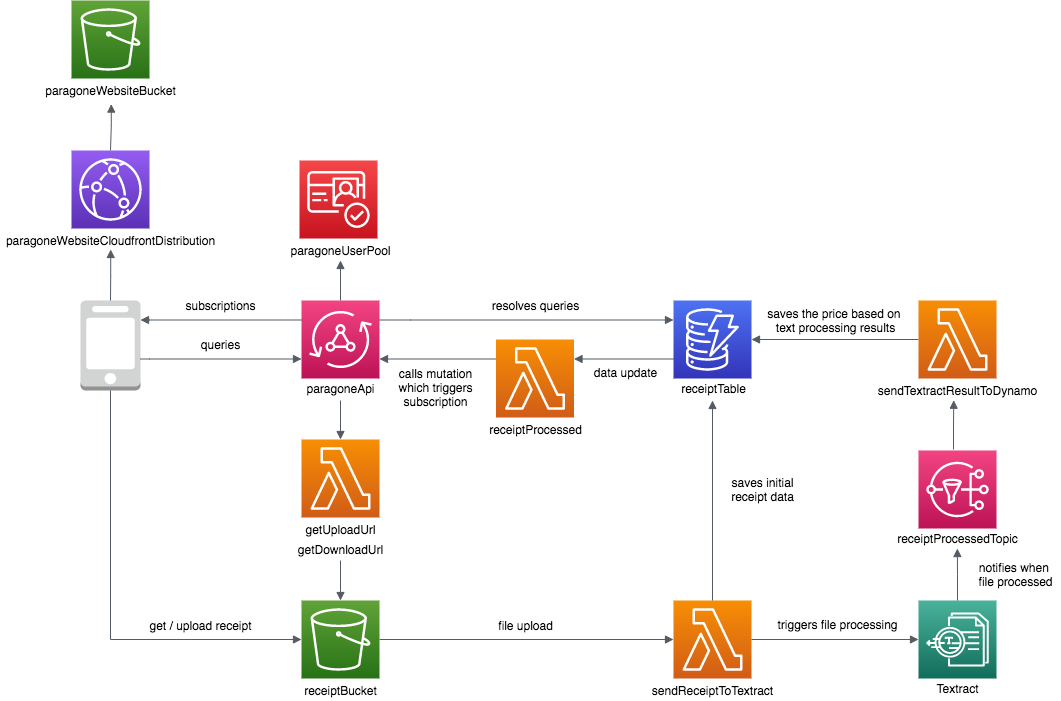
\includegraphics[width=1\textwidth]{assets/04-serverless-for-web-apps/paragoneArchitecture.png}
    \caption{Architecture of receipt processing web application}
    \label{fig:paragone-web-app}
\end{figure}

Key points of the suggested architecture:

\begin{itemize}
    \item \textbf{GraphQL as API} --- Presented example shows the basic backend of the web application built using the serverless technology. AWS AppSync is used to expose the GraphQL API, which is configured to trigger the AWS Lambda or communicate directly with some external services, such as DynamoDB. Moreover, the integration with AWS Cognito introduces the authentication and authorization capabilities to the API. Each of the GraphQL operations, such as queries, mutations and subscriptions can be restricted, to ensure that only logged in users have access to their private data. Once the receipt processing is completed and the data is stored in the database, the user is notified in real-time about the results of the asynchronous operation, based on the established GraphQL subscription. The AWS Lambda, that is polling the DynamoDB for the event stream including inserts and updates for a given table, triggers the GraphQL mutation, which in turn pushes the new data to the client.
    \item \textbf{Secure and direct access to services storing the files} --- The GraphQL API, built on top of the AWS AppSync services, is not designed with intent to handle the operations on the files including downloads and uploads. Instead, the mechanism of presigned URLs is incorporated. It enables the client application to directly communicate with the Amazon S3 in a secure way, to access or store the files with predefined names and within a limited and strictly defined period of time. It alleviates the need of using the AWS Lambda to process and insert the data into the bucket upon the user request, which could be more time consuming operation compared to generating the presigned URL.
    \item \textbf{Asynchronous receipt processing} --- The receipt processing flow is performed in an asynchronous manner, similarly to many other processing flows, utilising the serverless paradigm. Uploading the receipt to Amazon S3 triggers the AWS Lambda, which is responsible for inserting metadata about the image to the database and sending the receipt to Amazon Textract performing the document analysis task. Once the processing is completed, the Amazon SNS receives the event with the job identifier, which further triggers the AWS Lambda subscribing to the particular topic. The serverless function retrieves the data and based on simple heuristics, analyses the results of the text extraction process and stores the information further in DynamoDB.
    \item \textbf{Web application hosting} --- The backend of the application, composed from the combination of configured with each other services mentioned earlier, is effectively hosted in the cloud. Similarly, the client application once built, it can be stored in a publicly available Amazon S3 bucket in the form of the static assets. Amazon CloudFront distribution can be additionally integrated to provide the capabilities of Content Delivery Network, delivering the client application to users in a more convenient way.
\end{itemize}

Along with the simple heuristics retrieving the information based on the text extraction process, the more sophisticated services could be incorporated in the receipt processing flow, for example to categorise the expenses, or provide more detailed spending statistics. Nevertheless, the other services would also operate in the same, asynchronous manner, extending the presented flow and performing the computation in a form of a distributed system composed of several components hosted in the cloud.

\subsubsection{Discussion}

The proposed solution presents the fully fledged web application built using the serverless architecture, including the serverless backend responsible for processing and storing the data along with the client application hosted in the cloud environment.
The presented architecture is also a good illustration of different execution models of the AWS Lambda, covered in more details in section \ref{chapter:lambda-function-execution-model}, including synchronous execution to obtain the presigned URL, creating an asynchronous receipt processing flow as well as polling the stream of updates from the DynamoDB.

The asynchronous processing choreography, described in more details in section \ref{chapter:serverless-processing-function-composition-and-orchestration}, is a common pattern in the serverless architecture and refers to composition of multiple components, responsible for particular chunks of the processing and forming effectively a distributed system.
The AWS Lambda is used to incorporate the business logic of the application, transforming the data when desired and using other services to orchestrate the flow or handle the processing, without waiting idle for the results, but rather being triggered in an event-driven manner.

The use of Amazon Textract brings new development opportunities, allowing to integrate the service in the processing flow with convenient billing per usage and eliminates the need to maintain similar self-hosted service.

AWS AppSync serves as a feature-rich gateway of the application backend, triggering Lambda functions or directly communicating with other services to retrieve the data, but also it allows to update the client in real-time using the subscriptions, which is a beneficial feature for the asynchronous processing.
All of the processing is performed in a secure and compliant way, thanks to the authentication and authorization capabilities introduced by the integration of AWS AppSync with the Amazon Cognito, along with the presigned URL mechanism, enabling it to safely store and retrieve the files from Amazon S3 bucket.

\subsection{Generating interactive slideshow based on LaTeX files} \label{chapter:examples-generating-interactive-slideshow-based-on-latex-files}

\subsubsection{Problem description}

The second example covers an implementation of web application similar to the Pitagoras Korepetytor\footnote{\url{http://pitagoras-korepetytor.pl/}}, which is a service playing a role of the virtual math tutor for high school students.
It provides a large collection of exercises, which can be further adjusted by the users when changing the values of the exercise parameters.
Based on the user input, the service generates an interactive slideshow, which is further previewed by the user in the interactive client application.
The slides present the following steps required to solve the exercise, with the additional audio commentary, explaining the performed mathematical operations.

\subsubsection{Proposed processing flow} \label{chapter:examples-generating-interactive-slideshow-based-on-latex-files-proposed-processing-flow}

When inspecting the processing results of the original solution, the user is given a set of slides along with the audio files, which are later processed by the presentation player on the client side.
Due to the large number of the parameters combinations, that can be specified by the user and their value domains, generating the slides and commentary for all possible input values can occupy a lot of memory and be unprofitable.
Moreover, some of the presentations include advanced math equations, graphics visualising more sophisticated geometry problems or even considering some conditional logic based on parameters, upon which the solution for the exercise is generated.

Taking into consideration the problem and its requirements described above, the LaTeX \cite{latex} typesetting language and its processor is one of the possible solutions for the problem, which is well-known and frequently used in the academia community.
It enables the presentation creator to easily define the mathematical computations, present graphics showing the geometric tasks, which can be also extended based on the defined variables, including even some computations performed by the LaTeX processor or conditional logic.

Taking into account the selected tool, the processing flow for the user request could take the following:

\begin{enumerate}
   \item The initial step, taking place before the processing of the file is started, can be used to validate the user input. The entered values can be compared with the constraints of the exercise along with verifying if the user can preview the particular presentation, based on the application logic of the service.
   \item Once the input is verified and the user is allowed to request the presentation, the exercise variables from the input can be injected into the LaTeX file. 
   Next, the presentation is generated to the PDF file, which is further split into separate slides in the form of SVG files.
   \item Along with the slideshow generation, the initial presentation file can include additional directives with the commentary, which are extracted and supplemented with the variables from the user input. The processed text can be transformed further into the human-like audio commentary using the voice synthesis software.
   \item Additionally, some metadata about the presentation can be retrieved, including the slide durations for the slideshow or the information when to play the audio commentary, which will be sent and used later by the client application.
   \item The steps 2-4 can be performed in parallel. Once they are completed, the result can be afterwards sent to the client to preview the slideshow with the exercise to the user.
\end{enumerate}

The described flow presents a rather extraordinary task incorporated in a web application, which plays a significant role in fulfilling the business logic of the proposed services.
In the traditional architecture, the responsibility of performing the presentation processing could be extracted into a separate service, that triggers one of the worker based on the user requests.
With the limited traffic, the approach with a separate service communicating with a set of workers would be suitable, but when a larger group of users would submit a request to process a request within a short period of time, the scalability of such a system should require to scale the number of available workers accordingly.
The instant scalability of the serverless architecture, with a pay-as-you-go billing model, would be beneficial to meet the variable demand of the presentation processing requests.
Moreover, the high-quality services hosted in the cloud, that are capable of performing the voice synthesis, could be integrated in the solution.
However, processing the LaTeX files using the serverless function is a non-standard type of computation task, which requires the function runtime to be properly enhanced to fulfill the task.

\subsubsection{Designed solution}

The designed solution presented in the diagram, covers the presentation processing workflow along with the communication with the client application, responsible for displaying the slideshow based on the generated data.
The practical research focused on configuring the serverless function, along with the processing optimisations of the described flow, is presented in more detail in section \ref{chapter:latex-processing-optimisation}.

\begin{figure}[H]
   \centering
   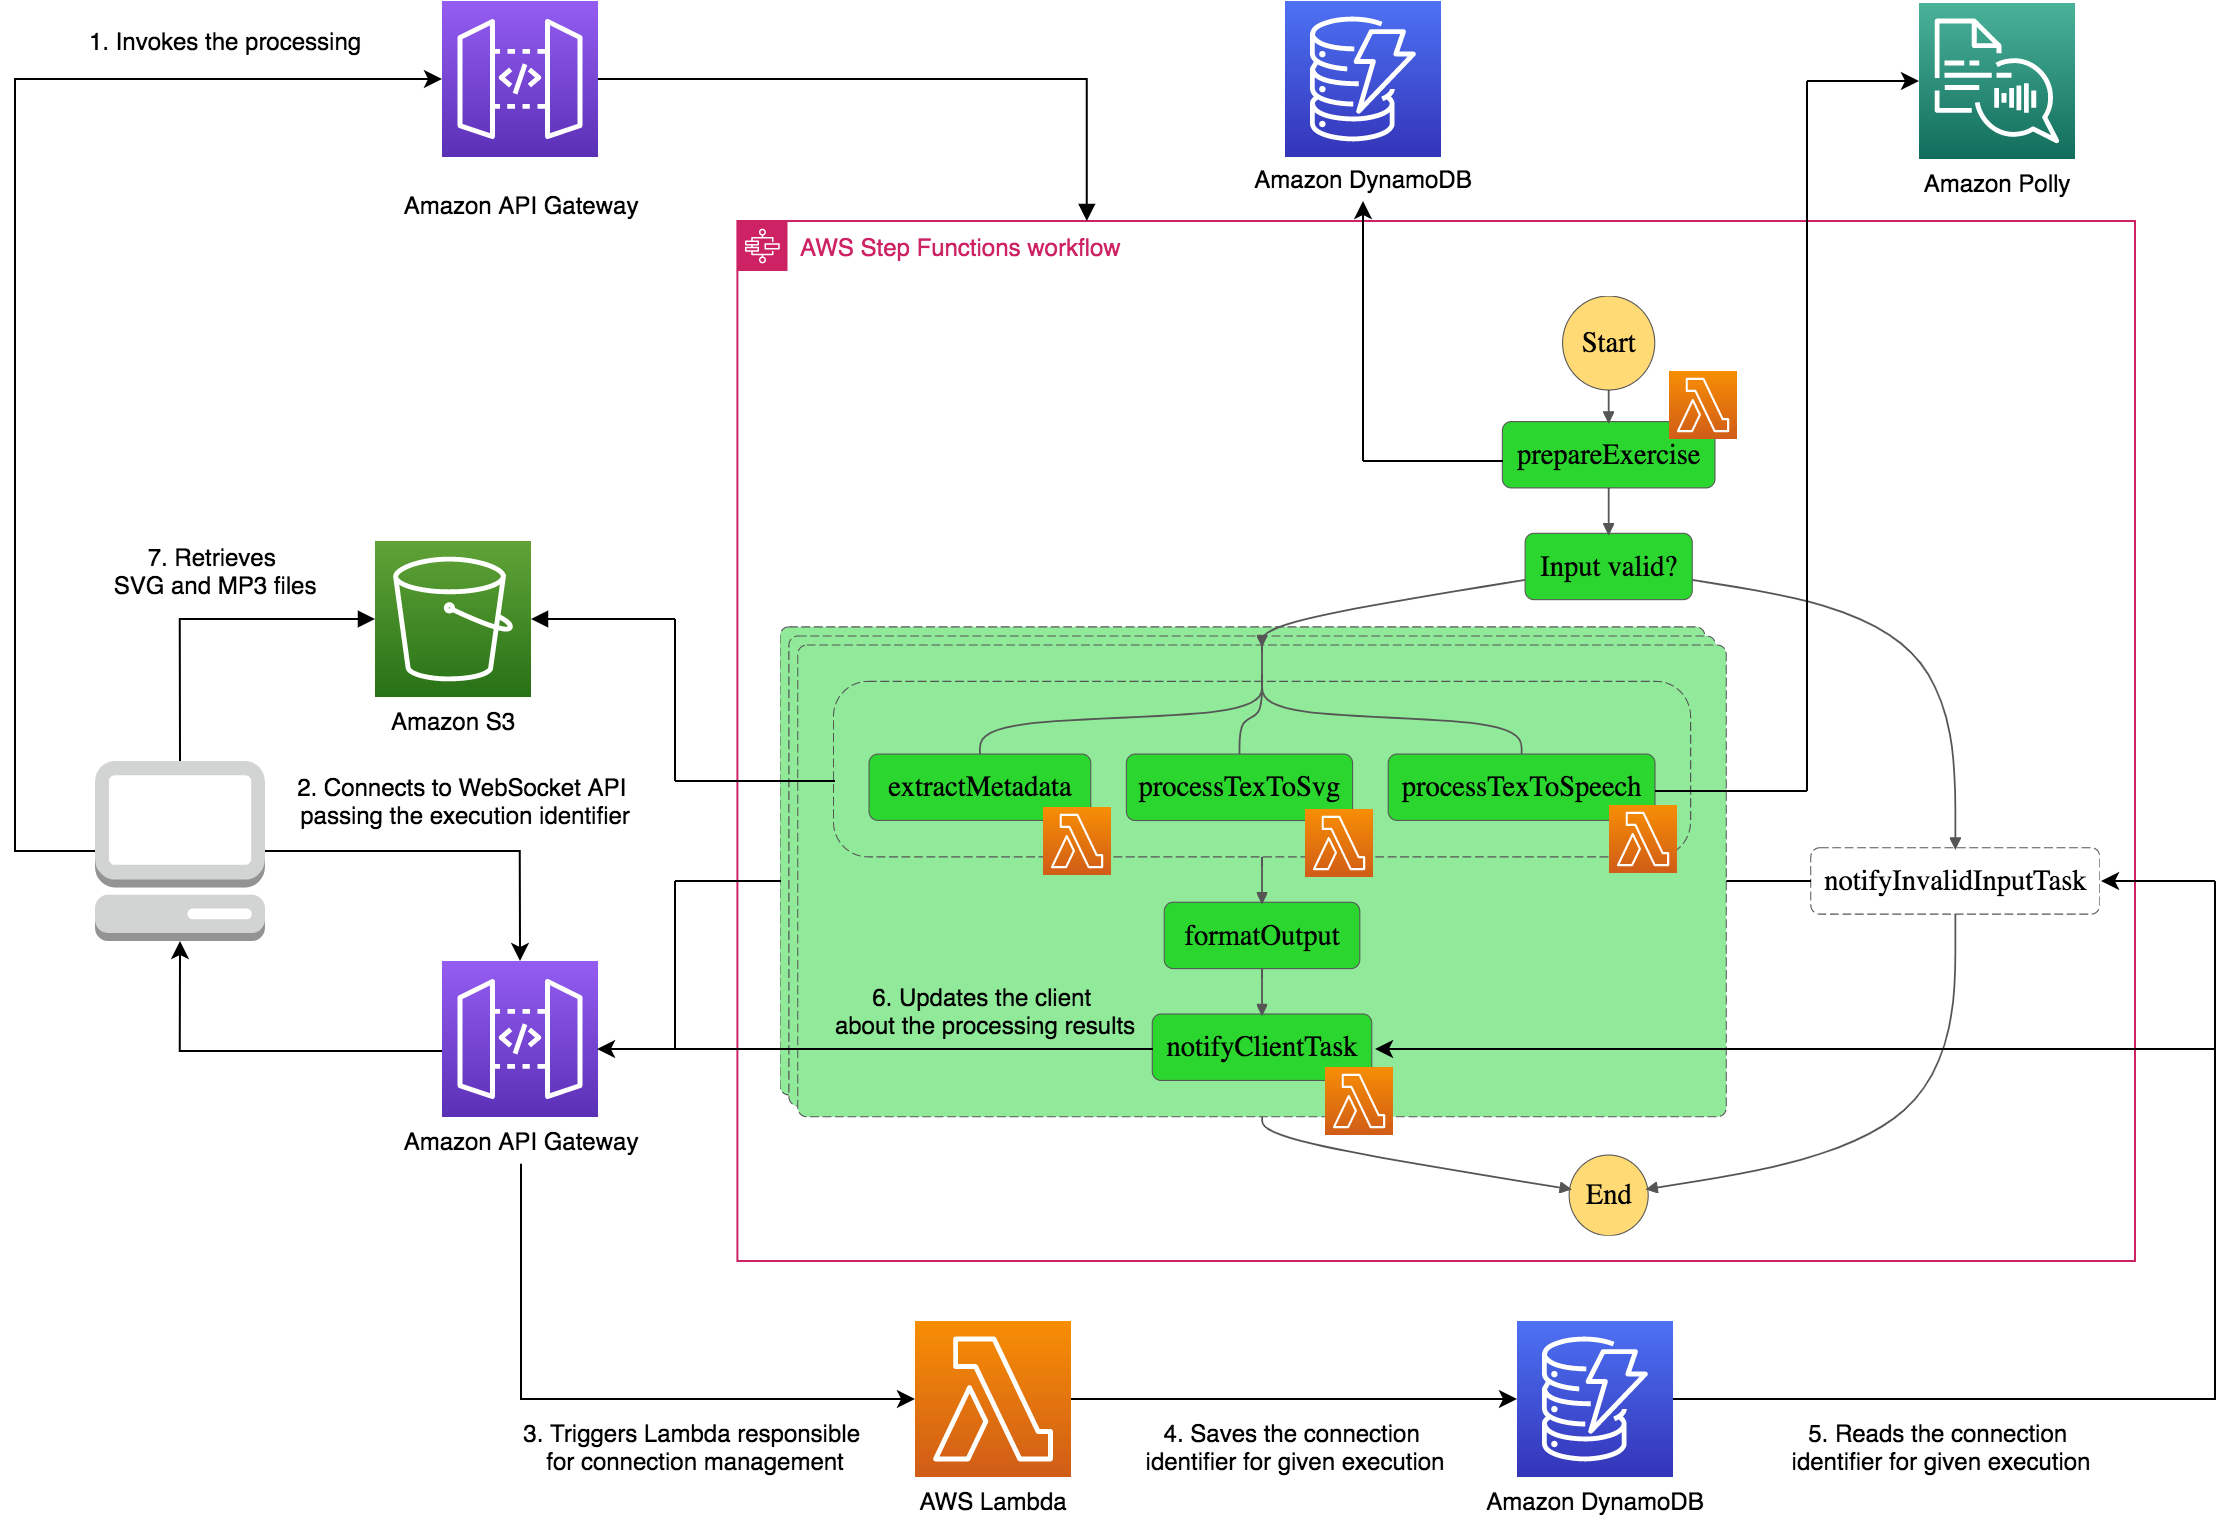
\includegraphics[width=1\textwidth]{assets/04-serverless-for-web-apps/euclidArchitecture.png}
   \caption{Architecture of presentation processing}
   \label{fig:euclid-web-app}
\end{figure}

Key points of the suggested architecture:

\begin{itemize}
   \item \textbf{Function orchestration using the AWS Step Function} --- The presentation processing flow is built on top of several AWS Lambda instances with the AWS Step Function orchestrating the entire process.
   AWS Lambda performs the initial task by retrieving the exercise details, validating the user input against the exercise constraints and defining the tasks for subsequent serverless function invocations, if the provided input satisfies the limitations.
   Based on the output of the first task, the further processing is executed or the user is notified about the invalid request.
   The presentation processing task is further separated into two chunks. 
   The first one generates the slideshow for several initial slides, which is pushed to the client as soon as possible once the processing is completed and starts previewing it to the user. While the second part, including the remaining chunk of the presentation, is delivered to the client later, when the user is busy watching the initial portion of the slideshow.
   For each of the chunks, three AWS Lambda instances are executed concurrently. They are responsible for processing the LaTeX file and extracting the slides in form of the SVG files that are later uploaded to the Amazon S3, generating the voice commentary using the Amazon Polly which are further stored in Amazon S3 as well as extracting some metadata about the generated slideshow.
   Once all three tasks for a given chunk are completed, the output of the functions is formated and another serverless function is invoked to push the results of the processing to the client using the WebSocket API
   \item \textbf{Pushing the update to the client} --- AWS Step Function orchestrates the processing in an asynchronous manner, which makes it necessary to notify the client once the processing is finished.
   Instead of using the polling techniques to periodically check whether the presentation is generated, the push based approach is used.
   Initially, the client application invokes the AWS Step Function and gets its execution ID.
   Next, it connects to the WebSocket API and sends a message with the obtained identifier, invoking the AWS Lambda that stores the execution ID along with the associated connection ID in the DynamoDB.
   When the chunk of the presentation is generated, the serverless function retrieves the data based on the execution ID and sends the message with the processing results to the associated client application.
   Finally, the slides and audio files, stored in the Amazon S3 bucket under predefined path, are retrieved.
\end{itemize}

\subsubsection{Discussion}

The proposed solution describes an interesting and non-standard use case of the serverless processing pipeline, responsible for preparing slideshow with the audio commentary based on the LaTeX files.
The predefined slideshows are requested by the user, making the desired outcome of the processing similar to the MindMup’s exporters service, mentioned in section \ref{chapter:serverless-suitability-mindmup}.

The serverless architecture is an appealing technology for the file processing tasks that are scheduled in an event-driven manner.
The resource allocation based on demand along the autoscaling capabilities with proportional billing and scaling down to zero in absence of requests, makes the serverless technology an applicable and cost efficient solution to use.
However, the processing flow for the described example is more sophisticated and consists of several steps, which requires thoughtful coordination.
It has been re-architectured across several subsequent iterations to leverage the benefits of the serverless architecture and make the slideshow processing more efficient.
The design process along with the performance comparison and cost calculation is presented in more detail in section \ref{chapter:latex-processing-optimisation}.

The proposed solution relies on the orchestration of the processing, that consists of the serverless function invocations, performing various tasks on different steps of the processing.
AWS Step Function enables the processing to preserve state between the function execution along with orchestrating the flow, which can include some branching, tasks executed in parallel, mapping over a list of subtasks and gathering the results of the group of tasks.
The solution brings quite some elasticity when defining the processing schema and provides visualisation of the workflow, giving better insight into the executed processing.
However, the size of accumulated state in the AWS Step Function is strictly limited, which is insufficient to store the results of LaTeX files processing there, and requires the use of Amazon S3 to preserve the processed files from different stages of the computation to make them later available to the user.

Similarly to the previous example, the processing is performed in an asynchronous manner and requires some additional solution to update the client once the results are ready. The proposed solution invokes the AWS Step Function using the REST API and later connects via the WebSocket API to receive notification when the slideshow is available.

Another challenge with the proposed processing flow is related with the LaTeX files processing. The use of Lambda layer, including the additional dependencies, makes it possible to perform such custom tasks and enhance the Lambda runtime with numerous capabilities.

Lastly, the use of the AWS Polly provided another development opportunity, enabling to easily enhance the slideshow with the audio commentary, without the need to host similar service or incorporate some other third party service, running outside of the cloud platform.

\section{Server Tier}

\subsection{Lambda function as a compute resource} \label{chapter:lambda-function-as-a-compute-resource}

The idea of Function as a Service has been already introduced in section \ref{chapter:serverless-faas}.
An example of such FaaS offering is AWS Lambda \cite{AWSLambda}, which is described as a compute service that requires no resource management. It provides the autoscaling capabilities, high-availability built-in and pay-per-use billing model, based on the function execution and the processing time with a granularity of milliseconds. 

The following section analyses in more details the FaaS capabilities, considering the AWS Lambda as one of the implementations of this model, taking into account its limitations, runtime possibilities, execution models and possible optimisations.
Based on the overview of the AWS Lambda functionalities, the intuition of FaaS model capabilities as an execution environment can be established.

\subsubsection{Function limitations}

The AWS Lambda execution is constrained by quotas referring to the compute and storage resource that can be used by the serverless function.
Some of the AWS Lambda restrictions have been already discussed in section \ref{chapter:serverless-processing-limitations-runtime-and-data-restrictions}.
The list below includes additional limitations along with explanation of their impact on the processing of the serverless workloads \cite{AWSLambdaQuotas}.

\begin{itemize}
   \item \textbf{Concurrent executions} --- 1000 executions --- The serverless paradigm ensures about the infinite scalability of the underlying platform, however the default maximum number of functions that can be invoked is limited. It is essential to keep that in mind when developing some serverless solution extensively using the Lambda, that there is some threshold above which the function execution will be throttled. The limit can be increased further by the cloud provider.
   \item \textbf{Function memory allocation} --- from 128 MB to 10240 MB --- The function memory allocation can be configured, which translates into the available CPU and network bandwidth. When the memory of the function is set above the 1769 MB threshold, it provides processors with multiple cores capable of multithreading processing. Therefore, further increase for single threaded computation will increase the memory or bandwidth, which will be suitable accordingly for memory-bound or I/O-bound processing \cite{BecomeAServerlessBlackBelt}.
   \item \textbf{Function timeout} --- 900 seconds (15 minutes) --- The Lambda execution time is strictly limited, which makes it not suitable for processing various long-running tasks
   \item \textbf{Deployment package size} --- 50 MB (zipped) and 250 MB (unzipped, including layers) --- The function deployment package including the function code and its dependencies is constrained as well. The function execution environment can be additionally extended by the Lambda layers including additional code, libraries or dependencies. When the size constraints do not allow to pack all of the required dependencies, the function can be also based on the custom container image limited up to 10 GB. The topic of Lambda layer and container image is discussed further in section \ref{chapter:lambda-custom-runtimes}.
   \item \textbf{Invocation payload} --- 6 MB (synchronous invocation), 256 KB (asynchronous invocation) --- The invocation payload limit is related to the size of an event invoking the Lambda function.
   The synchronous invocation model requires the serverless function to return some value to the service triggering the function, for example the AWS API Gateway invoking the function based on user request, contrary to the asynchronous invocation, triggered for example by uploading some file to Amazon S3.
   The constraint prevents from passing large amounts of data in the event payload and requires the function to communicate with external components to retrieve or save the processing results if required.
   \item \textbf{Temporary directory storage} --- 512 MB --- Each of the invoked function environment is assigned a temporary storage, enabling the function to retrieve some data and perform the required processing in the local file system, which due to the ephemeral nature of the function containers, is further deprovisioned. The results of the processing need to be preserved in some dedicated storage component, depending on the type of the data being stored. Alternatively, under some circumstances, AWS Lambda can utilise the larger storage space when integrated with Amazon Elastic File System, which is a fully managed, shared file system service \cite{AWSLambdaEFS}.
\end{itemize}

Besides the appealing features mentioned at first, such as the Lambda scaling capabilities with proportional billing and the high-availability without the need for managing infrastructure, the further quotas describe how the Lambda runtime is limited.
The constrained execution time shows the limitation of the serverless architecture, along with the limited invocation payload, which requires the function to communicate with external services from Lambda after the invocation. However, thanks to improvements in other areas, the Lambda can be configured to utilise greater amount of memory and multi-core processors, the deployment package can be extended when using the custom container image along with connecting the temporal disc space to the shared file system.
Mentioned enhancement makes it possible to use the AWS Lambda in various, non-standard processing, while leveraging its benefits.

\subsubsection{Function runtime} \label{chapter:lambda-custom-runtimes}

AWS Lambda supports natively several programming languages and their runtime environments including Node.js, Python, Java, C\#, Go and Ruby, with some of them including different versions of the runtime \cite{AWSLambdaRuntimes}. Most frequently the function code and its dependencies are compressed and packed by the deployment tool into a single zip archive and further stored by the cloud provider. When the Lambda function is invoked, the serverless platform allocates the resources to form the function environment, downloads the function code, bootstrap the language runtime with function dependencies and execute the function code. However, when the function has been recently triggered, the execution environment from a previous invocation can be reused, saving time required to prepare the environment and reusing some resources, such as established connections with external services or the temporary files.

Besides the standard function packing option and environment, the AWS Lambda enables to define Lambda layers, enabling to share dependencies irrespectively, between several functions as well as custom container images.
Both of the approaches are described in more details below.

\paragraph{Lambda container image}

With the growth of containers popularity, it become a standard of the web application packing. The AWS Lambda allows to deploy the serverless functions based on custom Docker or OCI images, which enables developers to build serverless functions arbitrary from the supported programming languages and required dependencies \cite{AWSLambdaContainerImage}. Moreover, it allows to process other workloads depending on sizable dependencies, such as machine learning or other data intensive tasks.
Container images are constrained up to 10 GB in size, contrary to the aforementioned limit of the zipped function artifact, which make container images suitable to include custom runtimes, binaries and libraries, that can be used by the serverless function.
AWS provides a set of base images for supported runtimes as well as supported linux base image, however the developers can use any container image if it supports the Lambda Runtime API, which is a simple HTTP-based protocol, responsible for invoking the function and retrieving its results.
The custom container images can be built using familiar tooling and later uploaded to Amazon Elastic Container Registry, from which the image will be retrieved once the function is invoked.

Compared to other services enabling to run container based workloads, the Lambda container image support allows to scale workloads on per request basis and scale to zero with no additional cost if there is no traffic, providing more granular pricing model than other services. Moreover, the Lambda function is integrated with many AWS services, which means that it can be invoked from numerous event sources. 
Nevertheless, the Lambda still needs to satisfy the aforementioned limitations other than artifact size \cite{RunningContainerImagesInAWSLambda}.

\paragraph{Lambda layer}

When taking into consideration the encapsulated nature of the FaaS, several Lambda functions operating in the same part of the application logic can have some common methods, utilities and dependencies, effectively duplicating the same code in every deployed artifact.
Lambda layer is effectively a zip archive including additional code, dependencies and libraries, that can be shared across multiple Lambda functions, reducing the overall size of individual function artifacts.
When including the layer in a function, its content is extracted into function's local file system and can be further accessed by the function code, enabling functions to share common files and mitigating the problem of code duplication.
Moreover, the Lambda layer can include other, operating-system specific libraries and binaries used by the function code as well as custom runtimes, enabling developers to add required dependencies and execute code developed in any programming language in Lambda functions.
The function can include up to 5 layers, with the total size of the function code and layers summing up to 250 MB after decompressing \cite{AWSLambdaLayer}. \\

The serverless function introduces an interesting approach in terms of developing and deploying the function code, which is further managed and executed by the cloud platform. Despite the fact that the set of predefined and supported languages along with provided libraries is quite broad, the AWS Lambda execution runtime is limited.
Its extensions, including the Lambda functions based on the custom container images, enables developers to build the lambda with known container technology, increasing the artifact limit to 10GB, to extend the suitability of the serverless function to other, data-heavy types of workloads.
Moreover, the use of Lambda layers makes it possible to share dependencies easier, across multiple functions as well as introduce external libraries or even custom runtimes, thanks to the Lambda Runtime API.
Both of the described approaches allow developers to adjust the Lambda runtime to perform numerous non-standard tasks.

\subsubsection{Function execution} \label{chapter:lambda-function-execution-model}

The AWS Lambda is executed in an event-driven manner. 
The serverless function can be invoked by each of the defined triggers, configured based on the various event sources, including numerous services from the AWS cloud platform and their operations. 
The generic categorisation of data sources and invocation types for the serverless processing is described in section \ref{section:serverless-function-invocation}. 
AWS Lambda execution model fits into the mentioned classification and distinguish the following types of the function invocation \cite{OptimiseYourServerlessApplications}.
All of the mentioned execution models are present in the example implementation of the receipt processing application, mentioned in section \ref{chapter:examples-receipt-processing}.

\begin{itemize}
    \item \textbf{synchronous (push based)} --- Most frequently refers to the components acting as an API Gateway, invoking the Lambda based on the request and while the function completes the execution, it returns the results to the API Gateway, which passes back the response to the client.
    When Lambda fails during the event processing, the error is returned to the service calling the function.
    In case of the receipt processing application, the AWS AppSync invokes the Lambda functions in a synchronous manner, when user performs query to obtain the presigned URL.
    \item \textbf{asynchronous (event based)} --- Covers all cases in which the service makes a request to the Lambda function, which is consuming an event, but once the execution is completed it has no possibility to return the information to the event source. 
    When the processing fails, the function is retried two more times by default.
    After that the erroneous event can be placed in the Dead Letter Queue or it can be directed to other function, if configured.
    The Lambda function, triggered after the receipt is uploaded to S3 bucket as well as the other one, invoked based on the notification from SNS topic, are the examples of the asynchronous function invocation.
    \item \textbf{stream (poll based)} --- When assigning the stream based services as the data source, Lambda service runs a poller, that is watching for the messages and once they are available, the stream of events forming a batch, can be passed to the function via the asynchronous event.
    If the processing fails for some reason, the whole batch can be retried based on maximum record age or maximum retry attempts, the malformed data can be extracted from the rest of the shard and retried separately from the correctly processed events. When the retry limit is reached, the shard can be sent to the separate SQS queue or SNS topic.
    In the receipt processing application, the Lambda is polling the DynamoDB stream and based on received records, it is responsible for performing the mutation to push the update to the client.
\end{itemize}

\subsubsection{Function optimisations}

The Function as a Service model, heavily utilised in the serverless paradigm as a compute resource, at a first glance seems to be limited with the ability to configure the function and possibilities to optimise its execution, because the cloud provider takes responsibility for provisioning the resources and executing the function.
However, the thorough design of the application architecture along with the proper composition of the function code and its configuration, regarding the event sources and underlying resources, has a significant impact on the performance of the executed function, which transfers directly to the cost of execution.
The possible optimisations and configuration adjustment suggested by various practitioners for optimising the Lambda function execution and improving the configuration are discussed below.

\paragraph{Lambda execution}

In terms of the Lambda function execution, the improvement possibilities can be divided between the cloud provider and the developers implementing the solution. Taking into consideration the function lifecycle, resource allocation along with the downloading function code is handled by the cloud provider, however the size of deployed artifact can have an impact on the cold start duration. Furthermore, the architecture of the function code can have an impact on initialising the function runtime along with required dependencies as well as executing the function code itself.

\begin{itemize}
   \item \textbf{Concise function logic} --- Focusing on developing functions with single purpose and well defined responsibility enables to create leaner functions with fever dependencies, which results with a smaller package once bundled.
   On the contrary to the ''monolithic'' functions, that include some branching logic based on the invocation event to invoke the particular part of the application logic, which takes longer to initialise and can extend the cold start duration \cite{BecomeAServerlessBlackBelt}.
   \item \textbf{Reduce the function dependencies} --- Similarly to the previous point, the amount and size of dependencies transfers to the function initialisation time.
   Depending on the programming language, only selected modules or functions can be imported to incorporate only selected subcomponents of libraries or use techniques like treeshaking to remove unused parts of imported dependencies.
   It allows to obtain smaller function artifacts, with fewer dependencies impacting the function start and execution time \cite{OptimiseYourServerlessApplications}.
   \item \textbf{Use function to transform data, not to transport it} --- Instead of using the Lambda function to transport the data between services, some serverless components from the AWS offering can be integrated to transfer the data directly between each other.
   Similarly, when retrieving the data from external services to the serverless function, it is beneficial to request only the required data instead of performing additional filtering in the function code. It reduces the time, when the function is waiting for an I/O operation, for example when reading the data from DynamoDB or files from S3, that directly reduces the function execution cost \cite{BecomeAServerlessBlackBelt}.
   \item \textbf{Leverage container reuse} --- The conception of the serverless functions assumes that every function execution is stateless and should not rely on existing state from the previous execution.
   However, due to optimisations of the function executions, when the subsequent event triggers the function in a short time after the previous execution is finished, the container environment can be reused along with the initialised runtime and its dependencies.
   The prehandler logic can be used to initialise the connection with external services, such as databases or obtain secrets required in the function handler logic, that can be performed once per runtime initialisation instead of for every function execution.
   Similarly, the function global state can be used as a cache rarely-changing data or lazy-load variables and dependencies, reducing the work and processing time for subsequent invocations \cite{AWSLambdaPerformanceOptimization}.
\end{itemize}

\paragraph{Lambda configuration}

\begin{itemize}
   \item \textbf{Configure function resources intentionally} --- As mentioned before, for each function the amount of memory can be configured, which transforms proportionally to the CPU and network bandwidth configuration.
   Depending on the type of workloads, the function performance can benefit from additional memory for computation, using multiple cores for multithreading processing, when the memory is configured above the 1.8 GB threshold as well as from additional bandwidth for I/O bound processing.
   In terms of the cost the Lambda function is billed per function invocation and execution time, proportionally to the amount of configured memory.
   It is essential to consider, that the function can process the event faster when having more memory, while having similar cost as the function with lower memory configuration that takes longer to finish the processing.
   To better understand the function execution behaviour depending on configuration and take a data-driven approach the AWS Lambda Power Tuning can be used, which is an open-source tool invoking the AWS Step Function executing the function with a set of predefined configurations, measuring the execution time and its cost \cite{BecomeAServerlessBlackBelt}.
   \item \textbf{Select appropriate event sources} --- When configuring the event trigger for the function, it is beneficial to use the configuration options to discard the uninteresting events. For example the message filter for SNS can select only messages with desired payload to invoke the function, while S3 trigger can specify the action performed on the bucket as well as prefix and suffix for the object key, that can be used to trigger the function, based on operation for a file on particular path, filename or extension, if applicable \cite{BecomeAServerlessBlackBelt}.
\end{itemize}

Despite the fact that the cloud provider takes responsibility for managing the underlying infrastructure and execution of function code, the way how the function is structured and configured have a significant impact on its performance.
Applying the knowledge of the Lambda design by keeping the function lean and without unneeded dependencies along with architecturing the application logic in an event-driven manner and leveraging the container reuse to execute the function code more effectively, can greatly improve the performance of the serverless solution.
It is beneficial to keep in mind that the CPU and network bandwidth is allocated proportionally to the configured memory, which can impact how long it takes for the function to execute.
Moreover, proper functions’ trigger configuration enables them to filter out undesired events.

\subsection{Serverless processing model}

Having described the AWS Lambda as an example implementation of the Function as a Service model, it is essential to consider how the serverless function can be incorporated in the application logic.
The event-driven architecture requires some components to trigger the serverless function and as a result receive the response or invoke other components, based on the configuration and code of the function.
Moreover, the stateless and ephemeral nature of the serverless function requires it to communicate with external services to preserve its state.
The serverless architecture relies on various services provided by the cloud platform, which along with the serverless function, make up the application logic \cite{EvaluationOfServerlessApplicationProgrammingModel}.
The simpler application can be composed from the handful of components configured to work together. 
However when the complexity of the system grows, the application architecture composed from numerous independent components, communicating with each in an event-driven manner, creates a more complex distributed system, that can benefit from adhering to microservice architecture patterns, discussed in section \ref{section:web-apps-microservices}.

\subsubsection{Serverless microservices}

The architecture of the web based services built with the serverless architecture can be divided into 2 distinctive categories based on their purpose \cite{AWSReinventBuildingMicroservicesWithAWSLambda}:

\begin{itemize}
   \item \textbf{Public interface} --- Responsible for exposing rich and flexible APIs, most frequently using HTTP protocol to communicate directly with the web based clients. It is using the API Gateway component or other services responsible for load balancing the requests, executing the serverless function, most frequently in a synchronous manner, and returning its results to the client.
   \item \textbf{Internal services} --- Supporting the public interfaces by providing various application capabilities. Moreover, the underlying architecture can utilise the asynchronous processing, passing events with more opinionated structure, leveraging other serverless components with simpler interfaces to decouple the internal services and exchange messages using intermediaries.
\end{itemize}

\paragraph{Public interface} \label{chapter:public-interfaces}

The simpler web services can effectively be based on a handful of components to provide the basic functionalities. Services such as API Gateway can trigger the Lambda function, which in turn communicates with the downstream service, responsible for storing the data, performing certain operations and returning back with the response, as presented in the Figure \ref{fig:simple-web-service-diagram}.

\begin{figure}[H]
   \centering
   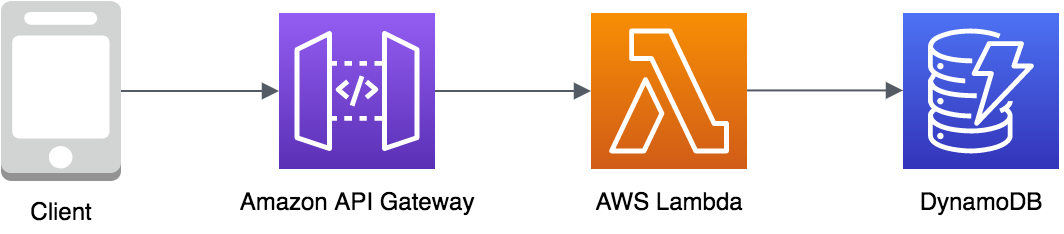
\includegraphics[width=0.7\textwidth]{assets/04-serverless-for-web-apps/simpleWebService.png}
   \caption{Architecture diagram of simple web service using API Gateway, Lambda and DynamoDB}
   \label{fig:simple-web-service-diagram}
\end{figure}

There are several components provided by the AWS, which can serve a role of the public, client-faced interface of the web application, and integrate with Lambda and other hosted services directly \cite{AWSReinventBuildingMicroservicesWithAWSLambda}. The services and their capabilities are listed below:

\begin{itemize}
   \item Amazon API Gateway ---
   Fully managed service enabling developers to define APIs, serving as a front door to the application, integrating with various services hosted in the cloud platform.
   The service distinguished several types of the API including REST API (providing variety of additional features such as API caching, additional transformation and validation of requests, tighter integration with other services), WebSocket API as well as HTTP API (simpler and cheaper compared to REST APIs, providing only basic additional features).
   Moreover, The API Gateway can also provide additional capabilities such as caching, request throttling, different usage tiers for specified clients, security control as well as integration with other services incorporating authentication and authorisation capabilities.
   \item Application Load Balancer ---
   Belongs to the family of the load balancer offerings and it is supporting the HTTP traffic, regardless of the transmission protocol used on top of it.
   The requests are forwarded, based on the URL and HTTP method, to the Lambda or other services according to the configuration.
   Using Application Load Balancer can be cost effective when the service is experiencing high throughput and the requests can be passed directly to the associated services.
   \item AWS AppSync ---
   Managed service, providing the capabilities to define GraphQL APIs, which can map the particular requests to various services, pulling the data from various data sources for a single request.
   Moreover, it can incorporate caching on the server and client side to improve performance, leverage GraphQL subscriptions for real-time communication as well as integrate with other services to provide authentication and authorization capabilities.
\end{itemize}

All of the mentioned components provide the capabilities of exposing an API, which serves as an entrypoint for the application logic.
Besides accepting the user requests and redirecting them to specified components, some of the services enable additional capabilities such as caching, traffic management, request filtering and transformation, authentication and authorization as well as throttling the requests to protect the backend services.
The definition of an API can be generated along with the documentation, when using tools like Swagger \cite{ImplementingMicroservicesOnAWS}.
The additional capabilities of mentioned components are covered in more detail in section \ref{chapter:serverless-client-communication-patterns-for-serverless-architecture}.

Another frequently considered topic, when using the services like API Gateway, is where to perform the routing of the request.
The Lambda code can effectively use one of the frameworks to provide some additional routing inside the handler logic, granting better portability.
However, such approach introduces several challenges, which include applying the security constructs and performance configuration to the whole monolithic function as well as making the proper logging, monitoring and debugging more difficult to implement \cite{AWSReinventBuildingMicroservicesWithAWSLambda}.

\paragraph{Internal services} \label{chapter:interal-services}

The synchronous model of the public interface can work effectively with simpler services, communicating with other serverless components and returning the response back to the client.
However, when the communication is more complex and it includes several services, passing messages to each other, there are several places when the errors can occur, making some of the components waiting for response \cite{AWSReinventBuildingMicroservicesWithAWSLambda}.
When the application is experiencing heavier load, the services communicating in a synchronous manner and leveraging the serverless technologies can observe timeouts and throttling as well as increased cost related with the Lambda functions executing longer and waiting for responses from the polled services.
The API Gateway is configured with maximum integration timeout for synchronous function invocation equal to 29 seconds, after which it returns an error to the client.
Moreover, the function execution time limited to 15 minutes along with its rapid scalability, can be more challenging when communicating with some external or legacy services, that are not capable to scale accordingly, which requires to manage the number of active connections \cite{ServerlessAtScaleDesignPatternsAndOptimizations}.

One of the solutions for the mentioned problem, is to rethink how the communication between components works and redesign it to incorporate asynchronous workflows.
It introduces a similar approach as with microservice architecture, making the components decoupled by using some intermediaries like message brokers to exchange and preserve the events occuring in the system in a reliable way.
The API Gateway request can trigger the AWS Lambda, which in turn communicates with some other service, starting the asynchronous processing and returning the invocation status to the API Gateway, responding to the user.
The processing flow can further get through several services, responsible for processing the application logic and preserving the state accordingly, using some of the serverless platform components to exchange the messages reliably, without tight coupling between services and serverless functions.
The communication with external or legacy systems can be appropriately buffered and throttled to prevent from losing events and affecting their performance \cite{ServerlessAtScaleDesignPatternsAndOptimizations}.
Some of the more complex workflows may benefit from the orchestration of the processing using services such as AWS Step Function, which is described in more detail in section \ref{chapter:serverless-processing-function-composition-and-orchestration}. \\

Components provided by AWS, serving the role of queues, message brokers and message buses as well as services streaming the events, enables the developers to decouple the services and redesign the flow to embrace reliable asynchronous processing, are described below:

\begin{itemize}
   \item Simple Notification Service (SNS) ---
   Managed publish-subscribe messaging service with an ability to reliably exchange messages with low latency, pushing and delivering the messages to other components subscribing to a predefined topic.
   SNS provides high throughput with autoscaling capabilities, allowing to fanout the messages, storing them durably across multiple Availability Zones, but providing no additional persistence beyond retry logic, tracking failures when lambda is not available.
   The events can be filtered based on the message attributes, pushing the event only to selected subscribers.   
   The messages can trigger Lambda function or be published to HTTP endpoints, services such as Amazon SQS or Amazon Kinesis Data Firehose, email, SMS or mobile push \cite{ChoosingEventsQueuesTopicsAndStreamsInYourServerlessApplication}.
   In case of serverless functions, each of the published messages translates to single Lambda execution, however its concurrency can be limited as well as additional configuration can be applied to expose parameters allowing to ensure the FIFO ordering and deduplication of events, however by default the SNS does not provide such guarantees.
   SNS is designed for unidirectional and fanout communication, targeted primarily to Lambda function or HTTP based endpoints.

   \item Simple Queue Service (SQS) ---
   Managed message queue service, storing and exchanging the messages between various software components, reliably preserving them without requiring the service to be available.
   SQS is scaling automatically with configurable batch size, storing the messages durably across multiple Availability Zones with an ability to persist them from 60 seconds to 14 days.
   The batch of messages is polled by one of the consumers, becoming unavailable for others. Once the messages from the whole batch are successfully processed, they are removed from the queue, otherwise they become available to be picked up again after the visibility timeout expires.
   It enables the queue to buffer and rate limit the incoming events, securing the connected downstream services from bursty traffic.
   With standard configuration the SQS provides best effort message ordering, with at least once delivery, guaranteeing high throughput with lower cost. However the service can be configured to expose additional information, enabling downstream services to order and deduplicate the incoming events.
   SQS finds applicability when the incoming traffic needs to be stored in a reliable way and buffered to be further consumed by downstream services \cite{AWSReinventScalableServerlessEventDrivenArchitecturesWithSNSSQSLambda}.

   \item Amazon Kinesis Streams ---
   Highly scalable, managed services responsible for collecting and processing real-time streams of data coming from various sources, including data and video streams, enabling the application to preserve the data and analyse it.
   The data stream is split into multiple shards, based on defined buffer capacity and time interval, passing the payload to the Lambda functions which are polling the stream, providing the data to multiple services.
   The data throughput can be limited by batch size or Lambda concurrency, durably storing the messages across multiple Availability Zones and persisting them up to 7 days if configured.
   The processing failures can be handled by retrying the events in order from a shard based on a checkpoints.
   The shard is processed until successful completion or it can be split to extract the erroneous records, handled separately \cite{ChoosingEventsQueuesTopicsAndStreamsInYourServerlessApplication}.
   Amazon Kinesis Streams are frequently used for real-time processing with massive throughput of data, tracking the order of records and gathering the data stream from multiple consumers, such as logs, sensor data or financial transactions.
  
   \item Amazon EventBridge ---
   Serving a role of serverless event bus, observing the events from various data sources, including AWS services, developed applications and integrated SaaS providers. The events can be further filtered out based on defined rules and routed to the downstream consumers, which receive the events reliably, while their producers can remain decoupled.
   EventBridge enables the application components to exchange messages together by ingesting and routing the data across underlying infrastructure, applications as well as external services.
   The messages are stored durably across multiple Availability Zones, however the service does not provide additional events persistence.
   EventBridge finds applicability when the application requires to connect a lot of different services, including external integrations, while providing granular target rules to filter out the traffic \cite{ChoosingEventsQueuesTopicsAndStreamsInYourServerlessApplication}.
\end{itemize}

The mentioned services are not mutually exclusive and can be combined together to utilise their features and provide desired capabilities to the web application architecture as well as enable effective communication by invoking serverless functions in an event-driven manner.
Some of the patterns including described components and leveraging their capabilities are covered below:

\begin{itemize}
   \item Throttling and buffering --- The autoscaling capabilities of the Lambda function can be a problem for the downstream services, including for example the hosted relational databases, which may not be able to scale accordingly or exhaust the available connections pool.
   SQS and Kinesis Data Streams can be used to persist and batch the incoming events.
   Both of the mentioned approaches can limit the concurrency of incoming traffic, serving a role of buffer, aggregating the incoming requests and executing the function with a single batch or shard, leading to lower cost per function invocation.
   DLQ can be configured to store failed records. Alternatively, Lambda Destination can be leveraged to execute another Lambda function with an event including context of the failure \cite{ServerlessArchitecturalPatternsAndBestPractices}.
  
   \begin{figure}[H]
       \centering
       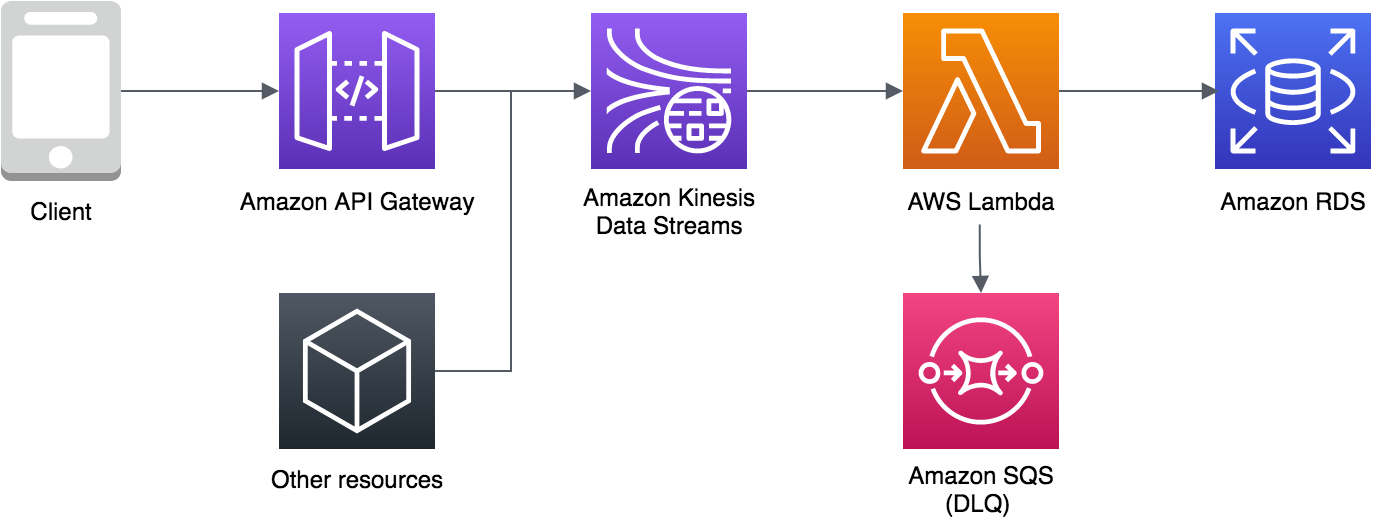
\includegraphics[width=0.8\textwidth]{assets/04-serverless-for-web-apps/buffer.png}
       \caption{Architecture diagram of service using Kinesis Data Streams to throttle and buffer the incoming data}
       \label{fig:throttling-and-buffering-diagram}
   \end{figure}

   \item Fan-Out --- When the payload does not require additional processing, the event can be sent directly to SNS, which pushes the message to subscribers based on the configured filtering. SQS can be configured to subscribe for the events published by SNS, batch the incoming data and share it further with connected Lambda functions or other services.
   Alternatively, for the traffic characterized with high, consistent throughput and large payloads, Kinesis Data Stream can be a more cost efficient solution \cite{ServerlessArchitecturalPatternsAndBestPractices}.

   \begin{figure}[H]
       \centering
       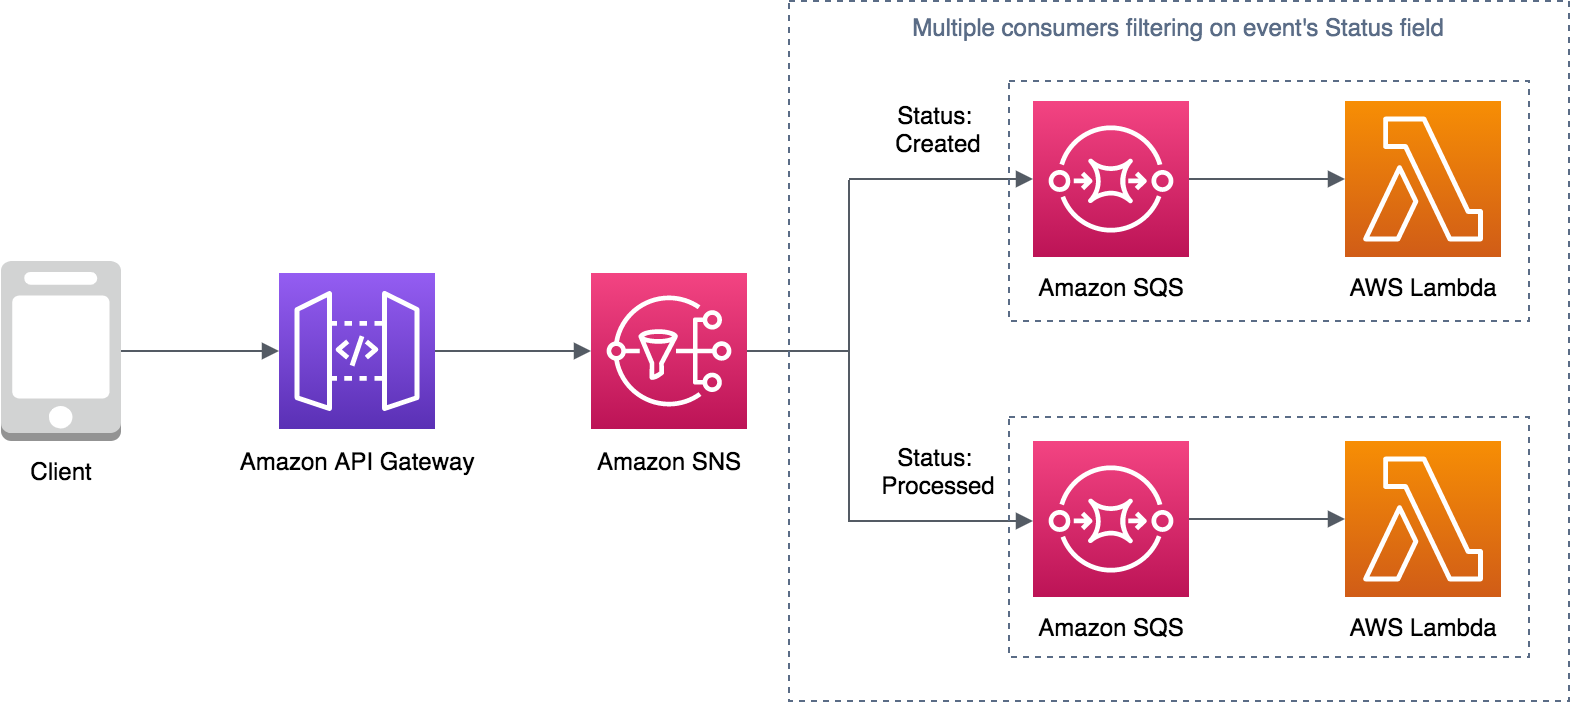
\includegraphics[width=0.8\textwidth]{assets/04-serverless-for-web-apps/fanout.png}
       \caption{Architecture diagram of the Fanout pattern including SNS and SQS to reliably send out events}
       \label{fig:fanout-diagram}
   \end{figure}
   \item Streaming --- The data coming from various data sources can be effectively processed and stored for further analytical purposes. SNS can be used to discard unwanted events, filter the incoming events based on the different business areas and pass the data to Kinesis Firehose to preserve the data, for example in S3 \cite{ServerlessArchitecturalPatternsAndBestPractices}.
   % https://aws.amazon.com/blogs/compute/introducing-message-archiving-and-analytics-for-amazon-sns/
  
   \begin{figure}[H]
       \centering
       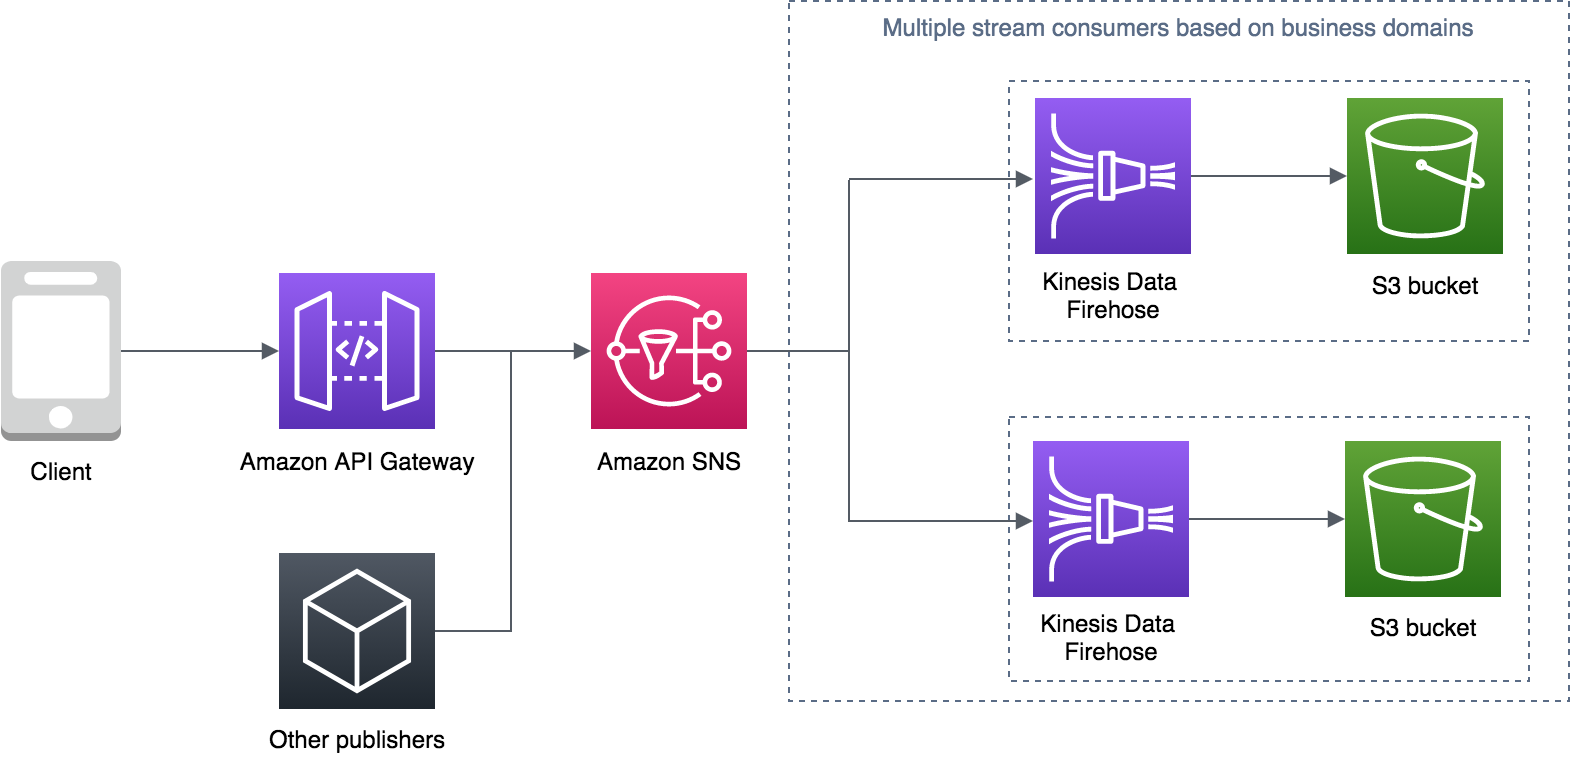
\includegraphics[width=0.8\textwidth]{assets/04-serverless-for-web-apps/streamer.png}
       \caption{Architecture diagram of SNS and Kinesis Firehose preserving the incoming stream of events in S3 bucket}
       \label{fig:streaming-diagram}
   \end{figure}
\end{itemize}

\paragraph{Serverless microservices}

Besides the components serving the role of the entrypoint to the web application and the internal services, responsible for messaging between application components, there are also other components taking an integral role in the applications built in the serverless paradigm as well as shaping its architecture.
The databases capable of preserving the data and reacting to its changes by streaming the updates to polling services are described in more detail in section \ref{chapter:serverless-datastores}.
Moreover, numerous services hosted in the cloud provide various capabilities, including for example image processing, video transcoding or natural language processing, which can be easily integrated in the developed web applications.

The first of the described examples, presented in section \ref{chapter:examples-receipt-processing}, shows how the S3 and DynamoDB are incorporated in the application logic to preserve the images and results of the processing as well as notifying other components about data changes.
Textract is incorporated in the asynchronous processing flow to analyze the uploaded receipts and later publish the results to SNS, fitting into the asynchronous event-driven processing.

When the serverless solution evolves and grows in complexity, it is beneficial to split the application logic into separate domains with well-defined boundaries based on the business capabilities.
It resembles the microservice architectural pattern, described in section \ref{section:web-apps-microservices}, which refers to a set of small services running on its own, communicating via message passing and focused around specific business capabilities.

The serverless microservices are going a step further, splitting the business logic across several serverless functions.
Each of them is responsible for handling and responding to specific events, with the application logic isolated for particular workflow along with granular configuration in terms of access to external services, underlying resource configuration as well as individual selection of technology and libraries to serve its role effectively.
However, most frequently the serverless functions working within the same service boundary and using the same data sources, define some shared library of methods, extracting the business logic from the function handler, responsible for executing the function, and abstracting away the communication with underlying resources.
Each of the serverless functions include the required methods from the shared library to perform the processing, which are packed along the function handler in the deployment process, reducing the functionalities duplication.

Each of the microservices can operate on its own domain and communicate with others via message passing.
To achieve that, each service should expose an interface to make other services retrieve information or perform defined actions.
Moreover, if the operation in one of the services should affect others, it can publish a message to some intermediaries, notifying other components subscribing for changes to react for them appropriately.
Some serverless functions can be designed to serve as a router, providing the API for other services to communicate with as well as receiver, subscribing for the messages from other components, such as SNS or EventBridge, to trigger the further processing.
It enables the serverless microservices to preserve the loose coupling between different microservices, making the services know as little as possible about the implementation of others, communicate via well-defined interfaces, as well as maintain high cohesion within the same service to effectively manage the business domains \cite{AnIntroductionToServerlessMicroservices}. \\

The described serverless microservice architecture enables developers to leverage the benefits mentioned for the microservice architecture itself.
By decomposing and separating the systems into independent components, it is easier to maintain the system over time, introduce required changes and evolve the application. Different teams can manage and develop different parts of the application, focusing on desired capabilities of the services, deciding on programming languages, libraries, data stores to meet the service requirements as well as deploying, configuring and scaling the services independently.

Moreover, various processes and design principles from the microservices architectural pattern can be also applied to the application built using the serverless paradigm.
The decentralized data management allows services to preserve their state independently, but propagating the more demanding operations in an asynchronous way, requires more sophisticated coordination mechanisms to reliably process the transactions, handle failures and retries, utilising the eventual consistency.
Decoupling components make it easier to develop services independently, however such a distributed system requires some communication mechanisms between its elements.
Exchanging messages via intermediaries, service contracts as well as designing for failure, are necessary to make the serverless web application work properly.
Lastly, the automation that is set up properly, providing continuous integration and deployment, is necessary to make the development process manageable.
Automated end to end testing on the deployed environment is essential to give enough confidence that the system works properly as well as proper logging, monitoring and observability are required to track the system capabilities and trigger alarms in case of inconsistencies. \\

Summarising, according to Jeremy Daly in his article describing the various serverless patterns \cite{ServerlessMicroservicePatternsForAWS}, the serverless microservices benefits from adhering the following principles:

\begin{itemize}
   \item \textbf{Ownership of the service private data} --- Each of the serverless microservices should own its data. If another service requires the same data, it should be replicated or it is an indication that the services should be combined together or the application architecture should be rethought.
   \item \textbf{Independent deployments} --- The microservices should be independent and self contained. The dependencies and communication should be based on well defined interfaces and handled by intermediaries to ensure the services are loosely coupled. Maintaining this capability allows developers to independently develop, evolve and deploy the services.
   \item \textbf{Utilising eventual consistency} --- The data replication and denormalisation are commonly used in the microservice architecture and the same solution can be applied in the serverless architecture.
   \item \textbf{Using asynchronous workloads} ---
   With the Lambda function billed for the processing time, it is cost effective to consider the asynchronous processing, instead of making the function wait idle or making the processing to reach the timeout.
   Frequently, the processing can be redesigned to hand off the task, which is reliably processed in the background in an asynchronous manner.
   For use cases that require more complicated coordination, the services provided by the cloud platform can be used, keeping the serverless function small, having a single and well-defined purpose.
   \item \textbf{Keeping the service small, but valuable} ---
   With the granularity and elasticity of the serverless architectures, it is applicable to create even some smaller microservices including only a few functions, if they serve their role well and deliver business value.
   Based on the changing requirements and evolution of the application these can be easily relocated to suit the need.
\end{itemize}

\subsubsection{Function choreography and orchestration} \label{chapter:serverless-processing-function-composition-and-orchestration}

The architecture of the serverless function is suitable for the event-driven workflows, in which communication between subsequent components is managed by services such as SNS, SQS and EventBridge, is asynchronous and loosely coupled.
However, some of the operations require a more fine-grained orchestration approach, with capability to preserve the state between subsequent invocations and give more insight into the business context of performed operations.

AWS Step Function is an example of a service providing capabilities of orchestrating the workflow and managing its state.
Step Function enables to define a state machine, responsible for resembling the business workflow as well as triggering individual components and Lambda functions to avoid additional coordination in the code of the services.
It provides necessary abstraction to define sequential and parallel tasks, branching logic, mapping over a set of tasks as well as handling errors and retry logic.
Moreover, the service allows developers to reason about the state of the executed workflow by visualising the components of the orchestrated flow along their state at individual stages of processing \cite{ImplementingMicroservicesOnAWS}.

In the sections below, the choreography and orchestration of the workflows are described in more detail, as two frequently distinguished modes of the interaction in the serverless microservices architecture.

\paragraph{Choreography}

The choreography refers to an asynchronous, event-driven processing, in which services work independently, using intermediaries in form of message brokers and queues to pass the events to other components invoked further, forming the chain of component invocation performing the business logic.
The interaction model is suitable for simpler operations, when services are not closely related and most frequently belong to separate business domains.
The choreography approach is used in the receipt processing flow, presented in section \ref{chapter:examples-receipt-processing}.

The benefits of such an approach include loose coupling of the services, which can be changed and scaled independently. There is no single point of failure in the system, in which the events can bring additional business value, when processed in the business intelligence reports.
On the other hand, monitoring and reporting in the choreography approach is more challenging, along handling errors, retry mechanisms and timeouts. The business flow is not captured explicitly, instead it is spread across several loosely coupled services \cite{ChoreographyVsOrchestrationInServerlessMicroservices}.

An example architecture diagram of the food ordering workflow, modeled in the choreography approach based on the article written by Yan Cui \cite{ChoreographyVsOrchestrationInTheLandOfServerless}, is presented in Figure \ref{fig:choreography-diagram}.

\begin{figure}[H]
   \centering
   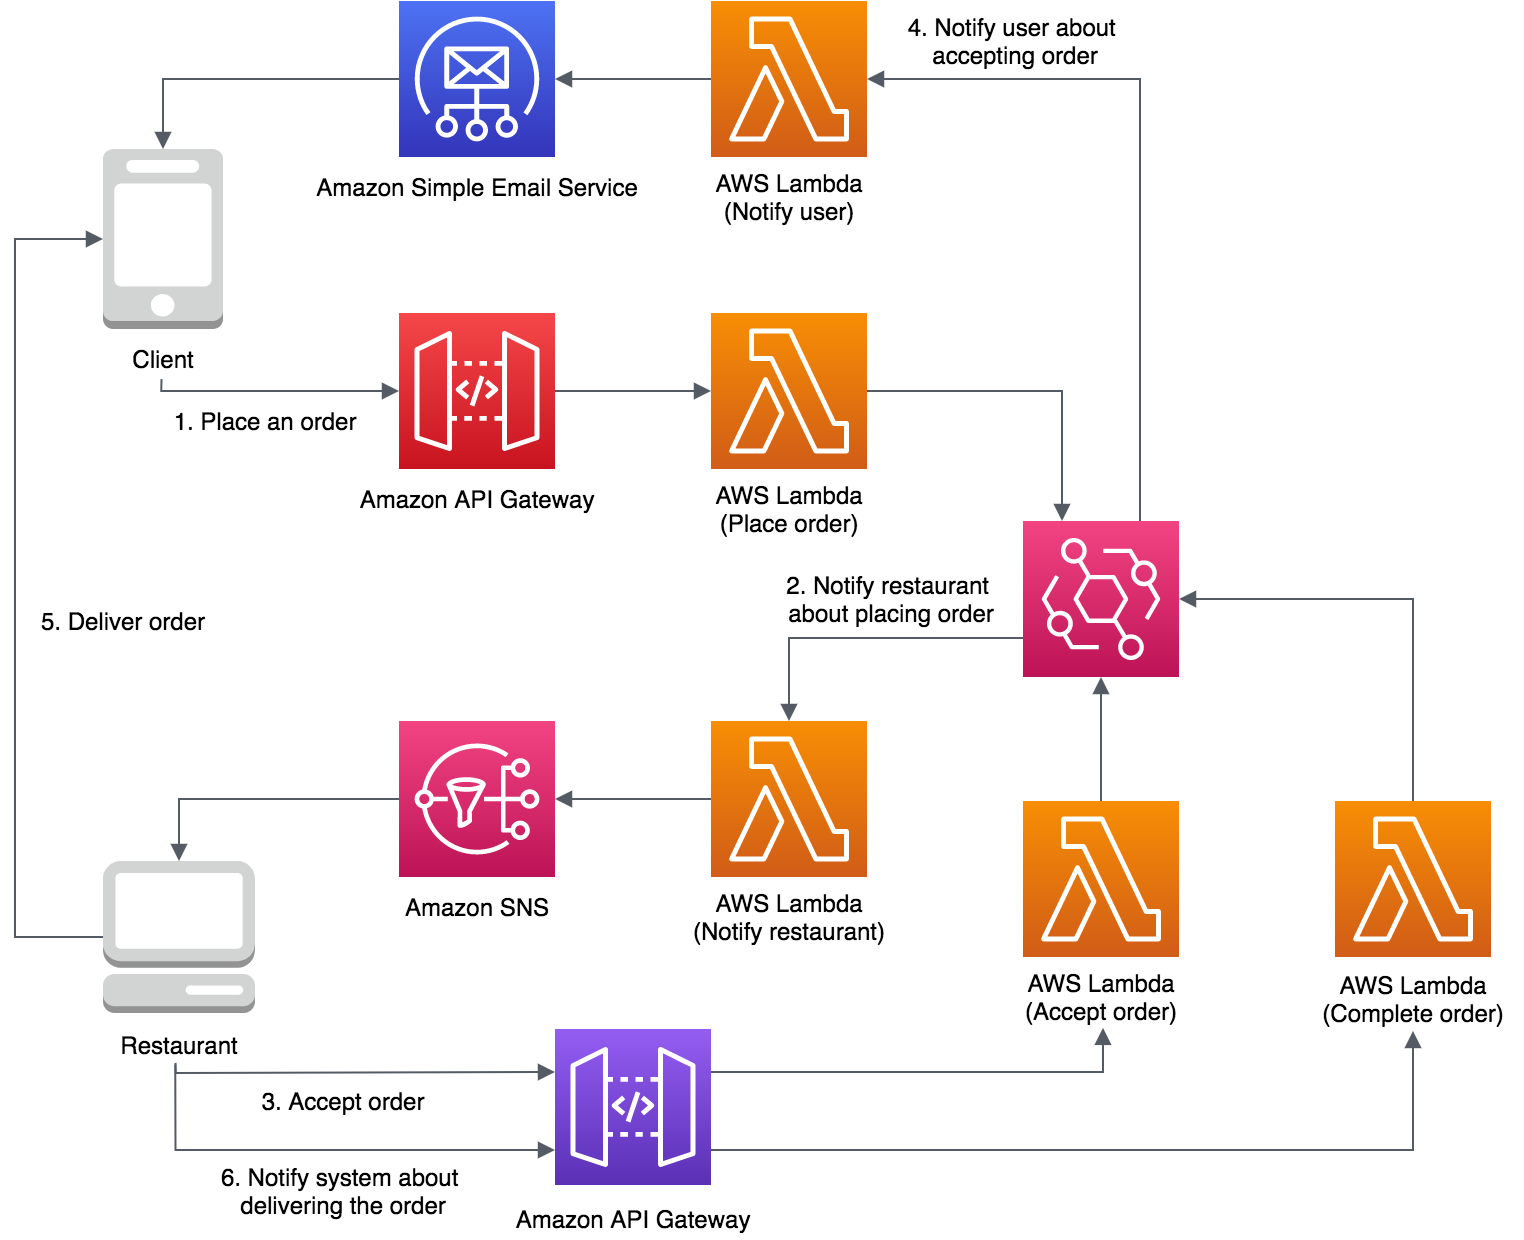
\includegraphics[width=0.8\textwidth]{assets/04-serverless-for-web-apps/choreography.png}
   \caption{The food delivery workflow modeled using the choreography approach}
   \label{fig:choreography-diagram}
\end{figure}

\paragraph{Orchestration}

Instead of configuring services to call each other, the orchestration approach refers to using some dedicated orchestrator component, serving a central role in the processing, coordinating the execution of components, handling interactions between them and maintaining state of the processing, along with handling retries and failures.
Workflow orchestration finds applicability in more complex operations, that require sophisticated flow control, aggregation of resources from different sources and handling the cooperation between microservices in a reliable way.
The orchestration approach is used in the second example implementation, considering the orchestration of generating interactive slideshows, covered in section \ref{chapter:examples-generating-interactive-slideshow-based-on-latex-files}.

The orchestration approach enables the developers to capture the business flow of the process, apply error handling and retry policies, along with removing the need to provide additional logic to handle it in the services.
The workflow logic is contained in one place, providing additional monitoring and visualising capabilities to reason about the status of the processing.
The downside of orchestration include additional cost related with work of the orchestrator, which is a single point of failure in the processing and makes the incorporated components more tightly coupled \cite{ChoreographyVsOrchestrationInServerlessMicroservices}.

Aforementioned example of the food ordering workflow, modeleted in the orchestration approach, is presented in Figure \ref{fig:orchestration-diagram}.

\begin{figure}[H]
   \centering
   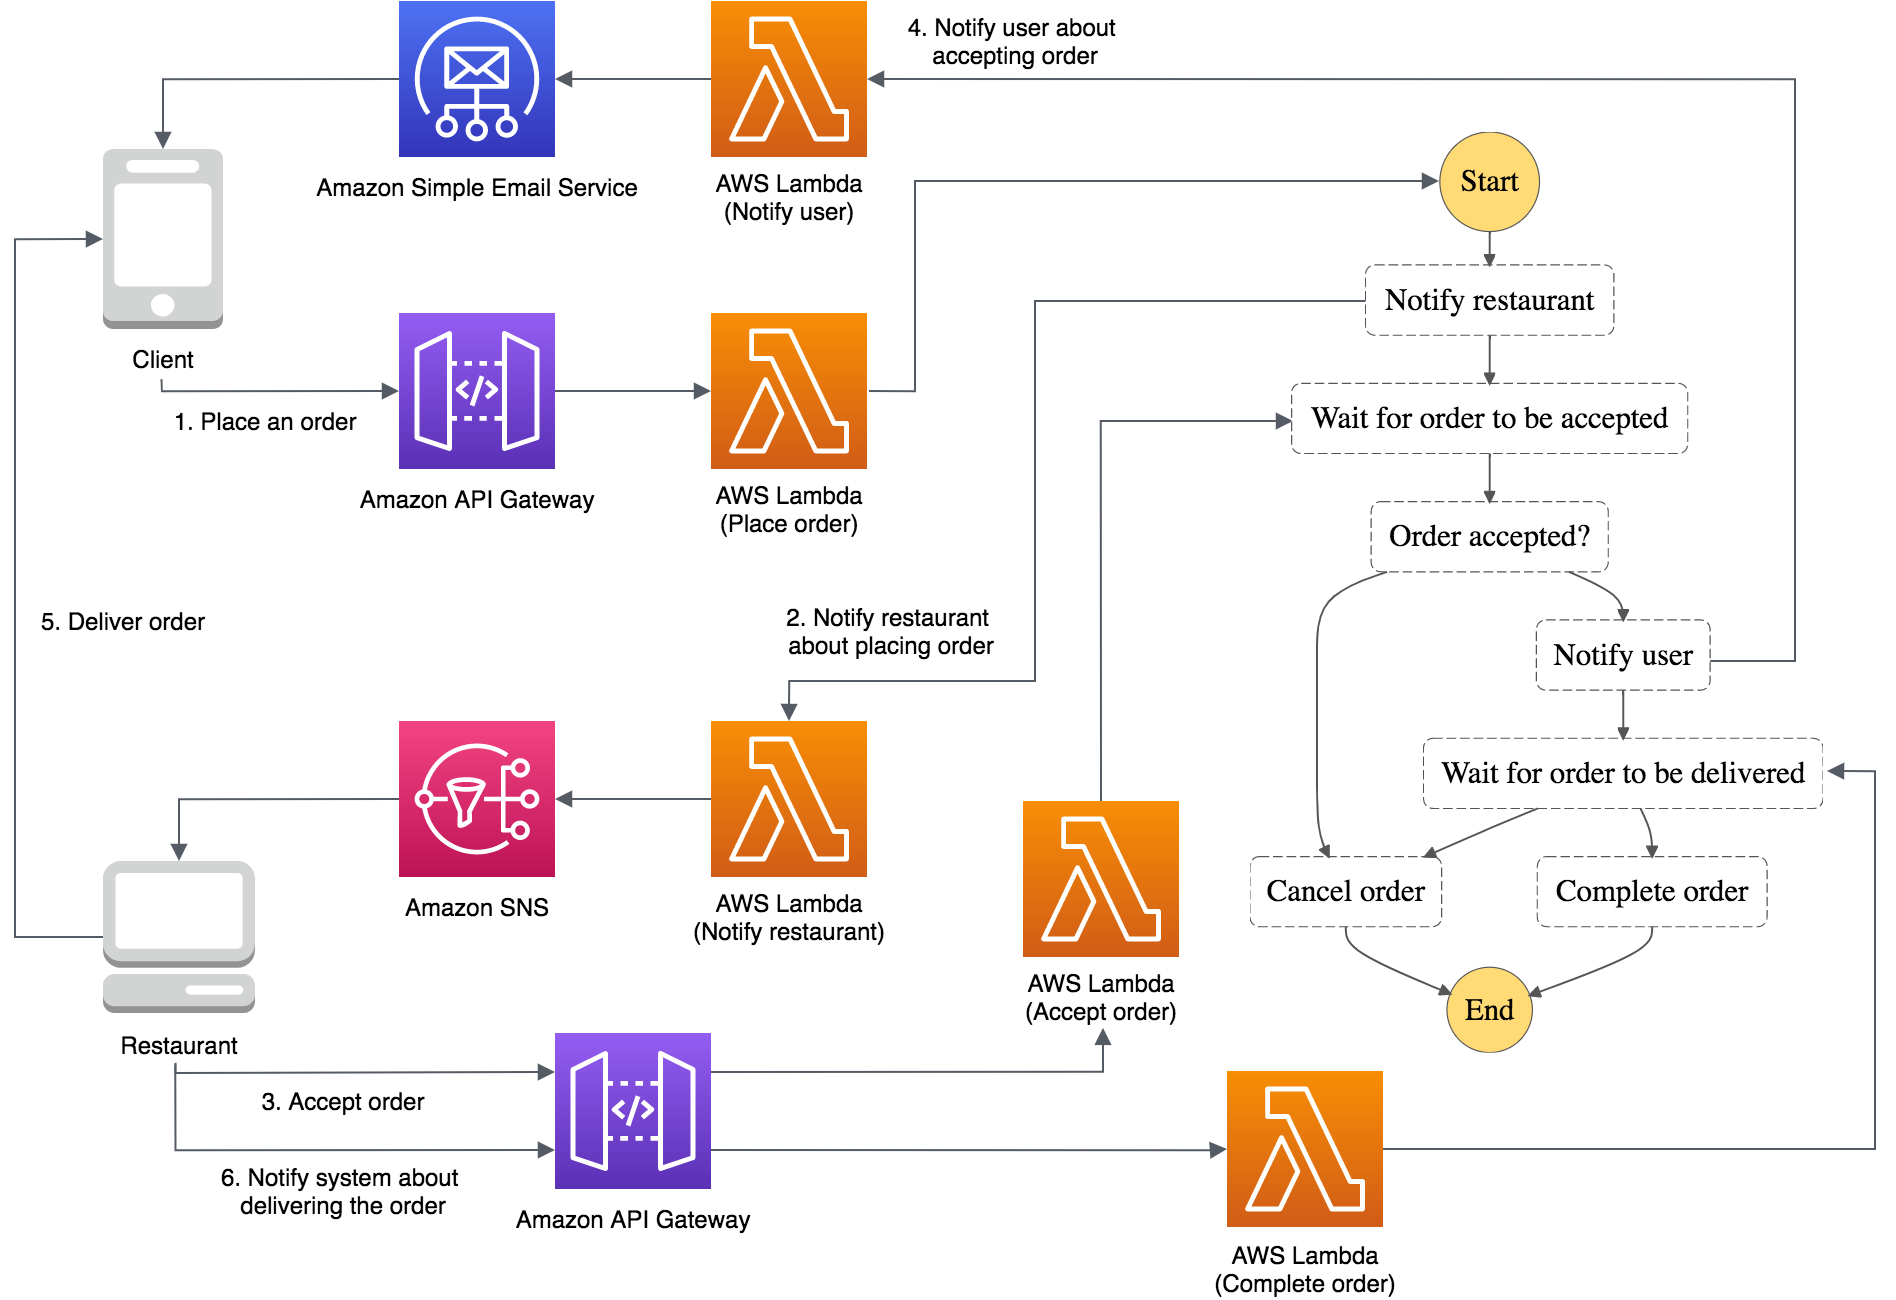
\includegraphics[width=0.8\textwidth]{assets/04-serverless-for-web-apps/orchestration.png}
   \caption{The food delivery workflow modeled using the orchestration approach}
   \label{fig:orchestration-diagram}
\end{figure}

Moreover, the orchestration approach using the Step Function is suitable for using the distributed saga pattern \cite{SagaPattern} to coordinate the distributed transactions across multiple microservices including independent datastores.
It can be applied to coordinate some more complex processes including multiple operations, which can fail during the processing and require orchestrating a series of compensating transactions, reverting the executed operations and cleaning up the state.
An example of such orchestration workflow is presented in the Figure \ref{fig:saga-orchestration-diagram}, covering the multistep booking process.

\begin{figure}[H]
   \centering
   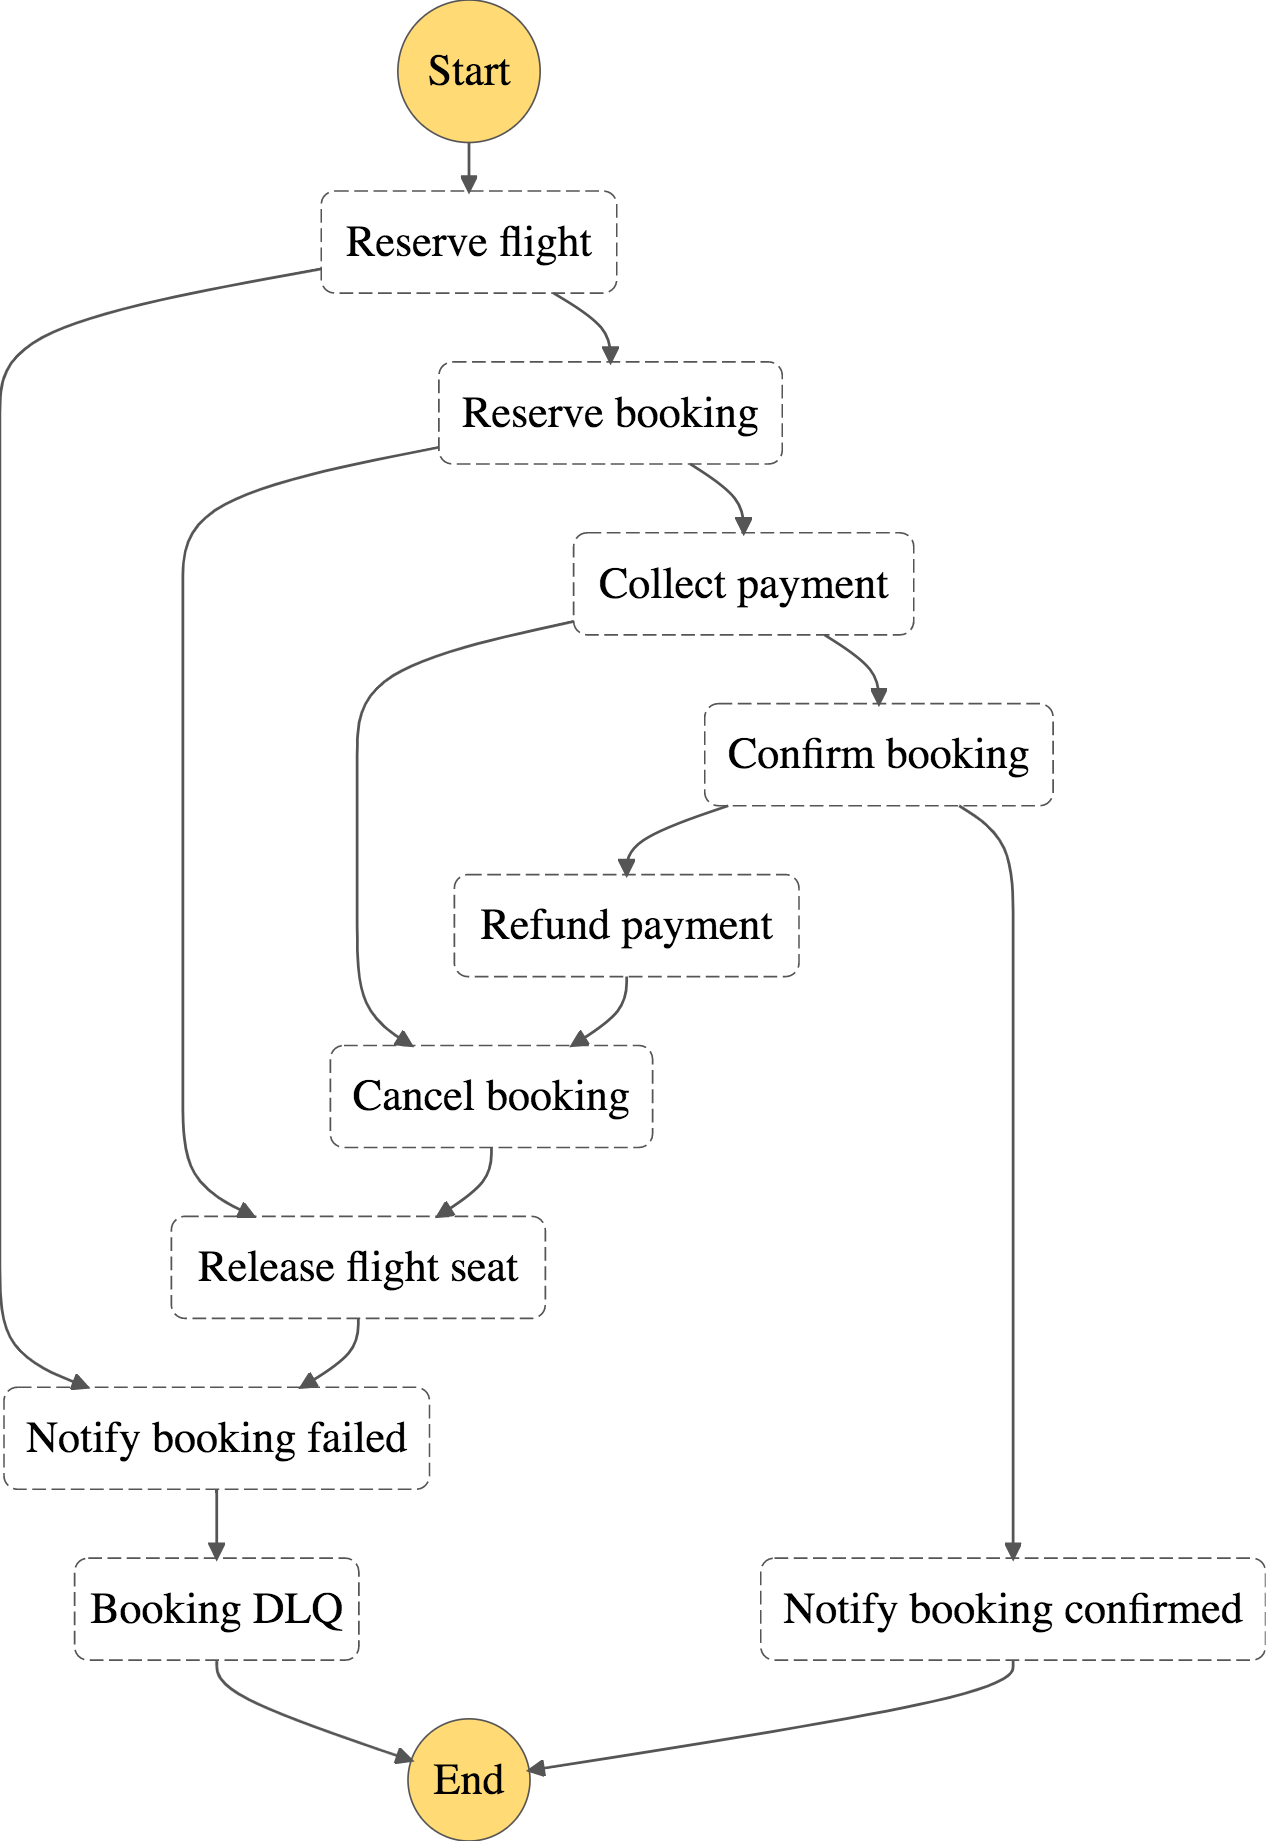
\includegraphics[width=0.5\textwidth]{assets/04-serverless-for-web-apps/saga.png}
   \caption{The multistep booking workflow using the distributed saga pattern}
   \label{fig:saga-orchestration-diagram}
\end{figure}

\subsection{Case study - Generating interactive slideshow based on LaTeX files} \label{chapter:latex-processing-optimisation}

The following section describes in more details the optimisation process behind the second example implementation of the web application using the serverless technology introduced in section \ref{chapter:examples-generating-interactive-slideshow-based-on-latex-files}.
The Step Function is used in the designed solution to coordinate the processing of several AWS Lambda instances that perform the processing of the individual stages in the entire flow.

In the presented research, the tests and measurements of the individual processing steps and their configurations are conducted based on the two example presentations prepared using the LaTeX typesetting system.
Both of the sample presentations, described in more details below, resemble the exercises which could be used in the mentioned service and characterise with different levels of complexity due to their content.

\begin{itemize}
   \item Exercise 1 --- Covers the 71 page long presentation that includes the solution derivation for the trigonometric equation.
   \item Exercise 2 --- Is more demanding and larger, 103 page long presentation. The first part incldues graphics and describes the required steps for solving a geometry problem, with additional calculations included in the second part of the exercise.
\end{itemize}

From the initial research and experiments with the possible solutions, the process of exporting presentations to the PDF format has been identified as a bottleneck in the entire processing, taking significantly longer than the other steps when performed in parallel.
The conducted performance tests consider mainly the processing duration from the client point of view, which is calculated as a time from requesting the invocation of Step Function, until the processing results are received by the client, once the slideshow generation is completed and the assets are available in the S3 bucket.
Along with measuring the processing time, several other metrics have been gathered, giving more insight into the performance of individual steps of the processing.
Measurements preserve the preconditions listed below:

\begin{itemize}
   \item Each of the tests is performed 10 times and the presented results are the average of the conducted measurements.
   \item Initially, the infrastructure has been redeployed after each execution to ensure colds starts, however thanks to the horizontal scalability of the serverless components and further observation, the same results in terms of the processing time have been obtained when the client application performed 10 requests at the same time. 
   Each of the functions executed in parallel included the information about cold start.
   Such behaviour confirms the scaling capabilities of the application based on the serverless architecture as well as resembles the situation when several users requested the presentation within short period of time, determining the worst case in terms of observable performance when the cold starts occured.
   \item The LaTeX files related to generating the presentation are removed from the temporal disc space of the function execution container once the processing is completed.
   The operation is performed to prevent a situation, when the subsequent function execution utilises the same instance of the serverless function and can benefit from the intermediate processing results from the previous invocation, which could affect the warm start execution results.
\end{itemize}

\subsubsection{Custom Lambda container image and Lambda layer}

As mentioned before, generating of the presentation based on the LaTeX file can be classified as a custom type of processing for the serverless function runtime, that goes beyond the standard set of its tasks. The section \ref{chapter:lambda-custom-runtimes} discusses in more details the possibilities of the serverless platform in terms of performing such non-standard tasks. The following section presents the results of generating the PDF file with presentation using two approaches:

\begin{itemize}
   \item Container image --- uses the official Amazon container image for Node.js runtime with additional LaTeX distribution and other libraries required for the processing.
   \item Lambda layer --- includes the LaTeX distribution extracted from the aforementioned container image into the separate archive along with the additional Lambda layer including the Perl interpreter required for the file processing.
\end{itemize}

Both of the approaches execute the same function code running in the Node.js runtime, using the provided LaTeX distribution to generate the presentation.

\pgfplotstableread{
% xaxis1, xaxis2, Layer Cold, Layer Warm, Image Cold, Image Warm
0.225 0.275 5.455 2.147 7.943 2.209
0.725 0.775 9.469 5.235 10.832 5.210
}\datasetLayerVsImage

\begin{figure}[H]
    \begin{tikzpicture}
    \begin{axis}[ybar,
        width=.9\textwidth,
        ymin=0,
        ymax=12,        
        xmin=0,
        xmax=1,        
        ylabel={Response time [s]},
        bar width=4ex,
        xtick=data,
        xticklabels = {Exercise 1, Exercise 2},
        x tick label style={align=center,xshift=2ex},
        major x tick style = {opacity=0},
        minor tick length=1ex,
        legend style={at={(0.49,0.99)},anchor=north east},
        ]
            
    \addplot[draw=black,fill=blue!40,error bars/.cd,y dir=both,y explicit] 
        table[x index=0,y index=2] \datasetLayerVsImage; % Layer Cold
    \addplot[draw=black,fill=red!40,error bars/.cd,y dir=both,y explicit] 
        table[x index=0,y index=3] \datasetLayerVsImage; % Layer Warm
    \addplot[draw=black,fill=blue!70,error bars/.cd,y dir=both,y explicit] 
        table[x index=1,y index=4] \datasetLayerVsImage; % Image Cold
    \addplot[draw=black,fill=red!70,error bars/.cd,y dir=both,y explicit] 
        table[x index=1,y index=5] \datasetLayerVsImage; % Image Warm
    \legend{Lambda layer - cold start, Lambda layer - warm start, container image - cold start, container image - warm start}
    \end{axis}
    \end{tikzpicture}
    \caption{Response time comparison of the solutions using custom container image for AWS Lambda and Lambda layers with the LaTeX distribution}
    \label{chart:step-function-lambda-layer-vs-container-image}
\end{figure}

Key takeaways of the container image and Lambda layer processing comparison:

\begin{itemize}
    \item \textbf{Cold start times} --- The significant processing time difference can be noticed when comparing the executions with cold and warm starts.
    The cold start time can be further divided into two parts. The first one considers the overhead related with the resource allocation from the large resource pool hosted by the cloud provider, downloading the function code and starting new, ephemeral container to execute the function.
    The second part is related with bootstrapping the function runtime as well as initialising dependencies required to execute the function handler.
    The detailed results of the cold start analysis are presented in the Table \ref{table:impact-of-the-cold-start-on-the-presentation-processing-task-for-approach-using-lambda-layer} and \ref{table:impact-of-the-cold-start-on-the-presentation-processing-task-for-approach-using-lambda-container-image}.

    \begin{table}[h]
        \centering
        \begin{tabular}{ |c|c|c|c|c|c| } 
        \hline
        Exercise & Execution & Function [ms] & Environment [ms] & Runtime [ms] & Execution [ms] \\
        \hline
        \multirow{2}{*}{Exercise 1} & cold start & 3609 & 914 & 273 & 2422 \\
        & warm start & 1614 & 34 & 0 & 1580 \\
        \hline
        \multirow{2}{*}{Exercise 2} & cold start & 7802 & 468 & 279 & 7055 \\
        & warm start & 4661 & 52 & 0 & 4609 \\
        \hline
        \end{tabular}
        \caption{Impact of the cold start on the presentation processing task for approach using Lambda layer}
        \label{table:impact-of-the-cold-start-on-the-presentation-processing-task-for-approach-using-lambda-layer}
    \end{table}

    \begin{table}[h]
        \centering
        \begin{tabular}{ |c|c|c|c|c|c| } 
        \hline
        Exercise & Execution & Function [ms] & Environment [ms] & Runtime [ms] & Execution [ms] \\
        \hline
        \multirow{2}{*}{Exercise 1} & cold start & 6548 & 637 & 1108 & 4803 \\
        & warm start & 1638 & 45 & 0 & 1593 \\
        \hline
        \multirow{2}{*}{Exercise 2} & cold start & 8945 & 316 & 810 & 7819 \\
        & warm start & 4614 & 35 & 0 & 4579 \\
        \hline
        \end{tabular}
        \caption{Impact of the cold start on the presentation processing task for approach using custom container image for Lambda}
        \label{table:impact-of-the-cold-start-on-the-presentation-processing-task-for-approach-using-lambda-container-image}
    \end{table}

    The runtime initialisation time of the solution using Lambda layer is comparable for both exercises and it is equal on the average to 273 ms and 279 ms for Exercise 1 and Exercise 2 accordingly. 
    For the processing using the container image solution, the runtime initialisation time is on the average equal to 1108 ms and 810 ms, which has a visible impact on the overall processing time. Moreover, the runtime initialisation time for the solution based on the container image is additionally billed accordingly to AWS Lambda pricing, on the contrary to the approach using the Lambda layer in which the cold start time is not included into the cost.
    The processing performance evaluation for the Exercise 1 preceded the Exercise 2, which could explain the decrease of the time required to download the function code and allocate resources.
    \item \textbf{Warm start times} --- When considering the prewarmed function environments, there is no visible difference in the overall processing time between both of the tested solutions.
    \item \textbf{Step Function overhead} --- The orchestration overhead computed as the overall processing time of the Step Function decreased by the time of particular tasks defined in the Step Function flow, ranges from 400 ms and 450 ms, for both cold and warm starts.    
\end{itemize}

Based on the results of the comparison the Lambda layer is selected as a more suitable solution for further workflow optimisation.

\subsubsection{Function chain length}

In the previous section, the task of generating PDF presentations from the LaTeX files is discussed, however the flow proposed in section \ref{chapter:examples-generating-interactive-slideshow-based-on-latex-files-proposed-processing-flow} describes the additional step of extracting the individual slides of the presentation to SVG files. To achieve this, the lightweight \textit{pdf2svg} \cite{pdf2svg} library is used. The following scenario measures the processing performance in two configurations:

\begin{itemize}
   \item Single function --- the conversion is performed in a single function that generates the presentation and extracts the slides, which are stored further in the S3 bucket.
   \item Function chain --- the processing is performed in the separate functions, storing the intermediate PDF file in the S3 bucket.
\end{itemize}

\pgfplotstableread{
% xaxis1, xaxis2, Single Cold, Single Warm, Chain Cold, Chain Warm
0.225 0.275 6.242 2.724 7.084 2.970
0.725 0.775 10.039 5.731 11.612 5.963
}\datasetChainVsSingle

\begin{figure}[H]
    \begin{tikzpicture}
    \begin{axis}[ybar,
        width=.9\textwidth,
        ymin=0,
        ymax=12,        
        xmin=0,
        xmax=1,        
        ylabel={Response time [s]},
        bar width=4ex,
        xtick=data,
        xticklabels = {Exercise 1, Exercise 2},
        x tick label style={align=center,xshift=2ex},
        major x tick style = {opacity=0},
        minor tick length=1ex,
        legend style={at={(0.465,0.99)},anchor=north east}
        ]

    \addplot[draw=black,fill=blue!40,error bars/.cd,y dir=both,y explicit] 
        table[x index=0,y index=2] \datasetChainVsSingle; % Single Cold
    \addplot[draw=black,fill=red!40,error bars/.cd,y dir=both,y explicit] 
        table[x index=0,y index=3] \datasetChainVsSingle; % Single Warm
    \addplot[draw=black,fill=blue!70,error bars/.cd,y dir=both,y explicit] 
        table[x index=1,y index=4] \datasetChainVsSingle; % Chain Cold
    \addplot[draw=black,fill=red!70,error bars/.cd,y dir=both,y explicit] 
        table[x index=1,y index=5] \datasetChainVsSingle; % Chain Warm
    \legend{Single function - cold start, Single function - warm start, Function chain - cold start, Function chain - warm start}
    \end{axis}
    \end{tikzpicture}
    \caption{Response time comparison of the solutions using single function and function chain to process the presentation}
    \label{chart:step-function-single-function-vs-function-chain}
\end{figure}

Key takeaways of the comparison:

\begin{itemize}
   \item \textbf{Keep the function chain short} --- When chaining several functions to perform some workflow, the overhead related to the communication and the cold start compounds. Additionally, the intermediate results need to be stored in some external component, which introduces additional work and latency that can be noticeable, especially when working with large volumes of the data.
   \item \textbf{Lambda layers constraints} --- The small size of the \textit{pdf2svg} library makes it suitable for adding it and its dependencies to the Lambda layer, that includes the LaTeX distribution already. However, it is crucial to take into account the limitations of the approach using the Lambda layers, described in more detail in section \ref{chapter:lambda-custom-runtimes}, because at some point it may be not possible to extend the function further.
\end{itemize}

\subsubsection{Parallel processing} \label{section:case-study-parallel-processing}

The serverless architecture is characterized by the capabilities of instant autoscaling to meet the demand of the processing.
Some types of the computation can be re-designed to utilise such feature of the architecture and improve the overall processing time by parallelising the workload.
Generating the presentation from the LaTeX files to the PDF format is a custom type of processing task, that under some circumstances can be parallelised to a certain degree as well.
The predefined range of slides from the presentation prepared using the Beamer package \cite{beamer}, can be selected using the \textit{\textbackslash includeonlyframes} directive.
However, the LaTeX files processing requires to repeat some initial and common part of the processing regardless of the selected subset of slides, which causes some part of the processing to be repeated for each of the presentation chunk.

The taken approach splits the LaTeX processing into several serverless function executions running in parallel. Each of the functions is assigned to generate the slides for predefined presentation chunks, containing 5 consecutive slides. Once the processing of all serverless functions is completed, along with the commentary transcription and metadata extraction, the user is notified about the results of the processing. The Step Function processing graph is presented in Figure \ref{fig:step-function-processing-the-presentation-in-parallel}, indicating that the presentation generation is divided into chunks, that are mapped to independent function calls and executed in parallel.

\begin{figure}[H]
    \centering
    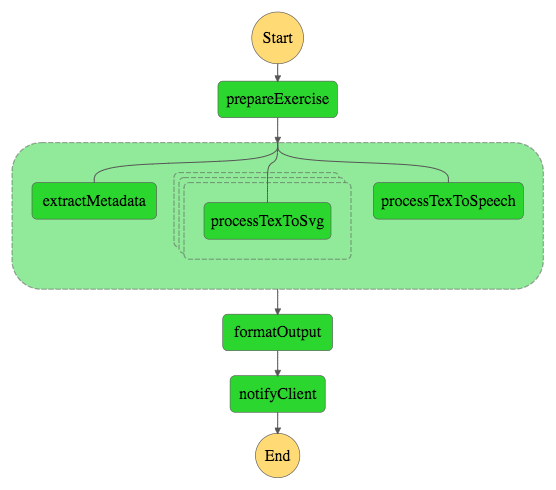
\includegraphics[width=0.6\textwidth]{assets/04-serverless-for-web-apps/stepFunctionGraphParallel.png}
    \caption{Step Function processing graph --- Generating the presentation chunks in parallel}
    \label{fig:step-function-processing-the-presentation-in-parallel}
\end{figure}

\pgfplotstableread{
% xaxis1, xaxis2, Single Cold, Single Warm, Parallel Cold, Parallel Warm
0.225 0.275 6.242 2.724 4.996 2.136
0.725 0.775 10.039 5.731 7.477 3.186
}\datasetSingleVsParallel

\begin{figure}[H]
    \begin{tikzpicture}
    \begin{axis}[ybar,
        width=.9\textwidth,
        ymin=0,
        ymax=12,        
        xmin=0,
        xmax=1,        
        ylabel={Response time [s]},
        bar width=4ex,
        xtick=data,
        xticklabels = {Exercise 1, Exercise 2},
        x tick label style={align=center,xshift=2ex},
        major x tick style = {opacity=0},
        minor tick length=1ex,
        legend style={at={(0.5175,0.99)},anchor=north east}
        ]

    \addplot[draw=black,fill=blue!40,error bars/.cd,y dir=both,y explicit] 
        table[x index=0,y index=2] \datasetSingleVsParallel; % Single Cold
    \addplot[draw=black,fill=red!40,error bars/.cd,y dir=both,y explicit] 
        table[x index=0,y index=3] \datasetSingleVsParallel; % Single Warm
    \addplot[draw=black,fill=blue!70,error bars/.cd,y dir=both,y explicit] 
        table[x index=1,y index=4] \datasetSingleVsParallel; % Parallel Cold
    \addplot[draw=black,fill=red!70,error bars/.cd,y dir=both,y explicit] 
        table[x index=1,y index=5] \datasetSingleVsParallel; % Parallel Warm
    \legend{Single function - cold start, Single function - warm start, Parallel processing - cold start, Parallel processing - warm start}
    \end{axis}
    \end{tikzpicture}
    \caption{Response time comparison of the solutions using single function to generate the complete presentation and the parallelised processing of separate chunks}
    \label{chart:step-function-single-function-vs-parallel-processing}
\end{figure}

Key takeaways of the parallel processing compared to the single function execution:

\begin{itemize}
    \item \textbf{Parallelising the LaTeX files processing} --- Even though the presentation generation processing cannot be effectively parallelised, the overall processing time is reduced for both of the provided examples.
    The complexity of the selected examples has a significant impact on the total processing time.
    When measuring and comparing the processing time on the local machine, generating the chunks independently for the Exercise 1 reduced the overall processing time by 32\%, while for the Exercise 2 it reached approximately 74\%, that confirms the previous statement.
  
    The average execution time for the presentation generation task of the chunks processed in separate functions compared to processing of the complete presentation in a single function is presented in Table \ref{table:overhead-of-the-presentation-processing-task-for-the-whole-presentation-and-chunks-including-5-slides}

    \begin{table}[h]
        \centering
        \begin{tabular}{ |c|c|c|c|c|c| } 
        \hline
        Exercise & Execution & Complete [ms] & Avg. of chunks [ms] & Time reduction [\%] \\
        \hline
        \multirow{2}{*}{Exercise 1} & cold start & 3349 & 2748 & 17.95 \\
        & warm start & 1641 & 1100 & 32.97 \\
        \hline
        \multirow{2}{*}{Exercise 2} & cold start & 7887 & 4310 & 45.35 \\
        & warm start & 4679 & 1313 & 71.94 \\
        \hline
        \end{tabular}
        \caption{Time reduction of the presentation processing task for the complete presentation and chunks including 5 slides}
        \label{table:overhead-of-the-presentation-processing-task-for-the-whole-presentation-and-chunks-including-5-slides}
    \end{table}

   \item \textbf{Orchestrating parallel processing brings additional overhead} --- It is essential to consider the additional overhead related to the orchestration of several serverless functions processing the presentation chunks in parallel. In the following example, the orchestration overhead is calculated as the Step Function duration decreased by the average tasks duration. It is equal to 873 ms (cold start) and 890 ms (warm start) for Exercise 1 as well as 1765 ms (cold start) and 1745 ms (warm start) for Exercise 2.
   \item \textbf{Cost of the parallel processing} --- Besides the processing overhead, the parallel execution brings additional cost for each of the executed serverless functions and its execution time. Moreover, for the given example the processing cannot be effectively parallelised and some part of the processing and retrieving the file is repeated for each invoked function, impacting the overall cost of the computation.
\end{itemize}

\subsubsection{Updating the client with processed batches} \label{section:case-study-updating-the-client-with-processed-batch}

The approach presented in the previous section enables to effectively parallelise the processing and reduce the overall processing time, but it is restricted by the fact that all of the presentation chunks needs to be processed to push the update to the client. When taking into consideration how the presentations are prepared, most frequently the first several slides include the introduction to the exercise that usually takes more than 10 seconds. From the user perspective, only the first batch is required to start presenting the slideshow, while the remaining part of the assets can be delivered later.

The further improvements of the processing flow takes into account the aforementioned assumption and parallelises the presentation processing on the higher level, to deliver the updates of the processed presentation chunks independently. The Step Function processing graph of suggested approach is presented in Figure \ref{fig:step-function-pushing-updates-to-the-client-with-partially-processed-presentation}. The further measurements reflects the response time for two configurations of the flow, described below:

\begin{itemize}
   \item First batch with 5 initial slides processed and the second batch with the remaining part of the presentation --- the processing is effectively parallelised in two branches.
   \item Each of the batches include information about 5 consecutive slides --- the processing is parallelised depending on the size of the presentation, with each of the branches processing 5 consecutive slides.
\end{itemize}

The results of the processing are compared with processing time of the complete presentation by a single serverless function and when the processing is parallelised, as shown in the previous section. The results are presented in the figures \ref{chart:step-function-initial-batch} and \ref{chart:step-function-batches}.

\begin{figure}[H]
    \centering
    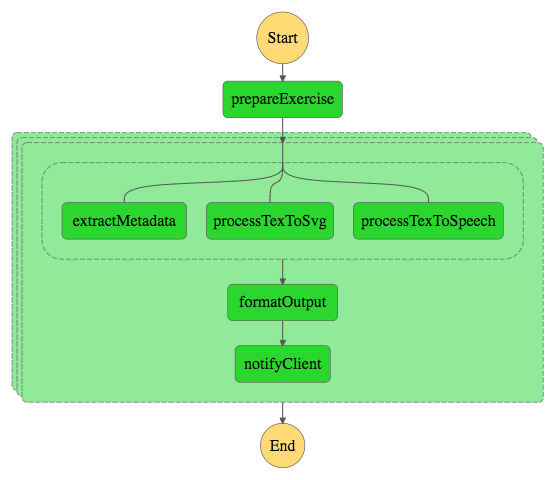
\includegraphics[width=0.6\textwidth]{assets/04-serverless-for-web-apps/stepFunctionGraphInitialBatch.png}
    \caption{Step Function processing graph --- Delivering updates to the client with independently processed presentation chunks}
    \label{fig:step-function-pushing-updates-to-the-client-with-partially-processed-presentation}
\end{figure}

\pgfplotstableread{
% xaxis, Single Cold, Single Warm, Parallel Cold, Parallel Warm, FirstBatch Cold, RestBatch Cold, FirstBatch Warm, RestBatch Warm
0.25 6.242 2.724 4.996 2.136 4.315 4.680 1.710 2.718
0.75 10.039 5.731 7.477 3.186 5.611 9.755 1.803 5.814
}\datasetUploadInitialBatch

\begin{figure}[H]
    \begin{tikzpicture}
    \begin{axis}[ybar,
        width=.9\textwidth,
        ymin=0,
        ymax=12,        
        xmin=0,
        xmax=1,
        bar width=3ex,  
        ylabel={Response time [s]},
        xtick=data,
        xticklabels = {Exercise 1,Exercise 2},
        major x tick style = {opacity=0},
        minor x tick num = 1,
        minor tick length=1ex,
        legend style={at={(0.5,0.99)},anchor=north east}
        ]
    \addplot[draw=black,fill=blue!40,error bars/.cd,y dir=both,y explicit] 
        table[x index=0,y index=1] \datasetUploadInitialBatch; % Single Cold
    \addplot[draw=black,fill=red!40,error bars/.cd,y dir=both,y explicit] 
        table[x index=0,y index=2] \datasetUploadInitialBatch; % Single Warm
    \addplot[draw=black,fill=blue!70,error bars/.cd,y dir=both,y explicit] 
        table[x index=0,y index=3] \datasetUploadInitialBatch; % Parallel Cold
    \addplot[draw=black,fill=red!70,error bars/.cd,y dir=both,y explicit] 
        table[x index=0,y index=4] \datasetUploadInitialBatch; % Parallel Warm
    \addplot[draw=black,fill=blueDark!50,error bars/.cd,y dir=both,y explicit] 
        table[x index=0,y index=5] \datasetUploadInitialBatch; % FirstBatch Cold
    \addplot[draw=black,fill=blueDark!80,error bars/.cd,y dir=both,y explicit] 
        table[x index=0,y index=6] \datasetUploadInitialBatch; % RestBatch Cold
    \addplot[draw=black,fill=redDark!50,error bars/.cd,y dir=both,y explicit] 
        table[x index=0,y index=7] \datasetUploadInitialBatch; % FirstBatch Warm
    \addplot[draw=black,fill=redDark!80,error bars/.cd,y dir=both,y explicit] 
        table[x index=0,y index=8] \datasetUploadInitialBatch; % RestBatch Warm
    \legend{Single function - cold start, Single function - warm start, Parallel execution - cold start, Parallel execution - warm start, First batch - cold start, Second batch - cold start, First batch - warm start, Second batch - warm start}
    \end{axis}
    \end{tikzpicture}
    \caption{Response time comparison of the solution delivering the update to the client in the first batch including initial 5 slides and the second batch with remaining data}
    \label{chart:step-function-initial-batch}
\end{figure}

\pgfplotstableread{
% xaxis, Single Cold, Single Warm, Parallel Cold, Parallel Warm, FirstBatch Cold, RestBatch Cold, FirstBatch Warm, RestBatch Warm
0.25 6.242 2.724 4.996 2.136 12.615 12.867 11.792 12.366
0.75 10.039 5.731 7.477 3.186 22.563 22.948 22.209 22.374
}\datasetUploadBatches

\begin{figure}[H]
    \begin{tikzpicture}
    \begin{axis}[ybar,
        width=.9\textwidth,
        ymin=0,
        ymax=24,        
        xmin=0,
        xmax=1,
        bar width=3ex,  
        ylabel={Response time [s]},
        xtick=data,
        xticklabels = {Exercise 1,Exercise 2},
        major x tick style = {opacity=0},
        minor x tick num = 1,
        minor tick length=1ex,
        legend style={at={(0.5,0.99)},anchor=north east}
        ]
    \addplot[draw=black,fill=blue!40,error bars/.cd,y dir=both,y explicit] 
        table[x index=0,y index=1] \datasetUploadBatches; % Single Cold
    \addplot[draw=black,fill=red!40,error bars/.cd,y dir=both,y explicit] 
        table[x index=0,y index=2] \datasetUploadBatches; % Single Warm
    \addplot[draw=black,fill=blue!70,error bars/.cd,y dir=both,y explicit] 
        table[x index=0,y index=3] \datasetUploadBatches; % Parallel Cold
    \addplot[draw=black,fill=red!70,error bars/.cd,y dir=both,y explicit] 
        table[x index=0,y index=4] \datasetUploadBatches; % Parallel Warm
    \addplot[draw=black,fill=blueDark!50,error bars/.cd,y dir=both,y explicit] 
        table[x index=0,y index=5] \datasetUploadBatches; % FirstBatch Cold
    \addplot[draw=black,fill=blueDark!80,error bars/.cd,y dir=both,y explicit] 
        table[x index=0,y index=6] \datasetUploadBatches; % RestBatch Cold
    \addplot[draw=black,fill=redDark!50,error bars/.cd,y dir=both,y explicit] 
        table[x index=0,y index=7] \datasetUploadBatches; % FirstBatch Warm
    \addplot[draw=black,fill=redDark!80,error bars/.cd,y dir=both,y explicit] 
        table[x index=0,y index=8] \datasetUploadBatches; % RestBatch Warm
    \legend{Single function - cold start, Single function - warm start, Parallel execution - cold start, Parallel execution - warm start, First batch - cold start, All batches - cold start, First batch - warm start, All batches - warm start}
    \end{axis}
    \end{tikzpicture}
    \caption{Response time comparison of the solution delivering the update to the client in the separate batches}
    \label{chart:step-function-batches}
\end{figure}

Key takeaways of the proposed approach:

\begin{itemize}
   \item \textbf{Improved response time of the initial batch} --- For the first of the considered configurations, with the results presented in Figure \ref{chart:step-function-initial-batch}, the response time for the first batch including the first slides is shorter.
   Once it is received by the client, the user can start previewing the slideshow, while the second batch including the remaining data can be processed and received by the client later.
   Such a solution enables the user to start previewing the exercise quicker, while the processing time of the complete presentation is hidden from the user perspective.
   \item \textbf{Increase of the Step Function overhead for the fine-grained workflow coordination} --- In the second configuration that splits the presentation chunks equally and parallelises the processing, the overhead of the Step Function responsible for the orchestration makes the processing significantly longer.
   Moreover, the batch including 5 initial slides is frequently delivered as one of the latests, significantly postponing the time when the user can start previewing the exercise, as it is presented in the Figure \ref{chart:step-function-batches}.
\end{itemize}

\subsubsection{Comparing serverless solution with the traditional architecture}

When deciding on the serverless architecture, there is always a question how the solution will perform compared to the solution implemented using the more traditional architectures.
To answer that question for the given problem, a similar service based on a simple server running within the container has been created and hosted on the AWS Fargate. 
The server is executed in the Node.js runtime, similarly to the serverless functions from the previous steps of the study.
Moreover, it is reusing a significant part of the logic responsible for the initial validation of the task, processing the LaTeX presentation to PDF and then extracting separate slides to the SVG files, using the same libraries as well as uploading the results to S3 once the processing is completed.
The container is configured with the same amount of memory and CPU as the serverless function used for the processing in the serverless implementation.

The figure \ref{chart:step-function-compared-with-traditional-architecture} presents how the solution using the traditional architecture performs compared with the various configurations of the serverless solution.

\pgfplotstableread{
% xaxis, Single Cold, Single Warm, Parallel Cold, Parallel Warm, FirstBatch Cold, RestBatch Cold, FirstBatch Warm, RestBatch Warm
0.25 6.242 2.724 4.996 2.136 4.315 4.680 1.710 2.718 2.636
0.75 10.039 5.731 7.477 3.186 5.611 9.755 1.803 5.814 6
}\datasetCompareContainer

\begin{figure}[H]
    \begin{tikzpicture}
    \begin{axis}[ybar,
        width=.9\textwidth,
        ymin=0,
        ymax=12,        
        xmin=0,
        xmax=1,
        bar width=3ex,  
        ylabel={Response time [s]},
        xtick=data,
        xticklabels = {Exercise 1,Exercise 2},
        major x tick style = {opacity=0},
        minor x tick num = 1,
        minor tick length=1ex,
        legend style={at={(0.5,0.99)},anchor=north east}
        ]
    \addplot[draw=black,fill=blue!40,error bars/.cd,y dir=both,y explicit] 
        table[x index=0,y index=1] \datasetCompareContainer; % Single Cold
    \addplot[draw=black,fill=red!40,error bars/.cd,y dir=both,y explicit] 
        table[x index=0,y index=2] \datasetCompareContainer; % Single Warm
    \addplot[draw=black,fill=blue!70,error bars/.cd,y dir=both,y explicit] 
        table[x index=0,y index=3] \datasetCompareContainer; % Parallel Cold
    \addplot[draw=black,fill=red!70,error bars/.cd,y dir=both,y explicit] 
        table[x index=0,y index=4] \datasetCompareContainer; % Parallel Warm
    \addplot[draw=black,fill=blueDark!50,error bars/.cd,y dir=both,y explicit] 
        table[x index=0,y index=5] \datasetCompareContainer; % FirstBatch Cold
    \addplot[draw=black,fill=blueDark!80,error bars/.cd,y dir=both,y explicit] 
        table[x index=0,y index=6] \datasetCompareContainer; % RestBatch Cold
    \addplot[draw=black,fill=redDark!50,error bars/.cd,y dir=both,y explicit] 
        table[x index=0,y index=7] \datasetCompareContainer; % FirstBatch Warm
    \addplot[draw=black,fill=redDark!80,error bars/.cd,y dir=both,y explicit] 
        table[x index=0,y index=8] \datasetCompareContainer; % RestBatch Warm
    \addplot[draw=black,fill=green!60,error bars/.cd,y dir=both,y explicit] 
        table[x index=0,y index=9] \datasetCompareContainer; % RestBatch Warm
    \legend{Single function - cold start, Single function - warm start, Parallel execution - cold start, Parallel execution - warm start, First batch - cold start, Second batch - cold start, First batch - warm start, Second batch - warm start, Container environment}
    \end{axis}
    \end{tikzpicture}
    \caption{Response time comparison of the solutions using the serverless and traditional architectures}
    \label{chart:step-function-compared-with-traditional-architecture}
\end{figure}

Key takeaways of the serverless implementation comparison with the solution using the simple, containerized server application:

\begin{itemize}
    \item \textbf{The performance of serverless implementation is comparable, when it is not affected by the cold starts} --- The initial serverless solution, orchestrating the flow and using single function to process the LaTeX file, performs similarly when executed with the warm start, compared to the solution using the simple server hosted by AWS Fargate in the container. However, when the execution is affected by the cold starts, the response time is significantly longer as presented in Figure \ref{chart:step-function-compared-with-traditional-architecture}.
    It is beneficial to consider the interest in the service as well as the traffic pattern to estimate how often such a phenomenon may take place, when deciding on architecture selection or mitigating the negative influence by pre-warming the containers programmatically or by the services, such as Provisioned Concurrency for AWS Lambda.
    \item \textbf{Re-designing the serverless processing to utilise its benefits can improve performance} --- The presented configurations of the serverless solution confirms that remodeling the processing to use the benefits of the serverless paradigm can bring visible benefits in terms of the performance, compared to the solution using the more traditional architecture.
    However, some aspects and tasks of the proposed flow are required for the serverless solution, such as uploading the results of processing to S3, which could be further accessed by the user.
    The solution using the server could aggregate the results of processing locally, without the need to communicate with external component to store the files and return the results directly to the user, reducing the amount of work and cost.
    \item \textbf{Built-in scalability of the serverless architecture} --- One of the features of the serverless architecture is the possibility of almost instant and effortless processing parallelisation, that reduces the overall processing time in that case.
    As mentioned in the introduction to the section, the performance tests of the executions characterised by the cold starts have been measured by sending 10 requests simultaneously, resulting with similar performance as the single executions interleaved with redeploying the infrastructure. 
    This approach allows to infer about the behaviour of the service, when several users will use the service simultaneously, while showing the worst case in terms of the service performance.
    Further research could investigate in more details, how the implementations using both of the architectures are performing under the load, resembling the behaviour of the potential users of the system.
    When considering the serverless solution, the impact could be visible by increased number of cold starts, when the traffic pattern is changing or it is occasional. However, the solution using the simple server hosted in the container could note the performance decline similarly, when many subsequent requests would be submitted to a single worker instance or when the cluster of workers would need to scale to meet the demand.
\end{itemize}

\subsubsection{Cost of the designed solution}

Another, frequently mentioned factor when deciding on the architecture choice is the maintenance and execution cost. The serverless architecture makes it more difficult to precisely measure the cost of the processing, due to the number of components and the variety of granularity in pricing model for used services. However, the cost can be quite accurately estimated, when the traffic pattern is known along with the execution cost of particular workflow.

The section calculates the cost of a single execution of the entire processing flow for Exercise 1, considering two configurations described previously:

\begin{itemize}
   \item The parallel presentation processing describes in section \ref{section:case-study-parallel-processing}.
   \item The first configuration described in section \ref{section:case-study-updating-the-client-with-processed-batch}, in which the presentation processing is divided into two branches --- first with initial slides and the second with remaining data for the slideshow completeness.
\end{itemize}

The cost of services used in the implementation is summarised in Table \ref{table:case-study-service-spendings-summary}, based on the pricing defined for region Europe (Frankfurt) and excluding the Free Tier provided by the AWS.
Cost of some of the services, such as Amazon CloudWatch for storing logs, API Gateway for the incoming traffic in form of the user requests or data transfer for DynamoDB is omitted due to negligible use and very small granularity to notice the difference in teh values of cost statement.

\begin{table}[H]
    \centering
    \begin{tabular}{ |c|c|c| } 
    \hline
    Service & Billed service usage & Pricing \\
    \hline
    \multirow{3}{*}{API Gateway} & REST API - API Calls & \$3.70 (per million) \\ 
    & WebSocket API - Connection Minutes & \$0.285 per million connection minutes \\ 
    & WebSocket API - Message Transfers & \$1.14 (per million) \\ 
    \hline
    Data Transfer & From Amazon S3 To Internet & \$0.09 per GB \\
    \hline
    \multirow{2}{*}{DynamoDB} & Read request & \$0.305 per million read request units \\
    & Write request & \$1.525 per million write request units \\
    \hline
    \multirow{2}{*}{AWS Lambda} & Duration & \$0.0000166667 for every GB-second \\
    & Requests & \$0.20 per 1M requests \\
    \hline
    Polly & Standard voices & \$4.00 per 1 million characters \\
    \hline
    \multirow{2}{*}{Simple Storage Service} & PUT, COPY, POST, LIST requests & \$0.0054 (per 1,000 requests) \\
    & GET, SELECT, and all other request & \$0.00043 (per 1,000 requests) \\
    \hline
    Step Function & State transtition & \$0.025 per 1,000 state transitions\\
    \hline
    \end{tabular}
    \caption{Pricing summary for services used in the implementations}
    \label{table:case-study-service-spendings-summary}
\end{table}

The usage of the services for both implementations and their cost is summarised in Table \ref{table:case-study-service-parallel-spending-summary} and \ref{table:case-study-service-initial-batch-spending-summary}.

\begin{table}[H]
    \centering
    \begin{tabular}{ |c|c|c| } 
    \hline
    Service usage & Usage & Cost [\$] \\
    \hline
    REST API - API Calls & 2 requests & 0,0000074 \\
    WebSocket API - Connection Minutes & 2 minutes & 0,00000057 \\
    WebSocket API - Message Transfers & 4 messages & 0,00000456 \\
    \hline
    Data Transfer From Amazon S3 To Internet & 0.003 GB & 0,00027 \\
    \hline
    DynamoDB Read request & 1 Read Request Unit & 0,0000000305 \\
    DynamoDB Write request & 2 Write Request Unit & 0,0000000305 \\
    \hline
    AWS Lambda - Duration & 61.057 GB-second & 0,00102 \\
    AWS Lambda - Requests & 22 requests & 0,0000044 \\
    \hline
    Amazon Polly - Standard voices & 1323 characters & 0,00529 \\
    \hline
    S3 PUT, COPY, POST, LIST requests & 86 requests & 0,000464 \\
    S3 GET, SELECT, and all other request & 108 requests & 0,0000464 \\
    \hline
    Step Function - state transitions & 24 transitions & 0,0006 \\
    \hline
    \multicolumn{1}{c|}{} & \textbf{Total} & 0,00771 \\
    \cline{2-3}
    \end{tabular}
    \caption{Cost summary for the approach using parallel presentation processing}
    \label{table:case-study-service-parallel-spending-summary}
\end{table}

\begin{table}[H]
    \centering
    \begin{tabular}{ |c|c|c| } 
    \hline
    Service usage & Usage & Cost [\$] \\
    \hline
    REST API - API Calls & 2 requests & 0,0000074 \\
    WebSocket API - Connection Minutes & 4 minutes & 0,00000114 \\
    WebSocket API - Message Transfers & 5 messages & 0,0000057 \\
    \hline
    Data Transfer From Amazon S3 To Internet & 0.003 GB & 0,00027 \\
    \hline
    DynamoDB Read request & 1,5 Read Request Unit & 0,0000000456 \\
    DynamoDB Write request & 2 Write Request Unit & 0,0000000305 \\
    \hline
    AWS Lambda - Duration & 11.649 GB-second & 0,000194 \\
    AWS Lambda - Requests & 12 requests & 0,0000024 \\
    \hline
    Amazon Polly - Standard voices & 1323 characters & 0,00529 \\
    \hline
    S3 PUT, COPY, POST, LIST requests & 86 requests & 0,000464 \\
    S3 GET, SELECT, and all other request & 98 requests & 0,0000421 \\
    \hline
    Step Function - state transitions & 17 transitions & 0,000425 \\
    \hline
    \multicolumn{1}{c|}{} & \textbf{Total} & 0,00671 \\
    \cline{2-3}
    \end{tabular}
    \caption{Cost summary for the approach delivering the updates to the client in separate batches}
    \label{table:case-study-service-initial-batch-spending-summary}
\end{table}

Takeaways of the cost summary of designed solutions:

\begin{itemize}
   \item \textbf{AWS Lambda processing is a small fraction of overall cost} --- Cost summaries for both of the presented solutions indicate that the text-to-voice transcoding service takes a significant amount of the overall cost.
   The usage of the AWS Lambda processing is greater for the solution using parallel processing.
   Even though some part of the presentation processing is repeated in the serverless functions executed in parallel, the overall cost of the AWS Lambda related services barely exceeds 0.001\$ for the analysed example per single workflow execution.
   Moreover, it is crucial to consider the cost of other services incorporated in the processing as well as the data transfer.
   For example, the summary of the second configuration indicates that the cost of uploading results to Amazon S3 and transferring them to the client exceeded the cost of the processing of the AWS Lambda.
   \item \textbf{Serverless pay-per-use billing model} --- Considering the Exercise 2, which is a more demanding task in terms of the processing and the summaries listed above, the overall cost of the processing for a single presentation could be estimated as not exceeding 0.01\$ per execution.
   Moreover, when taking into account the benefits of the serverless architecture, such as autoscaling with granular billing model based on usage and without paying for idle as well as the fact that the infrastructure management is handled by the cloud provider, the serverless solution with pay-per-use pricing can be an appealing alternative to more traditional architectures.
\end{itemize}

\section{Data Tier} \label{chapter:serverless-datastores}

\subsection{Issues when integrating traditional databases with serverless}

\subsection{Serverless databases}


% https://youtu.be/hwnNbLXN4vA
% https://thenewstack.io/what-front-end-developers-need-to-know-about-serverless-databases/
% https://www.alexdebrie.com/posts/dynamodb-no-bad-queries/
% https://www.alexdebrie.com/posts/dynamodb-patterns-serverless/
% https://www.trek10.com/blog/dynamodb-single-table-relational-modeling/?sc_channel=sm&sc_campaign=DB_Blog&sc_publisher=TWITTER&sc_country=DynamoDB&sc_geo=GLOBAL&sc_outcome=awareness&trk=ddbfromrelationaldbto_082720_TWITTER&sc_category=Amazon+DynamoDB&linkId=97421072

% Leadership session: AWS purpose-built databases - https://youtu.be/q81TVuV5u28
% Data modeling with Amazon DynamoDB - https://youtu.be/DIQVJqiSUkE
% Amazon DynamoDB Under the Hood: How We Built a Hyper-Scale Database - https://youtu.be/yvBR71D0nAQ
% Databases on AWS: The Right Tool for the Right Job - https://youtu.be/-pb-DkD6cWg

DynamoDB - modeling for cost optimisation, increase performance, single table design

Aurora

S3

how they work? streams, handling reusing connections, RDS proxy

---

RDS Proxy

% \cite{ServerlessAtScaleDesignPatternsAndOptimizations}
- pool and share database connection of the RDS databases
- lambda connects to proxy and proxy connects to database
- preserves connections during DB failover
- Proxy manages credentials with Secret Manager and IAM - proxy can manage credentials, lambda can have access only to the proxy

\section{Client Tier}

\subsection{Client communication patterns for serverless architecture} \label{chapter:serverless-client-communication-patterns-for-serverless-architecture}

% https://youtu.be/yfJZc3sJZ8E - Gateway
% https://serialized.net/2020/09/multiplayer/ - WebSocket applicability
% https://youtu.be/XVU4pYeNfNo - AppSync
% https://hackernoon.com/using-protocol-buffers-with-api-gateway-and-aws-lambda-22c3804f3e76 - Protobufs
% https://www.alexdebrie.com/posts/api-gateway-elements/#!newthread

APIGateway - REST + websockets

AppSync - GraphQL - data aggregation from different resources

gatekeeper - authentication

direct resolvers to particular services with/without the lambda, pipeline resolvers (nested nodes in graph) - overhead comparison

calling the services from the client - presigned URLs / using client libs to have access to resources

\subsection{Serverless push based approach}

- API Gateway authorizers
% - Power modern serverless applications with GraphQL and AWS AppSync - https://youtu.be/IcrrsbYhZoQ
% - API patterns and architectures: RESTful vs. GraphQL APIs - https://youtu.be/pBFStsa0h-4

% https://youtu.be/08AjVGGQaKQ?t=817
- Lambda authorizers

% https://aws.amazon.com/blogs/compute/from-poll-to-push-transform-apis-using-amazon-api-gateway-rest-apis-and-websockets/

% Backend-less URL shortener
% https://aws.amazon.com/blogs/compute/building-a-serverless-url-shortener-app-without-lambda-part-1/

However, for the particular services, the communication can be simplified and the API Gateway can communicate directly with various services, alleviating the need to use Lambda.

% \cite{ServerlessAtScaleDesignPatternsAndOptimizations}
% https://youtu.be/dzU_WjobaRA?t=2391

% cherry pick - GraphQL API
% https://youtu.be/9IYpGTS7Jy0?t=961

request - response

poll to push pattern

GraphQL subscriptions triggered by mutation

\subsection{Hosting web clients}

hosting static files

server side rendering

\subsection{Thick and thin client}

% how serverless affects thicker/thinner client
% direct access to service
